%\pdfoutput=1

%\documentclass[twocolumn,aps,prl,showpacs,superscriptaddress]{revtex4-1}
%\documentclass[twocolumn,aps,pra,showpacs,superscriptaddress]{revtex4}
\documentclass[%
 %reprint,
  twocolumn,
 %superscriptaddress,
 %groupedaddress,
 %unsortedaddress,
 %runinaddress,
 %frontmatterverbose,
 % preprint,
 showpacs,
 showkeys,
 preprintnumbers,
 %nofootinbib,
 %nobibnotes,
 %bibnotes,
 amsmath,amssymb,
 aps,
 % prl,
  pra,
 % prb,
 % rmp,
 %prstab,
 %prstper,
  longbibliography,
 floatfix,
 %lengthcheck,%
 ]{revtex4-1}

\newcommand{\karl}[1]{\textcolor{blue}{#1}}
\newcommand{\karllate}[1]{\textcolor{green}{#1}}
\newcommand{\jr}[1]{\textcolor{purple}{#1}}
\newcommand{\meil}[1]{\textcolor{olive}{#1}}
\usepackage[normalem]{ulem}
\usepackage{tikz}


\usepackage{graphicx}
%\usepackage{amsmath,amssymb}
\usepackage[colorlinks=true,citecolor=blue,urlcolor=blue]{hyperref}

%\def\endproof{\vrule height6pt width6pt depth0pt}
\def\endproof{ }

%%%%%%%%%%%%%%%%%%%%%%%%%%%%%%%%%%%%%%%%%%%%%%%%%%%%%%%%%%%%%%%%%%%

\begin{document}

%josera@us.es,svozil@tuwien.ac.at,solisencina@us.es,adan@us.es

%%%%%%%%%%%%%%%%%%%%%%%%%%%%%%%%%%%%%%%%%%%%%%%%%%%%%%%%%%%%%%%%%%%

\title{True-implies-false\karl{,} true-implies-true and \karl{nonseparable} Kochen-Specker sets}

%%%%%%%%%%%%%%%%%%%%%%%%%%%%%%%%%%%%%%%%%%%%%%%%%%%%%%%%%%%%%%%%%%%

\author{Ad\'an Cabello}
 \email{adan@us.es}
 \affiliation{Departamento de F\'{\i}sica Aplicada II, Universidad de Sevilla, E-41012 Sevilla, Spain}

\author{Jos\'{e} R. Portillo}
  \email{josera@us.es}
 \affiliation{Departamento de Matem\'{a}tica Aplicada I -- \jr{IMUS}, Universidad de Sevilla, E-41012 Sevilla, Spain}

\author{Alberto Sol\'{i}s}
 \email{solisencina@us.es}
\affiliation{Departamento de Matem\'{a}tica Aplicada I, Universidad de Sevilla, E-41012 Sevilla, Spain}

\author{Karl Svozil}
  \email{svozil@tuwien.ac.at}
 \affiliation{Institute for Theoretical Physics, University of Technology Vienna, Wiedner Hauptstrasse 8-10/136, 1040 Vienna, Austria}

%%%%%%%%%%%%%%%%%%%%%%%%%%%%%%%%%%%%%%%%%%%%%%%%%%%%%%%%%%%%%%%%%%%

\date{\today}

%First version: 2011 (Sevilla).
%This version: November 4, 2017 (Sevilla) JoseRa

%%%%%%%%%%%%%%%%%%%%%%%%%%%%%%%%%%%%%%%%%%%%%%%%%%%%%%%%%%%%%%%%%%%

\begin{abstract}
The essential ingredient in Hardy-like proofs of Bell and Kochen-Specker (KS) theorems is a set of propositions
about the outcomes of quantum measurements such that, when outcome noncontextuality is assumed,
if proposition $A$ is true then, due to exclusiveness and completeness, a nonexclusive proposition $B$
must be false. We call such a set a {\em true-implies-false set} (TIFS). The KS theorem can be proved
for any quantum state of a system of a given dimension by concatenating a set of propositions \karllate{containing a TIFS} such that,
if proposition $A$ is true then a nonexclusive proposition $C$ must be true.
We call such a set a {\em true-implies-true set} (TITS). \karl{A nonseparting set (NSS)
is one which contains propositions $A$ and  $C$ which cannot be separated by any valid truth assignment.}
Here we identify the \karl{TIFSes, TITSes, and NSSes} that have the smallest number of propositions
for every $d$-dimensional quantum system with $d \ge 3$.
\end{abstract}

%%%%%%%%%%%%%%%%%%%%%%%%%%%%%%%%%%%%%%%%%%%%%%%%%%%%%%%%%%%%%%%%%%%

\pacs{03.65.Ta, 03.65.Ud}
%03.65.Ta: Foundations of quantum mechanics; measurement theory
%03.65.Ud: Entanglement and quantum nonlocality
%(e.g. EPR paradox, Bell's inequalities, GHZ states, etc.)

\maketitle

%%%%%%%%%%%%%%%%%%%%%%%%%%%%%%%%%%%%%%%%%%%%%%%%%%%%%%%%%%%%%%%%%%%

\section{Introduction}

%%%%%%%%%%%%%%%%%%%%%%%%%%%%%%%%%%%%%%%%%%%%%%%%%%%%%%%%%%%%%%%%%%%

Every noncontextuality (NC) \cite{KCBS08,Cabello08} and \karl{Boole-}Bell \karl{type} inequality \cite{Bell64}
can be represented by a graph in which vertices represent the propositions appearing
when the correlations are expressed as a positive linear combination of probabilities of propositions,
and exclusive propositions are represented by adjacent nodes \cite{CSW10,CSW14}.
Quantum theory (QT) violates NC and Bell inequalities {\em if and only}
if their exclusivity graphs are {\em imperfect}, i.e.,
contain, as induced subgraphs, odd cycles of length five or more (i.e., pentagons, heptagons, etc.),
or their complements \cite{CSW10,CSW14,CDLP13}.
Moreover, every proof, with or without inequalities, of the Kochen-Specker (KS)  \cite{Specker60,KS65,KS67}
and Bell \cite{Bell66} theorems can be associated to an imperfect graph.
Reciprocally, every imperfect graph can be used to prove that QT
cannot be explained with noncontextual hidden variable theories \cite{CSW10,CSW14}.

Some imperfect graphs allow us to present the conflict between QT and hidden variables in very appealing way:
by pointing out a contradiction between a prediction {\em with certainty} of hidden variables
and the corresponding prediction of QT.
Proofs of this type are the ones by Stairs \cite{Stairs83}, Hardy, and others \cite{}.
In addition, these imperfect graphs play a fundamental role in quantum state-independent proofs of the KS theorem.
See the proof of Bell \cite{Bell66} and Kochen and Specker \cite{KS67}).
In this article we will obtain the simplest of these imperfect graphs.

Hereafter by propositions we will mean statements the type ``outcomes $a$ and $b$ will be respectively obtained
when observables $A$ and $B$ will be jointly measured on the same physical system'',
where $A$ and $B$ are assumed to be observables represented in QT by rank-one projectors that commute.
We will say that two propositions are {\em compatible} if and only if all the observables involved in both propositions
are jointly measurable, i.e., represented in QT by operators that commute.
Two propositions are {\em exclusive} when both cannot simultaneously true.
 A set of mutually exclusive compatible propositions is {\em complete} when one of the propositions must be true.
A {\em context} is a \karl{complete} set \karl{\sout{(complete or not)}} of mutually exclusive compatible propositions.
\karl{(Greechie) orthogonality diagrams~\cite{greechie:71} compactly represent contexts as single smooth lines
(such as circles or straight unbroken lines) connecting mutually compatible (atomic) \karllate{exclusive} propositions \karllate{\sout{,}}
which are represented as small circles;
contexts intertwining at a single proposition are represented as nonsmoothly connected lines, broken at that proposition.}

The assumption of {\em outcome noncontextuality} assigns the same truth value (true or false) to any proposition
with independence of which other compatible propositions are considered simultaneously.
QT is in conflict with the assumption of outcome noncontextuality \cite{code1, code2, code3, code4}.
This conflict can be manifested in many ways,
\karl{and in the following we shall investigate some which are} particularly appealing \karl{as they involve
smaller sets of propositions than configurations for proofs of the KS theorem.}

%%%%%%%%%%%%%%%%%%%%%%%%%%%%%%%%%%%%%%%%%%%%%%%%%%%%%%%%%%%%%%%%%%%
% Fig. 1
%%%%%%%%%%%%%%%%%%%%%%%%%%%%%%%%%%%%%%%%%%%%%%%%%%%%%%%%%%%%%%%%%%%
\begin{figure}
\begin{center}
%\vspace{-12mm}
%\centerline{\includegraphics[scale=0.60]{Fig1.pdf}}
%\vspace{2mm}
\setlength{\tabcolsep}{0em}
\begin{tabular}{ccccc}
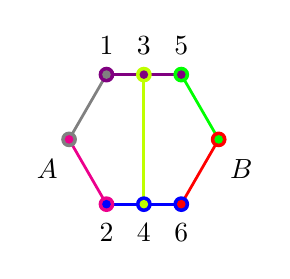
\begin{tikzpicture}  [scale=0.19]
\newdimen\ms
\ms=0.1cm
\tikzstyle{every path}=[line width=1pt]
\tikzstyle{c3}=[circle,inner sep={\ms/8},minimum size=4*\ms]
\tikzstyle{c2}=[circle,inner sep={\ms/8},minimum size=2*\ms]
\tikzstyle{c1}=[circle,inner sep={\ms/8},minimum size=1.1*\ms]
% Radius of regular polygons
\newdimen\R
\newdimen\r
\R=5cm
%\r= { \R * sqrt(3)/2}
% Define positions of all observables
\path
  (0:\R      ) coordinate(1)
  (30:{\R * sqrt(3)/2}      ) coordinate(2)
  (60:\R   ) coordinate(3)
  (90:{\R * sqrt(3)/2}      ) coordinate(4)
  (120:\R  ) coordinate(5)
  (150:{\R * sqrt(3)/2}      ) coordinate(6)
  (180:\R  ) coordinate(7)
  (210:{\R * sqrt(3)/2}      ) coordinate(8)
  (240:\R     ) coordinate(9)
  (270:{\R * sqrt(3)/2}      ) coordinate(10)
  (300:\R        ) coordinate(11)
  (330:{\R * sqrt(3)/2}      ) coordinate(12)
  (0,0      ) coordinate(13)
;
% draw contexts
\draw [color=green] (1) -- (2) -- (3);
\draw [color=violet] (3) -- (4) -- (5);
\draw [color=gray] (5) -- (6) -- (7);
\draw [color=magenta] (7) -- (8) -- (9);
\draw [color=blue] (9) -- (10) -- (11);
\draw [color=red] (11) -- (12) -- (1) ;
\draw [color=lime] (4) -- (13) -- (10);
% draw atoms
\draw (1) coordinate[c2,fill=red,label=275:$B$];
\draw (1) coordinate[c1,fill=green];
%
%NE \draw (2) coordinate[c1,fill=green];
%
\draw (3) coordinate[c2,fill=green,label=90:$5$];
\draw (3) coordinate[c1,fill=violet];
%
\draw (4) coordinate[c2,fill=lime,label=90:$3$];
\draw (4) coordinate[c1,fill=violet];
%
\draw (5) coordinate[c2,fill=violet,label=90:$1$];
\draw (5) coordinate[c1,fill=gray];
%
%NE \draw (6) coordinate[c1,fill=gray];
%
\draw (7) coordinate[c2,fill=gray,label=265:$A$];
\draw (7) coordinate[c1,fill=magenta];
%
%NE \draw (8) coordinate[c1,fill=magenta];
%
\draw (9) coordinate[c2,fill=magenta,label=270:$2$];
\draw (9) coordinate[c1,fill=blue];
%
\draw (10) coordinate[c2,fill=blue,label=270:$4$];
\draw (10) coordinate[c1,fill=lime];
%
\draw (11) coordinate[c2,fill=blue,label=270:$6$];
\draw (11) coordinate[c1,fill=red];
%
%NE \draw (12) coordinate[c1,fill=red];
%
%NE \draw (13) coordinate[c1,fill=lime];
\end{tikzpicture}
&  %%%%%%%%%%%%%%%%%%%%%%%%%%%%%%%%%%%%%%%%%%%%%%%%%%%%%%%%%%%%%%%%%%%%%%%%%%%%%%%%%%%%%%%%%%%%%%%%%%%%%%%%
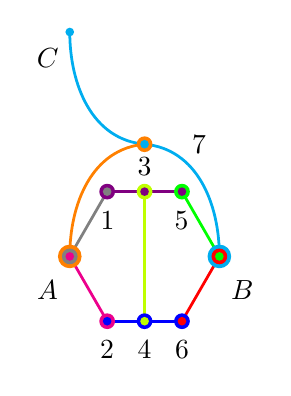
\begin{tikzpicture}  [scale=0.19]
\newdimen\ms
\ms=0.1cm
\tikzstyle{every path}=[line width=1pt]
\tikzstyle{c3}=[circle,inner sep={\ms/8},minimum size=3*\ms]
\tikzstyle{c2}=[circle,inner sep={\ms/8},minimum size=2*\ms]
\tikzstyle{c1}=[circle,inner sep={\ms/8},minimum size=1.1*\ms]
% Radius of regular polygons
\newdimen\R
\R=5cm
%\r= { \R * sqrt(3)/2}
% Define positions of all observables
\path
  (0:\R      ) coordinate(1)
  (30:{\R * sqrt(3)/2}      ) coordinate(2)
  (60:\R   ) coordinate(3)
  (90:{\R * sqrt(3)/2}      ) coordinate(4)
  (120:\R  ) coordinate(5)
  (150:{\R * sqrt(3)/2}      ) coordinate(6)
  (180:\R  ) coordinate(7)
  (210:{\R * sqrt(3)/2}      ) coordinate(8)
  (240:\R     ) coordinate(9)
  (270:{\R * sqrt(3)/2}      ) coordinate(10)
  (300:\R        ) coordinate(11)
  (330:{\R * sqrt(3)/2}      ) coordinate(12)
  (0,0      ) coordinate(13)
  (0,7.5      ) coordinate(14)
  (-5, 15     ) coordinate(15)
  (5, 15     ) coordinate(16)
;
% draw contexts
\draw [color=green] (1) -- (2) -- (3);
\draw [color=violet] (3) -- (4) -- (5);
\draw [color=gray] (5) -- (6) -- (7);
\draw [color=magenta] (7) -- (8) -- (9);
\draw [color=blue] (9) -- (10) -- (11);
\draw [color=red] (11) -- (12) -- (1) ;
\draw [color=lime] (4) -- (13) -- (10);
\draw [color=cyan] (1)   to [out=90,in=355](14)  to [out=175,in=270]  (15);
\draw [color=orange] (7)   to [out=90,in=185] (14); %NE   to [out=5,in=270] (16);
%
% draw atoms
%
%\draw (19) coordinate[c3,fill=teal];
\draw (1) coordinate[c3,fill=cyan,label=275:$B$];
\draw (1) coordinate[c2,fill=red];
\draw (1) coordinate[c1,fill=green];
%
%NE \draw (2) coordinate[c1,fill=green];
%
\draw (3) coordinate[c2,fill=green,label=268:$5$];
\draw (3) coordinate[c1,fill=violet];
%
\draw (4) coordinate[c2,fill=lime];
\draw (4) coordinate[c1,fill=violet,label=90:$3$];
%
\draw (5) coordinate[c2,fill=violet,label=272:$1$];
\draw (5) coordinate[c1,fill=gray];
%
%NE \draw (6) coordinate[c1,fill=gray];
%
\draw (7) coordinate[c3,fill=orange,label=265:$A$];
\draw (7) coordinate[c2,fill=gray];
\draw (7) coordinate[c1,fill=magenta];
%
%NE \draw (8) coordinate[c1,fill=magenta];
%
\draw (9) coordinate[c2,fill=magenta,label=270:$2$];
\draw (9) coordinate[c1,fill=blue];
%
\draw (10) coordinate[c2,fill=blue,label=270:$4$];
\draw (10) coordinate[c1,fill=lime];
%
\draw (11) coordinate[c2,fill=blue,label=270:$6$];
\draw (11) coordinate[c1,fill=red];
%
%NE \draw (12) coordinate[c1,fill=red];
%
%NE \draw (13) coordinate[c1,fill=lime];
%
\draw (14) coordinate[c2,fill=orange,label=0:$\quad 7$];
\draw (14) coordinate[c1,fill=cyan];
%
%
\draw (15) coordinate[c1,fill=cyan,label=265:$C$];
%
%NE \draw (16) coordinate[c1,fill=orange];
%
\end{tikzpicture}
&  %%%%%%%%%%%%%%%%%%%%%%%%%%%%%%%%%%%%%%%%%%%%%%%%%%%%%%%%%%%%%%%%%%%%%%%%%%%%%%%%%%%%%%%%%%%%%%%%%%%
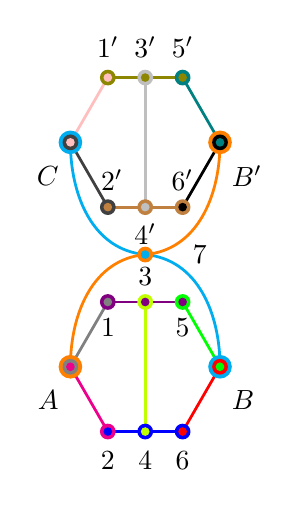
\begin{tikzpicture}  [scale=0.19]
\newdimen\ms
\ms=0.1cm
\tikzstyle{every path}=[line width=1pt]
\tikzstyle{c3}=[circle,inner sep={\ms/8},minimum size=3*\ms]
\tikzstyle{c2}=[circle,inner sep={\ms/8},minimum size=2*\ms]
\tikzstyle{c1}=[circle,inner sep={\ms/8},minimum size=1.1*\ms]
% Radius of regular polygons
\newdimen\R
\R=5cm
%\r= { \R * sqrt(3)/2}
% Define positions of all observables
\path
  (0:\R      ) coordinate(1)
  (30:{\R * sqrt(3)/2}      ) coordinate(2)
  (60:\R   ) coordinate(3)
  (90:{\R * sqrt(3)/2}      ) coordinate(4)
  (120:\R  ) coordinate(5)
  (150:{\R * sqrt(3)/2}      ) coordinate(6)
  (180:\R  ) coordinate(7)
  (210:{\R * sqrt(3)/2}      ) coordinate(8)
  (240:\R     ) coordinate(9)
  (270:{\R * sqrt(3)/2}      ) coordinate(10)
  (300:\R        ) coordinate(11)
  (330:{\R * sqrt(3)/2}      ) coordinate(12)
  (0,0      ) coordinate(13)
  (0,7.5      ) coordinate(14)
  (-5, 15     ) coordinate(15)
  (5, 15     ) coordinate(16)
;
% draw contexts
\draw [color=green] (1) -- (2) -- (3);
\draw [color=violet] (3) -- (4) -- (5);
\draw [color=gray] (5) -- (6) -- (7);
\draw [color=magenta] (7) -- (8) -- (9);
\draw [color=blue] (9) -- (10) -- (11);
\draw [color=red] (11) -- (12) -- (1) ;
\draw [color=lime] (4) -- (13) -- (10);
\draw [teal] ([yshift=15cm]1) -- ([yshift=15cm]2) -- ([yshift=15cm]3);
\draw [olive] ([yshift=15cm]3) -- ([yshift=15cm]4) -- ([yshift=15cm]5);
\draw [pink] ([yshift=15cm]5) -- ([yshift=15cm]6) -- ([yshift=15cm]7);
\draw [darkgray] ([yshift=15cm]7) -- ([yshift=15cm]8) -- ([yshift=15cm]9);
\draw [brown] ([yshift=15cm]9) -- ([yshift=15cm]10) -- ([yshift=15cm]11);
\draw [black] ([yshift=15cm]11) -- ([yshift=15cm]12) -- ([yshift=15cm]1) ;
\draw [lightgray] ([yshift=15cm]4) -- ([yshift=15cm]13) -- ([yshift=15cm]10);
\draw [color=cyan] (1)   to [out=90,in=355](14)  to [out=175,in=270]  (15);
\draw [color=orange] (7)   to [out=90,in=185] (14)  to [out=5,in=270] (16);
%
% draw atoms
%
\draw (1) coordinate[c3,fill=cyan,label=275:$B$];
\draw (1) coordinate[c2,fill=red];
\draw (1) coordinate[c1,fill=green];
%
%NE \draw (2) coordinate[c1,fill=green];
%
\draw (3) coordinate[c2,fill=green];
\draw (3) coordinate[c1,fill=violet,label=268:$5$];
%
\draw (4) coordinate[c2,fill=lime];
\draw (4) coordinate[c1,fill=violet,label=90:$3$];
%
\draw (5) coordinate[c2,fill=violet];
\draw (5) coordinate[c1,fill=gray,label=272:$1$];
%
%NE \draw (6) coordinate[c1,fill=gray];
%
\draw (7) coordinate[c3,fill=orange,label=265:$A$];
\draw (7) coordinate[c2,fill=gray];
\draw (7) coordinate[c1,fill=magenta];
%
%NE \draw (8) coordinate[c1,fill=magenta];
%
\draw (9) coordinate[c2,fill=magenta,label=270:$2$];
\draw (9) coordinate[c1,fill=blue];
%
\draw (10) coordinate[c2,fill=blue,label=270:$4$];
\draw (10) coordinate[c1,fill=lime];
%
\draw (11) coordinate[c2,fill=blue,label=270:$6$];
\draw (11) coordinate[c1,fill=red];
%
%NE \draw (12) coordinate[c1,fill=red];
%
%NE \draw (13) coordinate[c1,fill=lime];
%
\draw (14) coordinate[c2,fill=orange,label=0:$\quad 7$];
\draw (14) coordinate[c1,fill=cyan];
%
%
\draw ([yshift=15cm]1) coordinate[c3,fill=orange,label=275:$B'$];
\draw ([yshift=15cm]1) coordinate[c2,fill=black];
\draw ([yshift=15cm]1) coordinate[c1,fill=teal];
%
%NE \draw ([yshift=15cm]2) coordinate[c1,fill=teal];
%
\draw ([yshift=15cm]3) coordinate[c2,fill=teal,label=90:$5'$];
\draw ([yshift=15cm]3) coordinate[c1,fill=olive];
%
\draw ([yshift=15cm]4) coordinate[c2,fill=lightgray,label=90:$3'$];
\draw ([yshift=15cm]4) coordinate[c1,fill=olive];
%
\draw ([yshift=15cm]5) coordinate[c2,fill=olive,label=90:$1'$];
\draw ([yshift=15cm]5) coordinate[c1,fill=pink];
%
%NE \draw ([yshift=15cm]6) coordinate[c1,fill=pink];
%
\draw ([yshift=15cm]7) coordinate[c3,fill=cyan,label=265:$C$];
\draw ([yshift=15cm]7) coordinate[c2,fill=darkgray];
\draw ([yshift=15cm]7) coordinate[c1,fill=pink];
%
%NE \draw ([yshift=15cm]8) coordinate[c1,fill=darkgray];
%
\draw ([yshift=15cm]9) coordinate[c2,fill=darkgray];
\draw ([yshift=15cm]9) coordinate[c1,fill=brown,label=88:$\;2'$];
%
\draw ([yshift=15cm]10) coordinate[c2,fill=brown];
\draw ([yshift=15cm]10) coordinate[c1,fill=lightgray,label=270:$4'$];
%
\draw ([yshift=15cm]11) coordinate[c2,fill=brown];
\draw ([yshift=15cm]11) coordinate[c1,fill=black,label=92:$6'$];
%
%NE \draw ([yshift=15cm]12) coordinate[c1,fill=black];
%
%NE \draw ([yshift=15cm]13) coordinate[c1,fill=lightgray];
\end{tikzpicture}
\\
(a)&(b)&(c)
\end{tabular}
\end{center}
\caption{\label{Fig1}
(Color online)
Orthogonality diagram of the simplest known~\cite{KS67,Pitowsky2003395,pitowsky-06,pulmannova-91,svozil-tkadlec,tkadlec-96}
(a)~TIFS,  (b)~TITS, and (c)~NSS in $d=3$.
\karl{Points represent propositions, smooth lines represent complete sets
(i.e., one and only one of the propositions must be true); in particular, they indicate
that any pair of propositions connected by a smooth line cannot both be true (exclusiveness).}
\karl{(a)~If $A$ is true then $B$ is false~\cite[Fig.~1, p.~182]{code2}.
(b)~If $A$ is true then $C$ is true~\cite[$\Gamma_1$]{KS67}.
(c)~$A$ and $C$ can only be both true or both false~\cite[$\Gamma_3$]{KS67}.
These sets are realizable in  $S^2$ by taking,
for instance~\cite[p.~206, Fig.~1]{tkadlec-96},
$A     = (    1,\sqrt{2},0     )/\sqrt{3}$,
$v_1     = (   \sqrt{2},-1,1     )/2$,
$v_2     = (   \sqrt{2},-1,-1     )/2$,
$v_3     = (    0,1,1     )/\sqrt{2}$,
$v_4     = (    0,1,-1     )/\sqrt{2}$,
$v_5     = (   \sqrt{2},1,-1     )/2$,
$v_6     = (   \sqrt{2},1,1     )/2$,
$B   = (    -1,\sqrt{2},0     )/\sqrt{3}$,
$v_7          = (    0,0,1     ) $,
$C     = (   \sqrt{2},1,0     )/\sqrt{3} $,
%$b_{2}     = (1, -\sqrt{2}, -3 ) $,
$v_{1'}     = (    -1,\sqrt{2},-1     )/2 $,
$v_{2'}     = (    -1,\sqrt{2},1     )/2 $,
$v_{3'}     = (    1,0,-1     )/\sqrt{2} $,
$v_{4'}     = (    1,0,1     )/\sqrt{2} $,
$v_{5'}     = (    1,\sqrt{2},1     )/2 $,
%$b_{6}     = (1, \sqrt{2}, -3 ) $,
%$b_{7}     = (   \sqrt{2},-1,0     ) $,
%$b_{8}     = (1, \sqrt{2}, 3 ) $,
$v_{6'}     = (    1,\sqrt{2},-1     )/2 $.
%$b_{12}     = (-1, \sqrt{2}, -3 ) $,
%$b_{13}     = (    0,1,0     ) $,
In QT, the proposition $v_i$ is represented by the projector $| v_i \rangle\langle v_i |$.
}
To obtain a \karl{TIFS, TITS and NSS in $d=4$ it}
is enough to add \karl{$\langle v| = (0,0,0,1)$}, and \karl{similarly to obtain TITSes} in higher dimensions.}
\end{figure}

\karl{We define
(i) a {\em true-implies-false set} (TIFS),
(ii) a {\em true-implies-true set} (TITS),
and
(iii) a {\em nonseparating set} (NSS)
as a set $S$ of propositions represented in
QT by rank-one projection operators (or the vectors onto which they project) such that,
due to the exclusiveness and completeness of some of the elements of $S$,
when outcome noncontextuality is assumed,
if proposition $A \in S$ is true,
then a nonexclusive proposition
(i)
$B \in S$  must be false,
(ii)
$C \in S$  must be true as well,
and
(iii)  $C \in S$ must be true, as well as {\it vice versa}, whenever  $C \in S$ is true, then $A$ must be true; i.e.,
$A$ and $C$ cannot be separated with classical probabilities.
This is not the same as in (ii), as for (ii) $v(C)=1$  does not imply $v(A)=1$ (in particular, $v(A)=0$ is allowed).
Explicit examples for the cases (i--iii) are shown in Fig.~\ref{Fig1}(a--c), respectively.}
A {\karl TIFS, TITS, or NSS} $S$ is said to be {\em critical}
if the set resulting from removing any element of $S$ is not a {\karl TIFS, TITS, or NSS, respectively.}

\meil{HISTORY? Upon going through Clifton's paper cited I
found two early instances of TITS different from KS:
Belinfante~\cite[Fig.~C.l. p.~67]{Belinfante-73}, Pitowsky~\cite[p.~394]{Pitowsky-1982-subs}}
\karllate{
Early examples of TIFS have been discussed in
Refs.~\cite[Fig.~1, p.~182]{kochen2},
\cite[Fig.~B.l. p.~64]{Belinfante-73},
\cite[p.~588-589]{stairs83},
\cite[Sects.~IV, Fig.~2]{clifton-93},
\cite[p.~39, Fig.~2.4.6]{pulmannova-91},
and \cite{Pitowsky2003395,pitowsky-06}.
Early examples of TITS can be found in
Refs.~\cite[$\Gamma_1$, p.~86]{kochen1},
\cite[Fig.~C.l. p.~67]{Belinfante-73},
\cite[p.~394]{Pitowsky-1982-subs},
\cite{clifton-93,Johansen-1994,Vermaas-1994},
and~\cite[Lemma~1]{Cabello-1996-bks-fd}.
A NNS is discussed in the KS paper~\cite[$\Gamma_3$, p.~70]{kochen1}.
}



\karl{Any  TIFS, TITS, or NSS}
proves quantum contextuality (i.e., the impossibility of explaining QT with models satisfying outcome noncontextuality)
because for a system prepared in the quantum state in which proposition $A$ is true
there is a nonzero probability of finding proposition \karl{$B$ or $C$ true, false, and different, respectively.}
This is the method followed in the proofs of quantum contextuality proposed by Stairs \cite{code5}, Clifton \cite{code6}, and Cabello et al. \cite{code7,code7b}). All these proofs can be converted into experimental tests of whether nature can be described with noncontextual hidden variable theories \cite{code8}.

\karl{TITSes} also serve to prove state-independent quantum contextuality, i.e., quantum contextuality for any initial quantum state of a quantum system of a given dimension $d \ge 3$. A proof of this can be obtained by concatenating several \karl{TITSes}. This is the method followed by Bell \cite{code3} and Kochen and Specker (KS) \cite{code4} to prove state-independent quantum contextuality in $d=3$. The same method can be extended to any $d \ge 3$ \cite{code9}. State-independent proofs of quantum contextuality have been recently converted into quantum state-independent experimental tests of contextuality \cite{code10, code11, code12, code13, code14, code14b, code14c}.

TITS in which proposition $A$ corresponds to an entangled state and the rest corresponds to product states can be used to prove quantum nonlocality (i.e., the impossibility of explaining QT with local hidden variable theories). This is exactly what is behind Hardy-like proofs of quantum nonlocality \cite{code14d, code14e} (for a detailed explanation, see Refs.~\cite{code14f, code14g}).


\karl{These sets, and, in particular, NSS, are interesting because they demonstrate
a growing deviation from nonclassicality {\em below} the KS theorem:
there still exist classical valuations and truth tables, but they get ``more pathologic''
up to the point where propositional structures with NSS cannot
be ``embedded''~\cite{KS67} into any kind of hidden parameter model, such as partition logics~\cite{svozil-2001-eua},
and their model realizations as Wright's generalized urn model~\cite{wright} or automaton logic~\cite{schaller-96}
(still allowing logics with TIFS or TITS).}

\karl{TITSes} are known for any physical system described by a Hilbert space of dimension $d \ge 2$ \cite{code2, code3, code4}. In $d=3$, Bell found one with $n= 13$ propositions \cite{code3}, and KS found one with $n=10$ \cite{code2, code3, code4}, which is illustrated in Fig.~\ref{Fig1}. Both Bell's and KS's sets belong to a broader family with $n=10+3m$, with $m=0,1,\ldots$ \cite{code7}. For $d>3$, TITS with $n=7+d$ are easy to construct from the set of Fig.~\ref{Fig1} by adding the vector with all components zero but the one corresponding to the new dimension \cite{code9}.

An important question is which are the {\em simplest} \karl{TIFSes, TITSes and NSSes} for any $d \ge 3$, i.e., those with a minimum number of propositions. This is the problem we address in this paper.

%%%%%%%%%%%%%%%%%%%%%%%%%%%%%%%%%%%%%%%%%%%%%%%%%%%%%%%%%%%%%%%%%%%

\section{Method to obtain TITS with minimum number of propositions}

%%%%%%%%%%%%%%%%%%%%%%%%%%%%%%%%%%%%%%%%%%%%%%%%%%%%%%%%%%%%%%%%%%%

\jr{QUIZAS HAYA QUE RECONSTRUIR TODA LA ESTRUCTURA DE SECCIONES}

A TITS can be represented by a graph in which vertices represent propositions, edges connect exclusive propositions,
and \jr{$d$-cliques (}$d$ mutually connected vertices\jr{)} represent complete contexts. A graph is said to be \emph{nonrealizable}
in dimension $d$ if it represents a set of rays (i.e., unit vectors) which is not realizable in $S^{d-1}.$

%%%%%%%%%%%%%%%%%%%%%%%%%%%%%%%%%%%%%%%%%%%%%%%%%%%%%%%%%%%%%%%%%%%

{\em Lemma 1:~}\cite{code21,SP15} The simplest nonrealizable graph in $d=1$ consists of two vertices.
The simplest nonrealizable graph in $d=2$ has three vertices with one of them connected to the other two.
From these to nonrealizable graphs one can recursively construct nonrealizable graphs
in any dimension $d$ by starting from the nonrealizable graph in dimension $d-2$
and adding to it two vertices connected with all vertices of the nonrealizable graph in $d-2$.

%%%%%%%%%%%%%%%%%%%%%%%%%%%%%%%%%%%%%%%%%%%%%%%%%%%%%%%%%%%%%%%%%%%

\jr{THIS PROOF IS IN THE CITES  \sout{
{\em Proof:} One cannot have two different ways in $S^0$ because there is only one ray in $S^0$. In $S^1$, if a ray is orthogonal to a second ray, and the second is orthogonal to the third, then the first and third ray should be the same. If we add two dimensions and two different rays, both orthogonal to those of previous set $I$, then these two new rays span a two-dimensional subspace orthogonal to $I$. Therefore, if $I$ was nonrealizable, then the resulting set is also nonrealizable.\endproof} }

%%%%%%%%%%%%%%%%%%%%%%%%%%%%%%%%%%%%%%%%%%%%%%%%%%%%%%%%%%%%%%%%%%%

{\em Lemma 2:} Every $n$-vertex graph corresponding to a critical TITS in dimension $d$ contains an ($n+1-d$)-vertex graph corresponding to a TIFS.

%%%%%%%%%%%%%%%%%%%%%%%%%%%%%%%%%%%%%%%%%%%%%%%%%%%%%%%%%%%%%%%%%%%

{\em Proof:} Let be $G$ a graph corresponding to a TITS, then $b \in K_d$ is true and any adjacent $v$ must be false. Then the subgraph taken from the other true $a$ to false $v$ forms a TIFS. Moreover, any $v_i \in K_d-1$ can be taken as false to get a TIFS. \endproof

%%%%%%%%%%%%%%%%%%%%%%%%%%%%%%%%%%%%%%%%%%%%%%%%%%%%%%%%%%%%%%%%%%%

{\em Lemma 3:} The graph of a critical TIFS must be biconnected (i.e., when removing any vertex the resulting graph must be still connected).

%%%%%%%%%%%%%%%%%%%%%%%%%%%%%%%%%%%%%%%%%%%%%%%%%%%%%%%%%%%%%%%%%%%

{\em Proof:} Suppose it is not. Cut vertex split graph in two connected components, if true and false vertices are in the same component, then the graph is not critical and if true and \jr{false} vertices are in different components then cut vertex can substitute anyone of them getting a smaller TIFS. \endproof


%%%%%%%%%%%%%%%%%%%%%%%%%%%%%%%%%%%%%%%%%%%%%%%%%%%%%%%%%%%%%%%%%%%
%\jr{As consecuence of the Lemma 3, Every vertex of a graph corresponding to a TIFS must be connected to, at least, two vertices (i.e., the graph must have minimal valency two).}

{\em Corollary 1:} Every vertex of a graph corresponding to a TIFS must be connected to, at least, two vertices (i.e., the graph must have minimal valency two).

%%%%%%%%%%%%%%%%%%%%%%%%%%%%%%%%%%%%%%%%%%%%%%%%%%%%%%%%%%%%%%%%%%%

{\em Proof:} Directly from Lemma 3. \endproof

%%%%%%%%%%%%%%%%%%%%%%%%%%%%%%%%%%%%%%%%%%%%%%%%%%%%%%%%%%%%%%%%%%%

{\em Lemma 4:} Every TIFS graph in dimension $d$ contains, at least, two $K_d$ graphs.

%%%%%%%%%%%%%%%%%%%%%%%%%%%%%%%%%%%%%%%%%%%%%%%%%%%%%%%%%%%%%%%%%%%

{\em Proof:} %\jr{(FIGURE? NO ME ACABA DE CONVENCER ESTA PRUEBA)}
 Let be $G$ a TIFS graph with true vertex $a$ and false vertex $b$.
$G$ is not trivial TIFS, so there is another true vertex $x$ linked to b and other $d-1$ vertices.
\jr{\sout{Let be $C$ the rest of vertices in $G$ (except $a$ and $b$).}} %\jr{hay que redactarlo entero otra vez}
We consider two different cases.
a) Every vertex in \jr{$V(G)-\{a,b,x\}$} belongs to $N(a)$ and $b$ is linked to $C$.
Note that in this case $a \cup N(a)$ and $b \cup N(b)$ form two $K_d$'s.
b) Only several vertices in \jr{$V(G)-\{a,b,x\}$} belongs to $N(a)$.
We have a set of vertices in \jr{$V(G)-\{a,b,x\}$}with value false,
but such vertices are not linked directly to $a$,
so their value must be forced through another true vertex \jr{\sout{out $C$}}.
This vertex is not linked to $a$, so it has to belong to a context, i.e. a $K_d$.\endproof

%%%%%%%%%%%%%%%%%%%%%%%%%%%%%%%%%%%%%%%%%%%%%%%%%%%%%%%%%%%%%%%%%%%

%\jr{EL ENUNCIADO DEL SIGUIENTE LEMA ES CONFUSO. SE PRUEBA QUE EL GRAFO ES MÍNIMO}

\jr{\sout{{\em Lemma 5:} The graph of any 8-vertex TIFS in $d=3$ must contain at least two triangles.}}

%%%%%%%%%%%%%%%%%%%%%%%%%%%%%%%%%%%%%%%%%%%%%%%%%%%%%%%%%%%%%%%%%%%

\jr{\sout{{\em Proof:} From Lemma 4. Otherwise the graph can be colored as follows: first vertex $a$ true and everything else false. \endproof}}

%%%%%%%%%%%%%%%%%%%%%%%%%%%%%%%%%%%%%%%%%%%%%%%%%%%%%%%%%%%%%%%%%%%

\section{Dimension 3 - Specker bug}

\jr{CHANGED SECTIONS ORDER}

Therefore, we have a method to obtain the minimal TITS in $d=3$ \karllate{which proceeds as follows:}

{\em Step 1:} We generate all nonisomorphic $n$-vertex biconnected graphs \jr{(Lemma 3)} of minimal valence two  \jr{(Corollary 1)},
not containing cycles on length four  \jr{(Lemma 1)} and containing at least two triangles  \jr{(Lemma 4)} \jr{for $n$ less or equal than $8$}.
This can be efficiently done using the computer program {\em nauty} \cite{code15}.
We obtain that there are 2 \karllate{such} graphs for $n=7$, and 8 graphs for $n=8$. All of them are illustrated in Fig.~\ref{Fig2}.

%%%%%%%%%%%%%%%%%%%%%%%%%%%%%%%%%%%%%%%%%%%%%%%%%%%%%%%%%%%%%%%%%%%
% Fig. 2
%%%%%%%%%%%%%%%%%%%%%%%%%%%%%%%%%%%%%%%%%%%%%%%%%%%%%%%%%%%%%%%%%%%
\begin{figure}
\begin{center}
\setlength{\tabcolsep}{1em}
\begin{tabular}{ccccc}
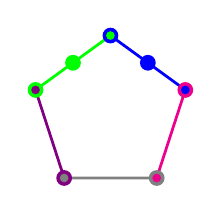
\begin{tikzpicture}  [scale=0.20]
\newdimen\ms
\ms=0.1cm
\tikzstyle{every path}=[line width=1pt]
\tikzstyle{c3}=[circle,inner sep={\ms/8},minimum size=3*\ms]
\tikzstyle{c2}=[circle,inner sep={\ms/8},minimum size=2*\ms]
\tikzstyle{c1}=[circle,inner sep={\ms/8},minimum size=1.1*\ms]
% Radius of regular polygons
\newdimen\R
\R=5cm
% Define positions of all observables
\path
  ({90 + 0 * 360 /5}:\R      ) coordinate(1)
  ({90 + 360 /10 + 0 * 360/5} : {\R * 0.6881/0.8507} ) coordinate(2)
  ({90 + 1 * 360 /5}:\R   ) coordinate(3)
  ({90 + 360 /10 + 1 * 360/5} : {\R * 0.6881/0.8507} ) coordinate(4)
  ({90 + 2 * 360 /5}:\R  ) coordinate(5)
  ({90 + 360 /10 + 2 * 360/5} : {\R * 0.6881/0.8507} ) coordinate(6)
  ({90 + 3 * 360 /5}:\R  ) coordinate(7)
  ({90 + 360 /10 + 3 * 360/5} : {\R * 0.6881/0.8507} ) coordinate(8)
  ({90 + 4 * 360 /5}:\R     ) coordinate(9)
  ({90 + 360 /10 + 4 * 360/5} : {\R * 0.6881/0.8507} ) coordinate(10)
  (0,0      ) coordinate(13);
% draw contexts
\draw [color=green] (1) -- (2) -- (3);
\draw [color=violet] (3) -- (4) -- (5);
\draw [color=gray] (5) -- (6) -- (7);
\draw [color=magenta] (7) -- (8) -- (9);
\draw [color=blue] (9) -- (10) -- (1);
%
%%
%% draw atoms
%%
%
 \draw (1) coordinate[c2,fill=blue];
 \draw (1) coordinate[c1,fill=green];
%%
 \draw (2) coordinate[c2,fill=green];
%%
 \draw (3) coordinate[c2,fill=green];
 \draw (3) coordinate[c1,fill=violet];
 \draw (5) coordinate[c2,fill=violet];
 \draw (5) coordinate[c1,fill=gray];
 \draw (7) coordinate[c2,fill=gray];
 \draw (7) coordinate[c1,fill=magenta];
 \draw (9) coordinate[c2,fill=magenta];
 \draw (9) coordinate[c1,fill=blue];
\draw (10) coordinate[c2,fill=blue];
\end{tikzpicture}
&   %%%%%%%%%%%%%%%%%%%%%%%%%%%%%%%%%%%%%%%%%%%%%%%%%%%%%%%%%%%%%%%%%%%%%%%%%%%%%%%%%%%%%%%%%%%%%%%%%
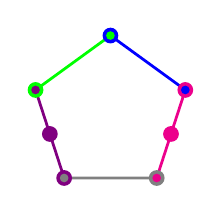
\begin{tikzpicture}  [scale=0.20]
\newdimen\ms
\ms=0.1cm
\tikzstyle{every path}=[line width=1pt]
\tikzstyle{c3}=[circle,inner sep={\ms/8},minimum size=3*\ms]
\tikzstyle{c2}=[circle,inner sep={\ms/8},minimum size=2*\ms]
\tikzstyle{c1}=[circle,inner sep={\ms/8},minimum size=1.1*\ms]
% Radius of regular polygons
\newdimen\R
\R=5cm
%\r= { \R * sqrt(3)/2}
% Define positions of all observables
\path
  ({90 + 0 * 360 /5}:\R      ) coordinate(1)
  ({90 + 360 /10 + 0 * 360/5} : {\R * 0.6881/0.8507} ) coordinate(2)
  ({90 + 1 * 360 /5}:\R   ) coordinate(3)
  ({90 + 360 /10 + 1 * 360/5} : {\R * 0.6881/0.8507} ) coordinate(4)
  ({90 + 2 * 360 /5}:\R  ) coordinate(5)
  ({90 + 360 /10 + 2 * 360/5} : {\R * 0.6881/0.8507} ) coordinate(6)
  ({90 + 3 * 360 /5}:\R  ) coordinate(7)
  ({90 + 360 /10 + 3 * 360/5} : {\R * 0.6881/0.8507} ) coordinate(8)
  ({90 + 4 * 360 /5}:\R     ) coordinate(9)
  ({90 + 360 /10 + 4 * 360/5} : {\R * 0.6881/0.8507} ) coordinate(10)
  (0,0      ) coordinate(13);
% draw contexts
\draw [color=green] (1) -- (2) -- (3);
\draw [color=violet] (3) -- (4) -- (5);
\draw [color=gray] (5) -- (6) -- (7);
\draw [color=magenta] (7) -- (8) -- (9);
\draw [color=blue] (9) -- (10) -- (1);
%
%%
%% draw atoms
%%
%
%\draw (1) coordinate[c3,fill=cyan];
 \draw (1) coordinate[c2,fill=blue];
 \draw (1) coordinate[c1,fill=green];
%%
%\draw (2) coordinate[c1,fill=green];
%%
 \draw (3) coordinate[c2,fill=green];
 \draw (3) coordinate[c1,fill=violet];
%%
%\draw (4) coordinate[c2,fill=lime];
 \draw (4) coordinate[c2,fill=violet];
%%
 \draw (5) coordinate[c2,fill=violet];
 \draw (5) coordinate[c1,fill=gray];
%%
% \draw (6) coordinate[c1,fill=gray];
%%
 \draw (7) coordinate[c2,fill=gray];
 \draw (7) coordinate[c1,fill=magenta];
%%
 \draw (8) coordinate[c2,fill=magenta];
%%
 \draw (9) coordinate[c2,fill=magenta];
 \draw (9) coordinate[c1,fill=blue];
\end{tikzpicture}
\\  %%%%%%%%%%%%%%%%%%%%%%%%%%%%%%%%%%%%%%%%%%%%%%%%%%%%%%%%%%%%%%%%%%%%%%%%%%%%%%%%%%%%%%%%%%%%%%%%%
\\  %%%%%%%%%%%%%%%%%%%%%%%%%%%%%%%%%%%%%%%%%%%%%%%%%%%%%%%%%%%%%%%%%%%%%%%%%%%%%%%%%%%%%%%%%%%%%%%%%
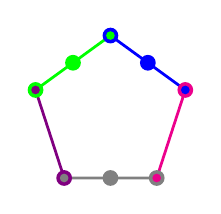
\begin{tikzpicture}  [scale=0.20]
\newdimen\ms
\ms=0.1cm
\tikzstyle{every path}=[line width=1pt]
\tikzstyle{c3}=[circle,inner sep={\ms/8},minimum size=3*\ms]
\tikzstyle{c2}=[circle,inner sep={\ms/8},minimum size=2*\ms]
\tikzstyle{c1}=[circle,inner sep={\ms/8},minimum size=1.1*\ms]

% Radius of regular polygons
\newdimen\R
\R=5cm
% Define positions of all observables
\path
  ({90 + 0 * 360 /5}:\R      ) coordinate(1)
  ({90 + 360 /10 + 0 * 360/5} : {\R * 0.6881/0.8507} ) coordinate(2)
  ({90 + 1 * 360 /5}:\R   ) coordinate(3)
  ({90 + 360 /10 + 1 * 360/5} : {\R * 0.6881/0.8507} ) coordinate(4)
  ({90 + 2 * 360 /5}:\R  ) coordinate(5)
  ({90 + 360 /10 + 2 * 360/5} : {\R * 0.6881/0.8507} ) coordinate(6)
  ({90 + 3 * 360 /5}:\R  ) coordinate(7)
  ({90 + 360 /10 + 3 * 360/5} : {\R * 0.6881/0.8507} ) coordinate(8)
  ({90 + 4 * 360 /5}:\R     ) coordinate(9)
  ({90 + 360 /10 + 4 * 360/5} : {\R * 0.6881/0.8507} ) coordinate(10)
  (0,0      ) coordinate(13);
% draw contexts
\draw [color=green] (1) -- (2) -- (3);
\draw [color=violet] (3) -- (4) -- (5);
\draw [color=gray] (5) -- (6) -- (7);
\draw [color=magenta] (7) -- (8) -- (9);
\draw [color=blue] (9) -- (10) -- (1);
%
%%
%% draw atoms
%%
%
 \draw (1) coordinate[c2,fill=blue];
 \draw (1) coordinate[c1,fill=green];
%%
 \draw (2) coordinate[c2,fill=green];
%%
 \draw (3) coordinate[c2,fill=green];
 \draw (3) coordinate[c1,fill=violet];
 \draw (5) coordinate[c2,fill=violet];
 \draw (5) coordinate[c1,fill=gray];
 \draw (6) coordinate[c2,fill=gray];
 \draw (7) coordinate[c2,fill=gray];
 \draw (7) coordinate[c1,fill=magenta];
 \draw (9) coordinate[c2,fill=magenta];
 \draw (9) coordinate[c1,fill=blue];
\draw (10) coordinate[c2,fill=blue];
\end{tikzpicture}
&   %%%%%%%%%%%%%%%%%%%%%%%%%%%%%%%%%%%%%%%%%%%%%%%%%%%%%%%%%%%%%%%%%%%%%%%%%%%%%%%%%%%%%%%%%%%%%%%%%
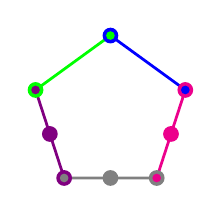
\begin{tikzpicture}  [scale=0.20]
\newdimen\ms
\ms=0.1cm
\tikzstyle{every path}=[line width=1pt]
\tikzstyle{c3}=[circle,inner sep={\ms/8},minimum size=3*\ms]
\tikzstyle{c2}=[circle,inner sep={\ms/8},minimum size=2*\ms]
\tikzstyle{c1}=[circle,inner sep={\ms/8},minimum size=1.1*\ms]
% Radius of regular polygons
\newdimen\R
\R=5cm
%\r= { \R * sqrt(3)/2}
% Define positions of all observables
\path
  ({90 + 0 * 360 /5}:\R      ) coordinate(1)
  ({90 + 360 /10 + 0 * 360/5} : {\R * 0.6881/0.8507} ) coordinate(2)
  ({90 + 1 * 360 /5}:\R   ) coordinate(3)
  ({90 + 360 /10 + 1 * 360/5} : {\R * 0.6881/0.8507} ) coordinate(4)
  ({90 + 2 * 360 /5}:\R  ) coordinate(5)
  ({90 + 360 /10 + 2 * 360/5} : {\R * 0.6881/0.8507} ) coordinate(6)
  ({90 + 3 * 360 /5}:\R  ) coordinate(7)
  ({90 + 360 /10 + 3 * 360/5} : {\R * 0.6881/0.8507} ) coordinate(8)
  ({90 + 4 * 360 /5}:\R     ) coordinate(9)
  ({90 + 360 /10 + 4 * 360/5} : {\R * 0.6881/0.8507} ) coordinate(10)
  (0,0      ) coordinate(13) ;
% draw contexts
\draw [color=green] (1) -- (2) -- (3);
\draw [color=violet] (3) -- (4) -- (5);
\draw [color=gray] (5) -- (6) -- (7);
\draw [color=magenta] (7) -- (8) -- (9);
\draw [color=blue] (9) -- (10) -- (1);
%
%%
%% draw atoms
%%
%
%\draw (1) coordinate[c3,fill=cyan];
 \draw (1) coordinate[c2,fill=blue];
 \draw (1) coordinate[c1,fill=green];
%%
%\draw (2) coordinate[c1,fill=green];
%%
 \draw (3) coordinate[c2,fill=green];
 \draw (3) coordinate[c1,fill=violet];
%%
%\draw (4) coordinate[c2,fill=lime];
 \draw (4) coordinate[c2,fill=violet];
%%
 \draw (5) coordinate[c2,fill=violet];
 \draw (5) coordinate[c1,fill=gray];
%%
 \draw (6) coordinate[c2,fill=gray];
%%
 \draw (7) coordinate[c2,fill=gray];
 \draw (7) coordinate[c1,fill=magenta];
%%
 \draw (8) coordinate[c2,fill=magenta];
%%
 \draw (9) coordinate[c2,fill=magenta];
 \draw (9) coordinate[c1,fill=blue];
\end{tikzpicture}
\end{tabular}
\\
%%%%%%%%%%%%%%%%%%%%%%%%%%%%%%%%%%%%%%%%%%%%%%%%%%%%%%%%%%%%%%%%%%%%%%%%%%%%%%%%%%%%%%%%%%
\begin{tabular}{ccccc}
\\
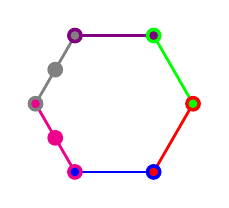
\begin{tikzpicture}  [scale=0.20]
\newdimen\ms
\ms=0.1cm
\tikzstyle{every path}=[line width=1pt]
\tikzstyle{c3}=[circle,inner sep={\ms/8},minimum size=3*\ms]
\tikzstyle{c2}=[circle,inner sep={\ms/8},minimum size=2*\ms]
\tikzstyle{c1}=[circle,inner sep={\ms/8},minimum size=1.1*\ms]
\newdimen\R
\R=5cm
\path
  (0:\R      ) coordinate(1)
  (30:{\R * sqrt(3)/2}      ) coordinate(2)
  (60:\R   ) coordinate(3)
  (90:{\R * sqrt(3)/2}      ) coordinate(4)
  (120:\R  ) coordinate(5)
  (150:{\R * sqrt(3)/2}      ) coordinate(6)
  (180:\R  ) coordinate(7)
  (210:{\R * sqrt(3)/2}      ) coordinate(8)
  (240:\R     ) coordinate(9)
  (270:{\R * sqrt(3)/2}      ) coordinate(10)
  (300:\R        ) coordinate(11)
  (330:{\R * sqrt(3)/2}      ) coordinate(12)
  (0,0      ) coordinate(13);
\draw [color=green] (1) -- (2) -- (3);
\draw [color=violet] (3) -- (4) -- (5);
\draw [color=gray] (5) -- (6) -- (7);
\draw [color=magenta] (7) -- (8) -- (9);
\draw [color=blue] (9) -- (10) -- (11);
\draw [color=red] (11) -- (12) -- (1) ;
 \draw (1) coordinate[c2,fill=red];
 \draw (1) coordinate[c1,fill=green];
 \draw (3) coordinate[c2,fill=green];
 \draw (3) coordinate[c1,fill=violet];
 \draw (5) coordinate[c2,fill=violet];
 \draw (5) coordinate[c1,fill=gray];
 \draw (6) coordinate[c2,fill=gray];
 \draw (7) coordinate[c2,fill=gray];
 \draw (7) coordinate[c1,fill=magenta];
 \draw (8) coordinate[c2,fill=magenta];
 \draw (9) coordinate[c2,fill=magenta];
 \draw (9) coordinate[c1,fill=blue];
 \draw (11) coordinate[c2,fill=blue];
 \draw (11) coordinate[c1,fill=red];
\end{tikzpicture}
&            %%%%%%%%%%%%%%%%%%%%%%%%%%%%%%%%%%%%%%%%%%%%%%%%%%%%%%%%%%%%%%%%%%%%%%%%%%%%%%%%%%%%%%%%%%%%%%%%%
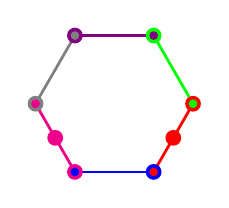
\begin{tikzpicture}  [scale=0.20]
\newdimen\ms
\ms=0.1cm
\tikzstyle{every path}=[line width=1pt]
\tikzstyle{c3}=[circle,inner sep={\ms/8},minimum size=3*\ms]
\tikzstyle{c2}=[circle,inner sep={\ms/8},minimum size=2*\ms]
\tikzstyle{c1}=[circle,inner sep={\ms/8},minimum size=1.1*\ms]
\newdimen\R
\R=5cm
\path
  (0:\R      ) coordinate(1)
  (30:{\R * sqrt(3)/2}      ) coordinate(2)
  (60:\R   ) coordinate(3)
  (90:{\R * sqrt(3)/2}      ) coordinate(4)
  (120:\R  ) coordinate(5)
  (150:{\R * sqrt(3)/2}      ) coordinate(6)
  (180:\R  ) coordinate(7)
  (210:{\R * sqrt(3)/2}      ) coordinate(8)
  (240:\R     ) coordinate(9)
  (270:{\R * sqrt(3)/2}      ) coordinate(10)
  (300:\R        ) coordinate(11)
  (330:{\R * sqrt(3)/2}      ) coordinate(12)
  (0,0      ) coordinate(13);
\draw [color=green] (1) -- (2) -- (3);
\draw [color=violet] (3) -- (4) -- (5);
\draw [color=gray] (5) -- (6) -- (7);
\draw [color=magenta] (7) -- (8) -- (9);
\draw [color=blue] (9) -- (10) -- (11);
\draw [color=red] (11) -- (12) -- (1) ;
 \draw (1) coordinate[c2,fill=red];
 \draw (1) coordinate[c1,fill=green];
 \draw (3) coordinate[c2,fill=green];
 \draw (3) coordinate[c1,fill=violet];
 \draw (5) coordinate[c2,fill=violet];
 \draw (5) coordinate[c1,fill=gray];
 \draw (7) coordinate[c2,fill=gray];
 \draw (7) coordinate[c1,fill=magenta];
 \draw (8) coordinate[c2,fill=magenta];
 \draw (9) coordinate[c2,fill=magenta];
 \draw (9) coordinate[c1,fill=blue];
 \draw (11) coordinate[c2,fill=blue];
 \draw (11) coordinate[c1,fill=red];
 \draw (12) coordinate[c2,fill=red];
\end{tikzpicture}
&            %%%%%%%%%%%%%%%%%%%%%%%%%%%%%%%%%%%%%%%%%%%%%%%%%%%%%%%%%%%%%%%%%%%%%%%%%%%%%%%%%%%%%%%%%%%%%%%%%
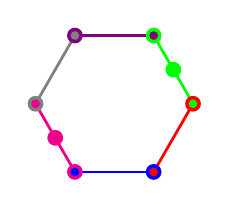
\begin{tikzpicture}  [scale=0.20]
\newdimen\ms
\ms=0.1cm
\tikzstyle{every path}=[line width=1pt]
\tikzstyle{c3}=[circle,inner sep={\ms/8},minimum size=3*\ms]
\tikzstyle{c2}=[circle,inner sep={\ms/8},minimum size=2*\ms]
\tikzstyle{c1}=[circle,inner sep={\ms/8},minimum size=1.1*\ms]
\newdimen\R
\R=5cm
\path
  (0:\R      ) coordinate(1)
  (30:{\R * sqrt(3)/2}      ) coordinate(2)
  (60:\R   ) coordinate(3)
  (90:{\R * sqrt(3)/2}      ) coordinate(4)
  (120:\R  ) coordinate(5)
  (150:{\R * sqrt(3)/2}      ) coordinate(6)
  (180:\R  ) coordinate(7)
  (210:{\R * sqrt(3)/2}      ) coordinate(8)
  (240:\R     ) coordinate(9)
  (270:{\R * sqrt(3)/2}      ) coordinate(10)
  (300:\R        ) coordinate(11)
  (330:{\R * sqrt(3)/2}      ) coordinate(12)
  (0,0      ) coordinate(13);
\draw [color=green] (1) -- (2) -- (3);
\draw [color=violet] (3) -- (4) -- (5);
\draw [color=gray] (5) -- (6) -- (7);
\draw [color=magenta] (7) -- (8) -- (9);
\draw [color=blue] (9) -- (10) -- (11);
\draw [color=red] (11) -- (12) -- (1) ;
 \draw (1) coordinate[c2,fill=red];
 \draw (1) coordinate[c1,fill=green];
 \draw (2) coordinate[c2,fill=green];
 \draw (3) coordinate[c2,fill=green];
 \draw (3) coordinate[c1,fill=violet];
 \draw (5) coordinate[c2,fill=violet];
 \draw (5) coordinate[c1,fill=gray];
 \draw (7) coordinate[c2,fill=gray];
 \draw (7) coordinate[c1,fill=magenta];
\draw (8) coordinate[c2,fill=magenta];
 \draw (9) coordinate[c2,fill=magenta];
 \draw (9) coordinate[c1,fill=blue];
 \draw (11) coordinate[c2,fill=blue];
 \draw (11) coordinate[c1,fill=red];
\end{tikzpicture}
\\            %%%%%%%%%%%%%%%%%%%%%%%%%%%%%%%%%%%%%%%%%%%%%%%%%%%%%%%%%%%%%%%%%%%%%%%%%%%%%%%%%%%%%%%%%%%%%%%%%
\\            %%%%%%%%%%%%%%%%%%%%%%%%%%%%%%%%%%%%%%%%%%%%%%%%%%%%%%%%%%%%%%%%%%%%%%%%%%%%%%%%%%%%%%%%%%%%%%%%%
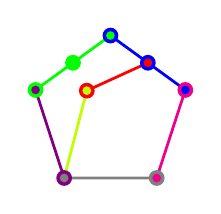
\begin{tikzpicture}  [scale=0.20]
\newdimen\ms
\ms=0.1cm
\tikzstyle{every path}=[line width=1pt]
\tikzstyle{c3}=[circle,inner sep={\ms/8},minimum size=3*\ms]
\tikzstyle{c2}=[circle,inner sep={\ms/8},minimum size=2*\ms]
\tikzstyle{c1}=[circle,inner sep={\ms/8},minimum size=1.1*\ms]
\newdimen\R
\R=5cm
\path
  ({90 + 0 * 360 /5}:\R      ) coordinate(1)
  ({90 + 360 /10 + 0 * 360/5} : {\R * 0.6881/0.8507} ) coordinate(2)
  ({90 + 1 * 360 /5}:\R   ) coordinate(3)
  ({90 + 360 /10 + 1 * 360/5} : {\R * 0.6881/0.8507} ) coordinate(4)
  ({90 + 2 * 360 /5}:\R  ) coordinate(5)
  ({90 + 360 /10 + 2 * 360/5} : {\R * 0.6881/0.8507} ) coordinate(6)
  ({90 + 3 * 360 /5}:\R  ) coordinate(7)
  ({90 + 360 /10 + 3 * 360/5} : {\R * 0.6881/0.8507} ) coordinate(8)
  ({90 + 4 * 360 /5}:\R     ) coordinate(9)
  ({90 + 360 /10 + 4 * 360/5} : {\R * 0.6881/0.8507} ) coordinate(10)
  (-1.5,1.5      ) coordinate(13);
\draw [color=green] (1) -- (2) -- (3);
\draw [color=violet] (3) -- (4) -- (5);
\draw [color=gray] (5) -- (6) -- (7);
\draw [color=magenta] (7) -- (8) -- (9);
\draw [color=blue] (9) -- (10) -- (1);
\draw [color=red] (10) -- (13)  ;
\draw [color=lime] (13) -- (5);
\draw (1) coordinate[c2,fill=blue];
\draw (1) coordinate[c1,fill=green];
\draw (2) coordinate[c2,fill=green];
 \draw (3) coordinate[c2,fill=green];
 \draw (3) coordinate[c1,fill=violet];
 \draw (5) coordinate[c2,fill=violet];
 \draw (5) coordinate[c1,fill=gray];
 \draw (7) coordinate[c2,fill=gray];
 \draw (7) coordinate[c1,fill=magenta];
 \draw (9) coordinate[c2,fill=magenta];
 \draw (9) coordinate[c1,fill=blue];
 \draw (10) coordinate[c2,fill=blue];
 \draw (10) coordinate[c1,fill=red];
 \draw (13) coordinate[c2,fill=red];
 \draw (13) coordinate[c1,fill=lime];
\end{tikzpicture}
&            %%%%%%%%%%%%%%%%%%%%%%%%%%%%%%%%%%%%%%%%%%%%%%%%%%%%%%%%%%%%%%%%%%%%%%%%%%%%%%%%%%%%%%%%%%%%%%%%%
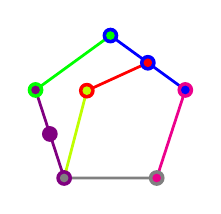
\begin{tikzpicture}  [scale=0.20]
\newdimen\ms
\ms=0.1cm
\tikzstyle{every path}=[line width=1pt]
\tikzstyle{c3}=[circle,inner sep={\ms/8},minimum size=3*\ms]
\tikzstyle{c2}=[circle,inner sep={\ms/8},minimum size=2*\ms]
\tikzstyle{c1}=[circle,inner sep={\ms/8},minimum size=1.1*\ms]
\newdimen\R
\R=5cm
\path
  ({90 + 0 * 360 /5}:\R      ) coordinate(1)
  ({90 + 360 /10 + 0 * 360/5} : {\R * 0.6881/0.8507} ) coordinate(2)
  ({90 + 1 * 360 /5}:\R   ) coordinate(3)
  ({90 + 360 /10 + 1 * 360/5} : {\R * 0.6881/0.8507} ) coordinate(4)
  ({90 + 2 * 360 /5}:\R  ) coordinate(5)
  ({90 + 360 /10 + 2 * 360/5} : {\R * 0.6881/0.8507} ) coordinate(6)
  ({90 + 3 * 360 /5}:\R  ) coordinate(7)
  ({90 + 360 /10 + 3 * 360/5} : {\R * 0.6881/0.8507} ) coordinate(8)
  ({90 + 4 * 360 /5}:\R     ) coordinate(9)
  ({90 + 360 /10 + 4 * 360/5} : {\R * 0.6881/0.8507} ) coordinate(10)
  (-1.5,1.5      ) coordinate(13);
\draw [color=green] (1) -- (2) -- (3);
\draw [color=violet] (3) -- (4) -- (5);
\draw [color=gray] (5) -- (6) -- (7);
\draw [color=magenta] (7) -- (8) -- (9);
\draw [color=blue] (9) -- (10) -- (1);
\draw [color=red] (10) -- (13)  ;
\draw [color=lime] (13) -- (5);
\draw (1) coordinate[c2,fill=blue];
\draw (1) coordinate[c1,fill=green];
 \draw (3) coordinate[c2,fill=green];
 \draw (3) coordinate[c1,fill=violet];
 \draw (4) coordinate[c2,fill=violet];
 \draw (5) coordinate[c2,fill=violet];
 \draw (5) coordinate[c1,fill=gray];
 \draw (7) coordinate[c2,fill=gray];
 \draw (7) coordinate[c1,fill=magenta];
 \draw (9) coordinate[c2,fill=magenta];
 \draw (9) coordinate[c1,fill=blue];
 \draw (10) coordinate[c2,fill=blue];
 \draw (10) coordinate[c1,fill=red];
 \draw (13) coordinate[c2,fill=red];
 \draw (13) coordinate[c1,fill=lime];
\end{tikzpicture}
&            %%%%%%%%%%%%%%%%%%%%%%%%%%%%%%%%%%%%%%%%%%%%%%%%%%%%%%%%%%%%%%%%%%%%%%%%%%%%%%%%%%%%%%%%%%%%%%%%%
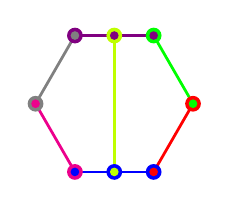
\begin{tikzpicture}  [scale=0.20]
\newdimen\ms
\ms=0.1cm
\tikzstyle{every path}=[line width=1pt]
\tikzstyle{c3}=[circle,inner sep={\ms/8},minimum size=3*\ms]
\tikzstyle{c2}=[circle,inner sep={\ms/8},minimum size=2*\ms]
\tikzstyle{c1}=[circle,inner sep={\ms/8},minimum size=1.1*\ms]
\newdimen\R
\R=5cm
\path
  (0:\R      ) coordinate(1)
  (30:{\R * sqrt(3)/2}      ) coordinate(2)
  (60:\R   ) coordinate(3)
  (90:{\R * sqrt(3)/2}      ) coordinate(4)
  (120:\R  ) coordinate(5)
  (150:{\R * sqrt(3)/2}      ) coordinate(6)
  (180:\R  ) coordinate(7)
  (210:{\R * sqrt(3)/2}      ) coordinate(8)
  (240:\R     ) coordinate(9)
  (270:{\R * sqrt(3)/2}      ) coordinate(10)
  (300:\R        ) coordinate(11)
  (330:{\R * sqrt(3)/2}      ) coordinate(12)
  (0,0      ) coordinate(13);
\draw [color=green] (1) -- (2) -- (3);
\draw [color=violet] (3) -- (4) -- (5);
\draw [color=gray] (5) -- (6) -- (7);
\draw [color=magenta] (7) -- (8) -- (9);
\draw [color=blue] (9) -- (10) -- (11);
\draw [color=red] (11) -- (12) -- (1) ;
\draw [color=lime] (4) -- (13) -- (10);
 \draw (1) coordinate[c2,fill=red];
 \draw (1) coordinate[c1,fill=green];
 %\draw (2) coordinate[c2,fill=green];
 \draw (3) coordinate[c2,fill=green];
 \draw (3) coordinate[c1,fill=violet];
 \draw (4) coordinate[c2,fill=lime];
 \draw (4) coordinate[c1,fill=violet];
 \draw (5) coordinate[c2,fill=violet];
 \draw (5) coordinate[c1,fill=gray];
 \draw (7) coordinate[c2,fill=gray];
 \draw (7) coordinate[c1,fill=magenta];
 \draw (9) coordinate[c2,fill=magenta];
 \draw (9) coordinate[c1,fill=blue];
 \draw (10) coordinate[c2,fill=blue];
 \draw (10) coordinate[c1,fill=lime];
 \draw (11) coordinate[c2,fill=blue];
 \draw (11) coordinate[c1,fill=red];
\end{tikzpicture}
\end{tabular}
\end{center}
\centering
\caption{\label{Fig2} \karl{(Color online) Orthogonality diagrams of all} nonisomorphic 7-vertex (first row) and 8-vertex (the rest)
biconnected graphs of minimal valence two, not containing cycles \karllate{of} length four, and containing at least two triangles.
\jr{The last graph was a $9$ vertex graph - FIXED}
}
\end{figure}

%%%%%%%%%%%%%%%%%%%%%%%%%%%%%%%%%%%%%%%%%%%%%%%%%%%%%%%%%%%%%%%%%%%

{\em Step 2:} For every graph obtained after step 1, consider all possible pairs of vertices $(v_i,v_j)$. If, for one $(v_i,v_j)$, the graph does not admit a noncontextual assignment when $v_i=1$ and $v_j=1$ (i.e., then both are true), then the graph is a TIFS in which $A=v_i$ and $B=v_j$. The test of whether or not a graph admits a noncontextual assignment can be done using a simple computer program (e.g., \cite{code16}).

After step 2, we find that only the last graph in Fig.~\ref{Fig2} corresponds to a TIFS.
This graph\karl{, also depicted in Fig.~\ref{Fig1}(a),
was first introduced
by Kochen and Specker~\cite[Fig.~1, p.~182]{code2};
and later used as a subgraph of the graph
$\Gamma_1$ of Kochen and Specker~\cite{KS67}, as depicted in Fig.~\ref{Fig1}(b).}

This proves that, in $d=3$, there is no TIFS with less than or equal number of propositions than
the one introduced by Kochen and Specker in 1965 \cite[Fig.~1, p.~182]{code2}
(and then used in Ref.~\cite{code4}),
which means that there is no TITS with less than or equal number of propositions than the one in Fig.~\ref{Fig1}.


%%%%%%%%%%%%%%%%%%%%%%%%%%%%%%%%%%%%%%%%%%%%%%%%%%%%%%%%%%%%%%%%%%%
% Fig. NN  dim = 3
%%%%%%%%%%%%%%%%%%%%%%%%%%%%%%%%%%%%%%%%%%%%%%%%%%%%%%%%%%%%%%%%%%%
\begin{figure}
\begin{center}
\begin{tabular}{ccc}
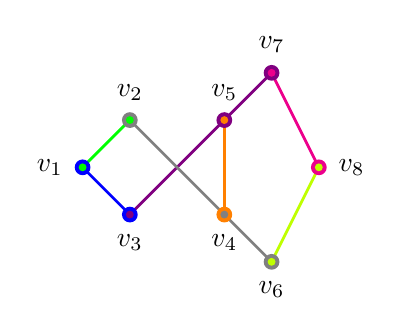
\begin{tikzpicture}  [scale=0.6]
\newdimen\ms
\ms=0.1cm

\tikzstyle{every path}=[line width=1pt]
\tikzstyle{c3}=[circle,inner sep={\ms/8},minimum size=3*\ms]
\tikzstyle{c2}=[circle,inner sep={\ms/8},minimum size=2*\ms]
\tikzstyle{c1}=[circle,inner sep={\ms/8},minimum size=1*\ms]



% Define positions of all observables
\path
  (0,0) coordinate(1)
  (1,1) coordinate(2)
  (1,-1) coordinate(3)
  (3,-1) coordinate(4)
  (3,1) coordinate(5)
  (4,-2) coordinate(6)
  (4,2) coordinate(7)
  (5,0) coordinate(8)
;

% draw contexts

\draw [color=green] (1) -- (2);
\draw [color=blue] (1) -- (3);
\draw [color=violet] (3) --  (5) -- (7);
\draw [color=gray] (2) -- (4) -- (6);
\draw [color=orange] (4) -- (5);
\draw [color=magenta] (7) -- (8);
\draw [color=lime] (6) -- (8);

%
%%
%% draw atoms
%%
%
 \draw (1) coordinate[c2,fill=blue,label=180:$v_1$];
 \draw (1) coordinate[c1,fill=green];
 %
 \draw (2) coordinate[c2,fill=gray,label=90:$v_2$];
 \draw (2) coordinate[c1,fill=green];
 %
 \draw (3) coordinate[c2,fill=blue,label=270:$v_3$];
 \draw (3) coordinate[c1,fill=violet];
 %
 \draw (4) coordinate[c2,fill=orange,label=270:$v_4$];
 \draw (4) coordinate[c1,fill=gray];
 %
 \draw (5) coordinate[c2,fill=violet,label=90:$v_5$];
 \draw (5) coordinate[c1,fill=orange];
 %
 \draw (6) coordinate[c2,fill=gray,label=270:$v_6$];
 \draw (6) coordinate[c1,fill=lime];
 %
 %\draw (7) coordinate[c3,fill=orange];
 \draw (7) coordinate[c2,fill=violet,label=90:$v_7$];
 \draw (7) coordinate[c1,fill=magenta];
 %
 \draw (8) coordinate[c2,fill=magenta,label=0:$v_8$];
 \draw (8) coordinate[c1,fill=lime];

\end{tikzpicture}
&$\,$&
%&&
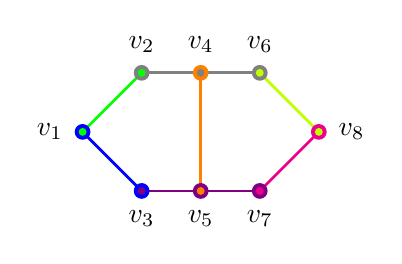
\begin{tikzpicture}  [scale=0.75]
\newdimen\ms
\ms=0.1cm

\tikzstyle{every path}=[line width=1pt]
\tikzstyle{c3}=[circle,inner sep={\ms/8},minimum size=3*\ms]
\tikzstyle{c2}=[circle,inner sep={\ms/8},minimum size=2*\ms]
\tikzstyle{c1}=[circle,inner sep={\ms/8},minimum size=1*\ms]

% Define positions of all observables
\path
  (0,0) coordinate(1)
  (1,1) coordinate(2)
  (1,-1) coordinate(3)
  (2,1) coordinate(4)
  (2,-1) coordinate(5)
  (3,1) coordinate(6)
  (3,-1) coordinate(7)
  (4,0) coordinate(8)
;

% draw contexts

\draw [color=green] (1) -- (2);
\draw [color=blue] (1) -- (3);
\draw [color=violet] (3) --  (5) -- (7);
\draw [color=gray] (2) -- (4) -- (6);
\draw [color=orange] (4) -- (5);
\draw [color=magenta] (7) -- (8);
\draw [color=lime] (6) -- (8);

%
%%
%% draw atoms
%%
%
 \draw (1) coordinate[c2,fill=blue,label=180:$v_1$];
 \draw (1) coordinate[c1,fill=green];
 %
 \draw (2) coordinate[c2,fill=gray,label=90:$v_2$];
 \draw (2) coordinate[c1,fill=green];
 %
 \draw (3) coordinate[c2,fill=blue,label=270:$v_3$];
 \draw (3) coordinate[c1,fill=violet];
 %
 \draw (4) coordinate[c2,fill=orange,label=90:$v_4$];
 \draw (4) coordinate[c1,fill=gray];
 %
 \draw (5) coordinate[c2,fill=violet,label=270:$v_5$];
 \draw (5) coordinate[c1,fill=orange];
 %
 \draw (6) coordinate[c2,fill=gray,label=90:$v_6$];
 \draw (6) coordinate[c1,fill=lime];
 %
 %\draw (7) coordinate[c3,fill=orange];
 \draw (7) coordinate[c2,fill=violet,label=270:$v_7$];
 \draw (7) coordinate[c1,fill=magenta];
 %
 \draw (8) coordinate[c2,fill=magenta,label=0:$v_8$];
 \draw (8) coordinate[c1,fill=lime];

\end{tikzpicture}


\end{tabular}
\end{center}
\caption{\label{Fig3dim}
(Color online)
Two equivalent, isomorphic representations  of the orthogonality diagram of the  the  simplest known~\cite[Fig.~1, p.~182]{kochen2}
TIFS  in $d=3$, with 7 contexts and 8 atomic propositions.
It is realizable in  $S^2$ by taking,
for instance,
$v_1     = (  {0,-1,\sqrt{2}}  )/\sqrt{3}$,
$v_2     = (  {1,0,0}    )$,
$v_3     = (  {1,\sqrt{2},1}   )/ 2 $,
$v_4     = (  {0,1,0}    ) $,
$v_5     = (  {1,0,-1}     )/\sqrt{2}$,
$v_6     = (  {0,0,1}     ) $,
$v_7   = (     {-1,\sqrt{2},-1} )/ 2$,
$v_8   =    ({\sqrt{2},1,0})  / \sqrt{3} $.
Values on $v_1$ and $v_8$ cannot both be 1, as this would imply the values on $v_2=v_3=v_6=v_7=v_9$ to vanish,
which in turn would require both values $v_4$ as well as $v_5$ to be 1; which contradicts exclusivity
because those observables belong to the same context and are orthogonal.
In QT, the proposition $v_i$ is represented by the projector $| v_i \rangle\langle v_i |$.
}
\end{figure}

%%%%%%%%%%%%%%%%%%%%%%%%%%%%%%%%%%%%%%%%%%%%%%%%%%%%%%%%%%%%%%%%%%%

{\em Theorem 1:} Minimal TITS in dimension $d=3$ have 10 vertices.

%%%%%%%%%%%%%%%%%%%%%%%%%%%%%%%%%%%%%%%%%%%%%%%%%%%%%%%%%%%%%%%%%%%

{\em Proof:} This show gets a construction method from the TIFS to obtain a minimal TITS in the same dimension.
It is sufficient to add two vertices, one true vertex $ b $ and other support vertex $ v_3 $ with value no.
Both vertices must belong to $K_d$ by the constraints of the problem, as much as the rest of vertices connected
to $ b $ have value no by TIFS included, simply we must force the value of $ v_3 $ to be no,
which is achieved by simply adding and edge from the true vertex $a$ in the TIFS to vertex $ v_3 $. \endproof

It will be seen later that this method is applicable to higher dimensions.

%%%%%%%%%%%%%%%%%%%%%%%%%%%%%%%%%%%%%%%%%%%%%%%%%%%%%%%%%%%%%%%%%%%

\karl{\bf Do these ar\jr{g}uments also apply for NSS?}
\jr{Not exactly. Searching with 17 vertices is computationally very hard. I am using alternative techniques, but without results (2017-12-02)}

\meil{For $d=3$, Minimum angle = $\arccos(1/3)$ aprox $1.23096$ radian aprox $19.0986º$ (not minutes, decimal point)
Orthonormal representation:
$(0,-1/\sqrt{3},\sqrt{2}/\sqrt{3})$, $(1,0,0)$, $(1/2,1/\sqrt{2},1/2)$, $(0,1,0)$, $(1/\sqrt{2},0,-1/\sqrt{2})$, $(0,0,1)$,
$(-1/2,1/\sqrt{2},-1/2)$, $(\sqrt{2}/\sqrt{3},1/\sqrt{3},0)$.
An orthonormal representation using only 0 and ±1 was done in Pentagrams and Paradoxes and gives the minimal angle too
$(1,1,-1)$, $(0,1,1)$, $(1,0,1)$, $(1,0,0)$, $(0,1,0)$, $(0,1,-1)$, $(1,0,-1)$, $(1,1,1)$.}
%%%%%%%%%%%%%%%%%%%%%%%%%%%%%%%%%%%%%%%%%%%%%%%%%%%%%%%%%%%%%%%%%%%

\jr{\sc The orthogonal representation of the pentagon determines univoquely the orthogonal representation of the entire budge. SEE draft
in actual PAPER SHEET.}

%%%%%%%%%%%%%%%%%%%%%%%%%%%%%%%%%%%%%%%%%%%%%%%%%%%%%%%%%%%%%%%%%%%

\section{Higher dimensions}

\jr{SOME PARAGRAPHS CHANGED ORDER IN THIS SECTION}

%%%%%%%%%%%%%%%%%%%%%%%%%%%%%%%%%%%%%%%%%%%%%%%%%%%%%%%%%%%%%%%%%%%

In this section we generalize the results of the previous section to higher dimensions than 3.

{\em Theorem 2:} Let be $G$ a critical TIFS graph in dimension $d$ with two $K_d$, then $V(G) \geq d+5$.

%%%%%%%%%%%%%%%%%%%%%%%%%%%%%%%%%%%%%%%%%%%%%%%%%%%%%%%%%%%%%%%%%%%

{\em Proof:} For this proof we use the notion of forbidden graph in dimension $d$ for the orthogonal rank of a graph \cite{code21}. This concept is related to the impossible representation of a graph with several structure.

For a non trivial TIFS we have to use a context, so the first valid linked structure in dimension $d$ is $K_{d-1}$ linked to true vertex $y$ and false vertex $x$ such that $N(y) = N(x)$. But this graph ($|V(G)| = d+1$) is not realizable because it form a forbbiden graph in dimension $d$.

Suppose that we have a graph with one more vertex $c$ ($|V(G)| = d+2$). Is evident that $y \nsim c$, so $c$ have to belong to a context with other vertex from $K_{d-1}$ (for now call $Q$). We consider two cases: a) $N(x) = \{v / v \in $Q$\}$, Then we have another forbbiden graph between $c$ and $x$. b) Choose $N(x) \cap N(y) = \emptyset$, in that case we have a forbbiden structure between $y$ and $x$.

We must consider a new vertex $w$ ($|V(G)| = d+3$). Previous results shows that neither $y$ or $x$ can belong to the two $K_d$ necessary for the lemma 5, so the structure between $y$ and $x$ must have two $K_d$, but we only have $c$ and $w$ as internal vertex different of $Q$. Is not enough to evade a forbidden structure again (both will create forbbiden graph).

We introduce another vertex $t$ ($|V(G)| = d+4$). This new vertex will support to anyone internal vertex $w$ or $c$. w.l.o.g. We consider that $t$ support $w$, i.e. They belong to the same context. Now we have two $K_d$ from $c \cup N(c)=Q$ and $w \cup t \cup Q-{q}$ where $q \in N(c)$. Here we can observe that again appear forbbiden structure in dimension $d$ between $t$ and $q$ because $N(t) = N(q)$.

Then we must consider $|V(G)| \geq d+5$ to get a minimal TIFS. In fact, we know a structure of TIFS with $d+5$ vertices
obtained from the Fig.~\ref{Fig3}. \endproof

{\em Example:} The graph $G$ of Fig.~\ref{Fig1}\jr{(a) \sout{,with $V(G) = \{A,v_1,v_2,v_4,v_5,v_6,v_7, v_8\}$,}} is a critical TIFS graph in dimension 3.

\jr{The number of TIFSes in dimension $3,4,5,6...$ is $1,3,4,8,13,19...$
In general, the number of TITFSes in dimension $d$ is $(d^2-d-4)/3$.
We know all the corresponding graphs and its orthogonal representation. In the further sections, we will explain these results.}

{\em Theorem 3:} Let be $G$ a critical TITS that contain a TIFS graph with $d+k$ vertices, then $G$ have, at least, $d+k+2$ vertices.

{\em Proof:} We dismiss two different cases: a) Suppose the critical TITS graph has $d+k$ vertices with yes vertices $a$ and $c$. Then the vertex $c$ must belong to one of two $K_d$ in TIFS with false vertex $b$, in that case reaches vertex $b$ not be affected by the obtained colored TITS with vertices $a$ and $c$ that, for the Lemma 2, contains a smaller TIFS than the original. b) Suppose the critical TITS with $d+k+1$ vertices and true vertex $a, c$. We add a vertex $x$ to TIFS from true vertex $a$ to false vertex $b$, is clear that the new vertex must be yes, i.e., it must be equal to vertex $c$, because if $c$ was an internal vertex of TIFS with $a$ yes and $b$ no then we have the previous case. \endproof

{\em Theorem 4:} Minimal TITS have $d+7$ vertices in dimension $d\geq 3$.

{\em Proof:} The addition of two vertices of the TIFS in dimension $d$ with true vertex $a$ and false vertex $b$ by addition of necessary edges in the TITS with yes vertices $a$ and $c$ can not be a forbidden graph (you can check that the structure with 3 independent triangles full linked to $K_{d-3}$ has dimension $d$), so this obtained a TITS realizable in dimension $d$. The general structure of the graph is in Fig.~\ref{Fig3}. \endproof


%%%%%%%%%%%%%%%%%%%%%%%%%%%%%%%%%%%%%%%%%%%%%%%%%%%%%%%%%%%%%%%%%%%

{\em Corollary 2:} The family of minimal \karl{TITSes} with $d+7$ vertices contains exactly 3 $K_d$.

{\em Proof:} Consider the structure of minimal TITS (Fig.~\ref{Fig3}), where $\{a\} \cup C$ is TIFS in dimension $d$ and $|D| = d-2$. There exist some edges between $C $ \jr{\sout{$\subset TIFS_{d=3}$}} and $D$ that form one more $K_d$. Furthermore, $\forall v \in D$ verifies that $v \in N(a)$. \endproof

%%%%%%%%%%%%%%%%%%%%%%%%%%%%%%%%%%%%%%%%%%%%%%%%%%%%%%%%%%%%%%%%%%%
% Fig. 3
%%%%%%%%%%%%%%%%%%%%%%%%%%%%%%%%%%%%%%%%%%%%%%%%%%%%%%%%%%%%%%%%%%%

\begin{figure}
%\begin{center}
\centering
\centerline{\includegraphics[scale=0.70]{schemaYIYgeneral.pdf}}
%\centerline{\includegraphics[scale=0.70]{Fig3.pdf}}
\caption{\label{Fig3} Schema for minimal TITS with $d+k+2$ vertices in dimension $d$.
The arrow represents connection between $a$ and some vertices in $C$ such that they form a minimal TIFS,
also vertex $a$ is linked with all vertices in $D$.}
%\end{center}
\end{figure}


%%%%%%%%%%%%%%%%%%%%%%%%%%%%%%%%%%%%%%%%%%%%%%%%%%%%%%%%%%%%%%%%%%%

\section{Dimension 4 - Hardy bug \& other bugs}

\jr{There are three TIFS with a minimum number of propositions in dimension $4$\karllate{, as depicted} in Fig~\ref{fig:d4}.}


\jr{TIPS: (a) The orthogonal representation il (almost) unique (b) minimal angle (c) Explain the three graphs}

\meil{For $d=4$, Minimum angle = $\arccos((1-\varepsilon^2)/3)$ por the graphs (a) and (b) in Fig.~\ref{fig:d4} and $\arccos(1/3)$ por graph (c)}

%%%%%%%%%%%%%%%%%%%%%%%%%%%%%%%%%%%%%%%%%%%%%%%%%%%%%%%%%%%%%%%%%%%
% Fig. NN  dim = 4
%%%%%%%%%%%%%%%%%%%%%%%%%%%%%%%%%%%%%%%%%%%%%%%%%%%%%%%%%%%%%%%%%%%
\begin{figure}
\begin{center}
\begin{tabular}{cc}
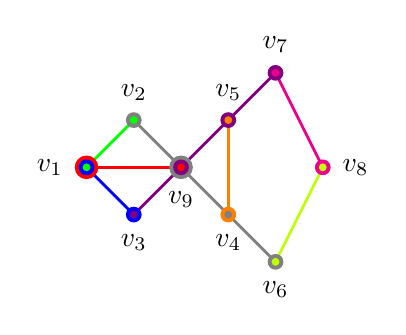
\begin{tikzpicture}  [scale=0.6]
\newdimen\ms
\ms=0.1cm

\tikzstyle{every path}=[line width=1pt]
\tikzstyle{c3}=[circle,inner sep={\ms/8},minimum size=3*\ms]
\tikzstyle{c2}=[circle,inner sep={\ms/8},minimum size=2*\ms]
\tikzstyle{c1}=[circle,inner sep={\ms/8},minimum size=1*\ms]



% Define positions of all observables
\path
  (0,0) coordinate(1)
  (1,1) coordinate(2)
  (1,-1) coordinate(3)
  (3,-1) coordinate(4)
  (3,1) coordinate(5)
  (4,-2) coordinate(6)
  (4,2) coordinate(7)
  (5,0) coordinate(8)
  (2,0) coordinate(9)
;

% draw contexts

\draw [color=green] (1) -- (2);
\draw [color=blue] (1) -- (3);
\draw [color=red] (1) -- (9)  ;
\draw [color=violet] (3) -- (9) -- (5) -- (7);
\draw [color=gray] (2) -- (9) -- (4) -- (6);
\draw [color=orange] (4) -- (5);
\draw [color=magenta] (7) -- (8);
\draw [color=lime] (6) -- (8);

%
%%
%% draw atoms
%%
%
 \draw (1) coordinate[c3,fill=red,label=180:$v_1$];
 \draw (1) coordinate[c2,fill=blue];
 \draw (1) coordinate[c1,fill=green];
 %
 \draw (2) coordinate[c2,fill=gray,label=90:$v_2$];
 \draw (2) coordinate[c1,fill=green];
 %
 \draw (3) coordinate[c2,fill=blue,label=270:$v_3$];
 \draw (3) coordinate[c1,fill=violet];
 %
 \draw (4) coordinate[c2,fill=orange,label=270:$v_4$];
 \draw (4) coordinate[c1,fill=gray];
 %
 \draw (5) coordinate[c2,fill=violet,label=90:$v_5$];
 \draw (5) coordinate[c1,fill=orange];
 %
 \draw (6) coordinate[c2,fill=gray,label=270:$v_6$];
 \draw (6) coordinate[c1,fill=lime];
 %
 %\draw (7) coordinate[c3,fill=orange];
 \draw (7) coordinate[c2,fill=violet,label=90:$v_7$];
 \draw (7) coordinate[c1,fill=magenta];
 %
 \draw (8) coordinate[c2,fill=magenta,label=0:$v_8$];
 \draw (8) coordinate[c1,fill=lime];

 %\draw (8) coordinate[c1,fill=red];
 %
 \draw (9) coordinate[c3,fill=gray,label=270:$v_9$];
 \draw (9) coordinate[c2,fill=violet];
 \draw (9) coordinate[c1,fill=red];

\end{tikzpicture}
%%%%%%%%%%%%%%%%%%%%%%%%%%%%%%%%%%%%%%%%%%%%%%%%%%%%%%%%%%%%%%%%%%%%%%%%%%%%
&
%%%%%%%%%%%%%%%%%%%%%%%%%%%%%%%%%%%%%%%%%%%%%%%%%%%%%%%%%%%%%%%%%%%%%%%%%%%%
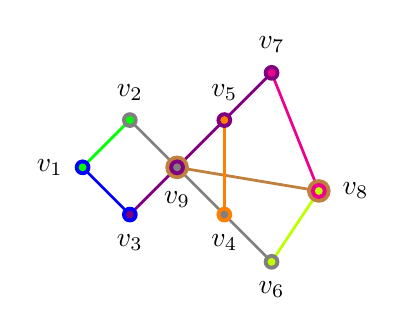
\begin{tikzpicture}  [scale=0.6]
\newdimen\ms
\ms=0.1cm

\tikzstyle{every path}=[line width=1pt]
\tikzstyle{c4}=[circle,inner sep={\ms/8},minimum size=4*\ms]
\tikzstyle{c3}=[circle,inner sep={\ms/8},minimum size=3*\ms]
\tikzstyle{c2}=[circle,inner sep={\ms/8},minimum size=2*\ms]
\tikzstyle{c1}=[circle,inner sep={\ms/8},minimum size=1*\ms]


% Define positions of all observables
\path
  (0,0) coordinate(1)
  (1,1) coordinate(2)
  (1,-1) coordinate(3)
  (3,-1) coordinate(4)
  (3,1) coordinate(5)
  (4,-2) coordinate(6)
  (4,2) coordinate(7)
  (5,-0.5) coordinate(8)
  (2,0) coordinate(9)
;

% draw contexts

\draw [color=green] (1) -- (2);
\draw [color=blue] (1) -- (3);
%\draw [color=red] (1) -- (9) ;
\draw [color=brown] (9) -- (8) ;
\draw [color=violet] (3) -- (9) -- (5) -- (7);
\draw [color=gray] (2) -- (9) -- (4) -- (6);
\draw [color=orange] (4) -- (5);
\draw [color=magenta] (7) -- (8);
\draw [color=lime] (6) -- (8);

%
%%
%% draw atoms
%%
%
 %\draw (1) coordinate[c3,fill=red];
 \draw (1) coordinate[c2,fill=blue,label=180:$v_1$];
 \draw (1) coordinate[c1,fill=green];
 %
 \draw (2) coordinate[c2,fill=gray,label=90:$v_2$];
 \draw (2) coordinate[c1,fill=green];
 %
 \draw (3) coordinate[c2,fill=blue,label=270:$v_3$];
 \draw (3) coordinate[c1,fill=violet];
 %
 \draw (4) coordinate[c2,fill=orange,label=270:$v_4$];
 \draw (4) coordinate[c1,fill=gray];
 %
 \draw (5) coordinate[c2,fill=violet,label=90:$v_5$];
 \draw (5) coordinate[c1,fill=orange];
 %
 \draw (6) coordinate[c2,fill=gray,label=270:$v_6$];
 \draw (6) coordinate[c1,fill=lime];
 %
 %\draw (7) coordinate[c3,fill=orange];
 \draw (7) coordinate[c2,fill=violet,label=90:$v_7$];
 \draw (7) coordinate[c1,fill=magenta];
 %
 \draw (8) coordinate[c3,fill=brown,label=0:$v_8$];
 \draw (8) coordinate[c2,fill=magenta];
 \draw (8) coordinate[c1,fill=lime];

 %\draw (8) coordinate[c1,fill=red];
 %
 \draw (9) coordinate[c3,fill=brown,label=270:$v_9$];
 \draw (9) coordinate[c2,fill=violet];
 \draw (9) coordinate[c1,fill=gray];

\end{tikzpicture}
%%%%%%%%%%%%%%%%%%%%%%%%%%%%%%%%%%%%%%%%%%%%%%%%%%%%%%%%%%%%%%%%%%%%%%%%%%%%
\\ (a)&(b)\\
%%%%%%%%%%%%%%%%%%%%%%%%%%%%%%%%%%%%%%%%%%%%%%%%%%%%%%%%%%%%%%%%%%%%%%%%%%%%
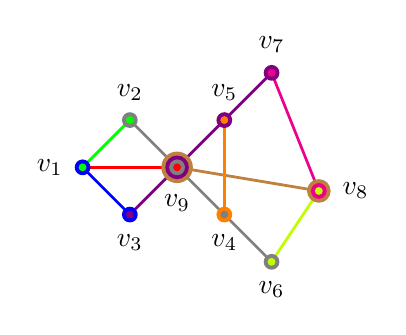
\begin{tikzpicture}  [scale=0.6]
\newdimen\ms
\ms=0.1cm

\tikzstyle{every path}=[line width=1pt]
\tikzstyle{c4}=[circle,inner sep={\ms/8},minimum size=4*\ms]
\tikzstyle{c3}=[circle,inner sep={\ms/8},minimum size=3*\ms]
\tikzstyle{c2}=[circle,inner sep={\ms/8},minimum size=2*\ms]
\tikzstyle{c1}=[circle,inner sep={\ms/8},minimum size=1*\ms]

% Define positions of all observables
\path
  (0,0) coordinate(1)
  (1,1) coordinate(2)
  (1,-1) coordinate(3)
  (3,-1) coordinate(4)
  (3,1) coordinate(5)
  (4,-2) coordinate(6)
  (4,2) coordinate(7)
  (5,-0.5) coordinate(8)
  (2,0) coordinate(9)
;

% draw contexts

\draw [color=green] (1) -- (2);
\draw [color=blue] (1) -- (3);
\draw [color=red] (1) -- (9) ;
\draw [color=brown] (9) -- (8) ;
\draw [color=violet] (3) -- (9) -- (5) -- (7);
\draw [color=gray] (2) -- (9) -- (4) -- (6);
\draw [color=orange] (4) -- (5);
\draw [color=magenta] (7) -- (8);
\draw [color=lime] (6) -- (8);

%
%%
%% draw atoms
%%
%
 %\draw (1) coordinate[c3,fill=red];
 \draw (1) coordinate[c2,fill=blue,label=180:$v_1$];
 \draw (1) coordinate[c1,fill=green];
 %
 \draw (2) coordinate[c2,fill=gray,label=90:$v_2$];
 \draw (2) coordinate[c1,fill=green];
 %
 \draw (3) coordinate[c2,fill=blue,label=270:$v_3$];
 \draw (3) coordinate[c1,fill=violet];
 %
 \draw (4) coordinate[c2,fill=orange,label=270:$v_4$];
 \draw (4) coordinate[c1,fill=gray];
 %
 \draw (5) coordinate[c2,fill=violet,label=90:$v_5$];
 \draw (5) coordinate[c1,fill=orange];
 %
 \draw (6) coordinate[c2,fill=gray,label=270:$v_6$];
 \draw (6) coordinate[c1,fill=lime];
 %
 %\draw (7) coordinate[c3,fill=orange];
 \draw (7) coordinate[c2,fill=violet,label=90:$v_7$];
 \draw (7) coordinate[c1,fill=magenta];
 %
 \draw (8) coordinate[c3,fill=brown,label=0:$v_8$];
 \draw (8) coordinate[c2,fill=magenta];
 \draw (8) coordinate[c1,fill=lime];

 %
  \draw (9) coordinate[c4,fill=brown,label=270:$v_9$];
 \draw (9) coordinate[c3,fill=violet];
 \draw (9) coordinate[c2,fill=gray];
 \draw (9) coordinate[c1,fill=red];

\end{tikzpicture}
\\
 (c)
\end{tabular}
\end{center}
\caption{\label{fig:d4}
(Color online)
Orthogonality diagram of the  the three  simplest (partially known~\cite{Hardy-93,Cab96,Bad11})
TIFS  in $d=4$, with 8(9) contexts and 9 atomic propositions.
It is realizable in  $S^3$ by taking,
for instance,
(a)
$v_1     = (  {0,-1,\sqrt{2},0}  )/\sqrt{3}$,
$v_2     = (  {1,0,0,0}    )$,
$v_3     = (  {1,\sqrt{2},1,0}   )/ 2 $,
$v_4     = (  {0,1,0,0}    ) $,
$v_5     = (  {1,0,-1,0}     )/\sqrt{2}$,
$v_6     = (  {0,0,1,0}     ) $,
$v_7   = (     {-1,\sqrt{2},-1,0} )/ 2$,
$v_8   =      (\sqrt{1-\varepsilon^2} / \sqrt{3})  ({\sqrt{2},1,0,0})+\varepsilon({0,0,0,1})$,
$v_9     = (   {0,0,0,1} )$,
(b)
$v_1     =   (\sqrt{1-\varepsilon^2} / \sqrt{3})(  {0,-1,\sqrt{2},0}  )+\varepsilon({0,0,0,1})$,
$v_8   =  (        {\sqrt{2},1,0,0} )/\sqrt{3}$,
(c)
$v_1     = (  {0,-1,\sqrt{2},0}  )/\sqrt{3}$,
$v_8   =  (        {\sqrt{2},1,0,0} ) /\sqrt{3}$.
Values on $v_1$ and $v_8$ cannot both be 1, as this would imply the values on $v_2=v_3=v_6=v_7=v_9$ to vanish,
which in turn would require both values $v_4$ as well as $v_5$ to be 1; which contradicts exclusivity
because those observables belong to the same context and are orthogonal.
In QT, the proposition $v_i$ is represented by the projector $| v_i \rangle\langle v_i |$.
\jr{FIGURE IN ONE COLUMN.  $\backslash$widetext COMMAND REMOVED}}

\end{figure}

%\clearpage
%\newpage

%\widetext

%%%%%%%%%%%%%%%%%%%%%%%%%%%%%%%%%%%%%%%%%%%%%%%%%%%%%%%%%%%%%%%%%%%%%%%
\subsection{Specific realizations}

\jr{\sc figures to one column, bibtex items to bibtex file CNLG.bib}

\subsubsection{Pentagrams and Paradoxes}
\cite{Bad11}
%\begin{verbatim}
%@article{Bad11,
%doi     = {10.1007/s10701-010-9433-3},
%title   = {Pentagrams and Paradoxes},
%author  = {Piotr Badzi\c{a}g and Ingemar Bengtsson and Ad\'an Cabello and Helena Granstr\"om and Jan-Ake Larsson},
%publisher       = {Springer US},
%journal = {Foundations of Physics},
%issnp   = {0015-9018},
%issne   = {1572-9516},
%year    = {2011},
%month   = {03},
%volume  = {41},
%issue   = {3},
%page    = {414-423},
%url =       {http://doi.org/10.1007/s10701-010-9433-3},
%}
%\end{verbatim}



\begin{figure}
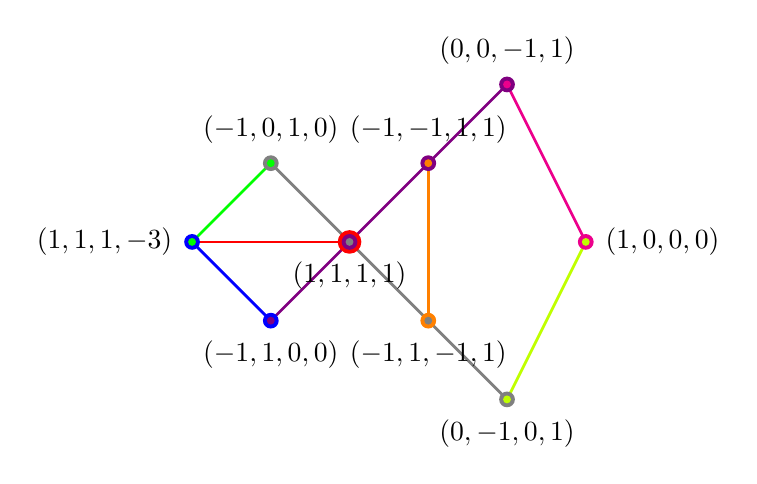
\begin{tikzpicture}  [scale=1]
\newdimen\ms
\ms=0.1cm

\tikzstyle{every path}=[line width=1pt]
\tikzstyle{c3}=[circle,inner sep={\ms/8},minimum size=3*\ms]
\tikzstyle{c2}=[circle,inner sep={\ms/8},minimum size=2*\ms]
\tikzstyle{c1}=[circle,inner sep={\ms/8},minimum size=1*\ms]

% Radius of regular polygons
\newdimen\R
\R=5cm
%\r= { \R * sqrt(3)/2}
\newdimen\S
\S=2.5cm

% Define positions of all observables
\path
  (0,0) coordinate(1)
  (1,1) coordinate(2)
  (1,-1) coordinate(3)
  (3,-1) coordinate(4)
  (3,1) coordinate(5)
  (4,-2) coordinate(6)
  (4,2) coordinate(7)
  (5,0) coordinate(8)
  (2,0) coordinate(9)
;

% draw contexts

\draw [color=green] (1) -- (2);
\draw [color=blue] (1) -- (3);
\draw [color=red] (1) -- (9)  ;
\draw [color=violet] (3) -- (9) -- (5) -- (7);
\draw [color=gray] (2) -- (9) -- (4) -- (6);
\draw [color=orange] (4) -- (5);
\draw [color=magenta] (7) -- (8);
\draw [color=lime] (6) -- (8);

%
%%
%% draw atoms
%%
%
  %\draw (1) coordinate[c3,fill=red];
 \draw (1) coordinate[c2,fill=blue,label=180:{$(1,1,1,-3)$}];
 \draw (1) coordinate[c1,fill=green];
 %
  \draw (2) coordinate[c2,fill=gray,label=90:{$(-1,0,1,0  )$}];
 \draw (2) coordinate[c1,fill=green];
 %
 \draw (3) coordinate[c2,fill=blue,label=270:{$(-1,1,0,0  )$}];
 \draw (3) coordinate[c1,fill=violet];
 %
 \draw (4) coordinate[c2,fill=orange,label=270:{$(-1,1,-1,1 )$}];
 \draw (4) coordinate[c1,fill=gray];
 %
 \draw (5) coordinate[c2,fill=violet,label=90:{$(-1,-1,1,1 )$}];
 \draw (5) coordinate[c1,fill=orange];
 %
 \draw (6) coordinate[c2,fill=gray,label=270:{$(0,-1,0,1  )$}];
 \draw (6) coordinate[c1,fill=lime];
 %
 %\draw (7) coordinate[c3,fill=orange];
 \draw (7) coordinate[c2,fill=violet,label=90:{$(0,0,-1,1  )$}];
 \draw (7) coordinate[c1,fill=magenta];
 %
 %\draw (8) coordinate[c3,fill=brown];
 \draw (8) coordinate[c2,fill=magenta,label=0:{$(1,0,0,0   )$}];
 \draw (8) coordinate[c1,fill=lime];

 %\draw (8) coordinate[c1,fill=red];
 %
 \draw (9) coordinate[c3,fill=red];
 \draw (9) coordinate[c2,fill=violet,label=270:{$(1,1,1,1)$}];
 \draw (9) coordinate[c1,fill=gray];
%\draw (14) coordinate[c1,fill=cyan];

\end{tikzpicture}
\caption{Pentagrams and Paradoxes\cite{Bad11}}
\end{figure}

%\clearpage
%\newpage

\subsubsection{No-hidden-variables proof for two spin-particles preselected and postselected in unentangled states}
%\begin{verbatim}
%@article{Cab97,
%  title = {No-hidden-variables proof for two spin- particles preselected and postselected in unentangled states},
%  author = {Cabello, Ad\'an},
%  journal = {Physical Review A},
%  volume = {55},
%  issue = {6},
%  pages = {4109-4111},
%  numpages = {0},
%  year = {1997},
%  month = {Jun},
%  publisher = {American Physical Society},
%  doi = {10.1103/PhysRevA.55.4109},
%  url = {http://doi.org/doi/10.1103/PhysRevA.55.4109}
%}
%\end{verbatim}

\cite{Cab97}

\begin{figure}
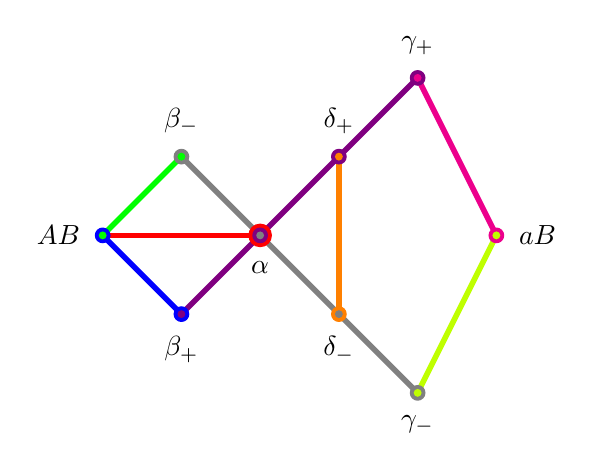
\begin{tikzpicture}  [scale=1]
\newdimen\ms
\ms=0.1cm

\tikzstyle{every path}=[line width=2pt]
\tikzstyle{c3}=[circle,inner sep={\ms/8},minimum size=3*\ms]
\tikzstyle{c2}=[circle,inner sep={\ms/8},minimum size=2*\ms]
\tikzstyle{c1}=[circle,inner sep={\ms/8},minimum size=1*\ms]

% Radius of regular polygons
\newdimen\R
\R=5cm
%\r= { \R * sqrt(3)/2}
\newdimen\S
\S=2.5cm

% Define positions of all observables
\path
  (0,0) coordinate(1)
  (1,1) coordinate(2)
  (1,-1) coordinate(3)
  (3,-1) coordinate(4)
  (3,1) coordinate(5)
  (4,-2) coordinate(6)
  (4,2) coordinate(7)
  (5,0) coordinate(8)
  (2,0) coordinate(9)
;

% draw contexts

\draw [color=green] (1) -- (2);
\draw [color=blue] (1) -- (3);
\draw [color=red] (1) -- (9)  ;
\draw [color=violet] (3) -- (9) -- (5) -- (7);
\draw [color=gray] (2) -- (9) -- (4) -- (6);
\draw [color=orange] (4) -- (5);
\draw [color=magenta] (7) -- (8);
\draw [color=lime] (6) -- (8);

%
%%
%% draw atoms
%%
%
  %\draw (1) coordinate[c3,fill=red];
 \draw (1) coordinate[c2,fill=blue,label=180:{$AB$}];
 \draw (1) coordinate[c1,fill=green];
 %
  \draw (2) coordinate[c2,fill=gray,label=90:{$\beta_-$}];
 \draw (2) coordinate[c1,fill=green];
 %
 \draw (3) coordinate[c2,fill=blue,label=270:{$\beta_+$}];
 \draw (3) coordinate[c1,fill=violet];
 %
 \draw (4) coordinate[c2,fill=orange,label=270:{$\delta_-$}];
 \draw (4) coordinate[c1,fill=gray];
 %
 \draw (5) coordinate[c2,fill=violet,label=90:{$\delta_+$}];
 \draw (5) coordinate[c1,fill=orange];
 %
 \draw (6) coordinate[c2,fill=gray,label=270:{$\gamma_-$}];
 \draw (6) coordinate[c1,fill=lime];
 %
 %\draw (7) coordinate[c3,fill=orange];
 \draw (7) coordinate[c2,fill=violet,label=90:{$\gamma_+$}];
 \draw (7) coordinate[c1,fill=magenta];
 %
 %\draw (8) coordinate[c3,fill=brown];
 \draw (8) coordinate[c2,fill=magenta,label=0:{$aB$}];
 \draw (8) coordinate[c1,fill=lime];

 %\draw (8) coordinate[c1,fill=red];
 %
 \draw (9) coordinate[c3,fill=red,label=270:{$\alpha$}];
 \draw (9) coordinate[c2,fill=violet];
 \draw (9) coordinate[c1,fill=gray];
%%
%\draw (10) coordinate[c2,fill=blue];
%\draw (10) coordinate[c1,fill=blue];
%%
%\draw (11) coordinate[c2,fill=blue];
%\draw (11) coordinate[c1,fill=red];
%%
%\draw (12) coordinate[c1,fill=red];
%%
%\draw (13) coordinate[c1,fill=lime];
%%
%\draw (14) coordinate[c2,fill=orange,label=0:$\quad 7$];
%\draw (14) coordinate[c1,fill=cyan];

\end{tikzpicture}
\\
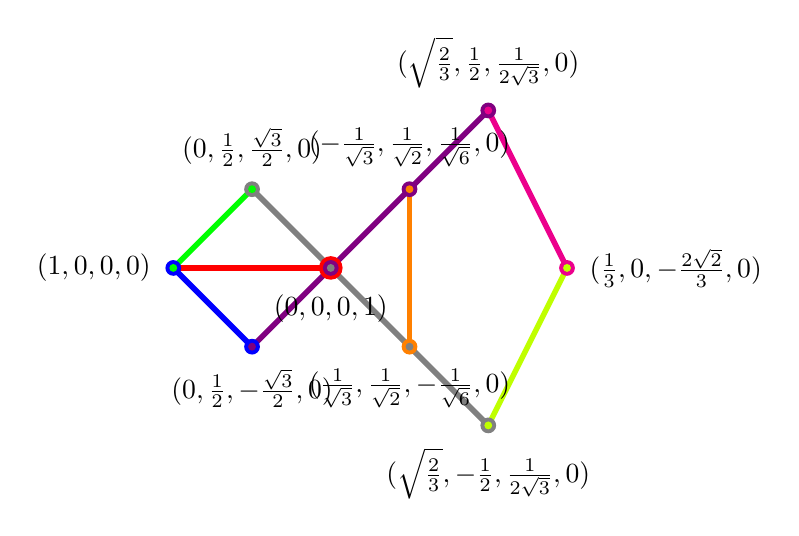
\begin{tikzpicture}  [scale=1]
\newdimen\ms
\ms=0.1cm

\tikzstyle{every path}=[line width=2pt]
\tikzstyle{c3}=[circle,inner sep={\ms/8},minimum size=3*\ms]
\tikzstyle{c2}=[circle,inner sep={\ms/8},minimum size=2*\ms]
\tikzstyle{c1}=[circle,inner sep={\ms/8},minimum size=1*\ms]

% Radius of regular polygons
\newdimen\R
\R=5cm
%\r= { \R * sqrt(3)/2}
\newdimen\S
\S=2.5cm

% Define positions of all observables
\path
  (0,0) coordinate(1)
  (1,1) coordinate(2)
  (1,-1) coordinate(3)
  (3,-1) coordinate(4)
  (3,1) coordinate(5)
  (4,-2) coordinate(6)
  (4,2) coordinate(7)
  (5,0) coordinate(8)
  (2,0) coordinate(9)
;

% draw contexts

\draw [color=green] (1) -- (2);
\draw [color=blue] (1) -- (3);
\draw [color=red] (1) -- (9)  ;
\draw [color=violet] (3) -- (9) -- (5) -- (7);
\draw [color=gray] (2) -- (9) -- (4) -- (6);
\draw [color=orange] (4) -- (5);
\draw [color=magenta] (7) -- (8);
\draw [color=lime] (6) -- (8);

%
%%
%% draw atoms
%%
%
  %\draw (1) coordinate[c3,fill=red];
 \draw (1) coordinate[c2,fill=blue,label=180:{$(1 , 0 , 0 , 0)$}];
 \draw (1) coordinate[c1,fill=green];
 %
  \draw (2) coordinate[c2,fill=gray,label=90:{$(0 , \frac{1}{2} , \frac{\sqrt{3}}{2} , 0 )$}];
 \draw (2) coordinate[c1,fill=green];
 %
 \draw (3) coordinate[c2,fill=blue,label=270:{$(0 , \frac{1}{2} , -\frac{\sqrt{3}}{2} , 0 )$}];
 \draw (3) coordinate[c1,fill=violet];
 %
 \draw (4) coordinate[c2,fill=orange,label=270:{$(\frac{1}{\sqrt{3}} , \frac{1}{\sqrt{2}} ,-\frac{1}{\sqrt{6}} , 0)$}];
 \draw (4) coordinate[c1,fill=gray];
 %
 \draw (5) coordinate[c2,fill=violet,label=90:{$(-\frac{1}{\sqrt{3}} , \frac{1}{\sqrt{2}} , \frac{1}{\sqrt{6}} , 0 )$}];
 \draw (5) coordinate[c1,fill=orange];
 %
 \draw (6) coordinate[c2,fill=gray,label=270:{$( \sqrt{\frac{2}{3}} , -\frac{1}{2} , \frac{1}{2 \sqrt{3}} , 0 )$}];
 \draw (6) coordinate[c1,fill=lime];
 %
 %\draw (7) coordinate[c3,fill=orange];
 \draw (7) coordinate[c2,fill=violet,label=90:{$(\sqrt{\frac{2}{3}} , \frac{1}{2} , \frac{1}{2 \sqrt{3}} , 0 )$}];
 \draw (7) coordinate[c1,fill=magenta];
 %
 %\draw (8) coordinate[c3,fill=red];
 \draw (8) coordinate[c2,fill=magenta,label=0:{$ (\frac{1}{3} , 0 , -\frac{2 \sqrt{2}}{3} , 0 )$}];
 \draw (8) coordinate[c1,fill=lime];

 %\draw (8) coordinate[c1,fill=red];
 %
 \draw (9) coordinate[c3,fill=red,label=270:{$(0 , 0 , 0 , 1 )$}];
 \draw (9) coordinate[c2,fill=violet];
 \draw (9) coordinate[c1,fill=gray];
%%
%\draw (10) coordinate[c2,fill=blue];
%\draw (10) coordinate[c1,fill=blue];
%%
%\draw (11) coordinate[c2,fill=blue];
%\draw (11) coordinate[c1,fill=red];
%%
%\draw (12) coordinate[c1,fill=red];
%%
%\draw (13) coordinate[c1,fill=lime];
%%
%\draw (14) coordinate[c2,fill=orange,label=0:$\quad 7$];
%\draw (14) coordinate[c1,fill=cyan];

\end{tikzpicture}
\caption{No-hidden-variables proof for two spin-particles preselected and postselected in unentangled states~\cite{Cab97}}
\end{figure}

%\clearpage
%\newpage

\subsubsection{{B}ell-{K}ochen-{S}pecker theorem: A proof with 18 vectors}
\jr{\cite{Cab96}}

\jr{MAYBE A FIGURE WITH CABELLO18 GRAPH AND THE BUGDET INSIDE?}


%\begin{verbatim}
%@Article{Cab96,
%  Title                    = {{B}ell-{K}ochen-{S}pecker theorem: A proof with 18 vectors},
%  Author                   = {Ad{\'{a}}n Cabello and Jos{\'{e}} M. Estebaranz and G. Garc{\'{i}}a-Alcaine},
%  Journal                  = {Physics Letters A},
%  Year                     = {1996},
%  Number                   = {4},
%  Pages                    = {183-187},
%  Volume                   = {212},
%  eprint={arXiv:quant-ph/9706009},
%
%  Doi                      = {10.1016/0375-9601(96)00134-X},
%  Url                      = {http://doi.org/10.1016/0375-9601(96)00134-X}
%}
%\end{verbatim}


\begin{figure}
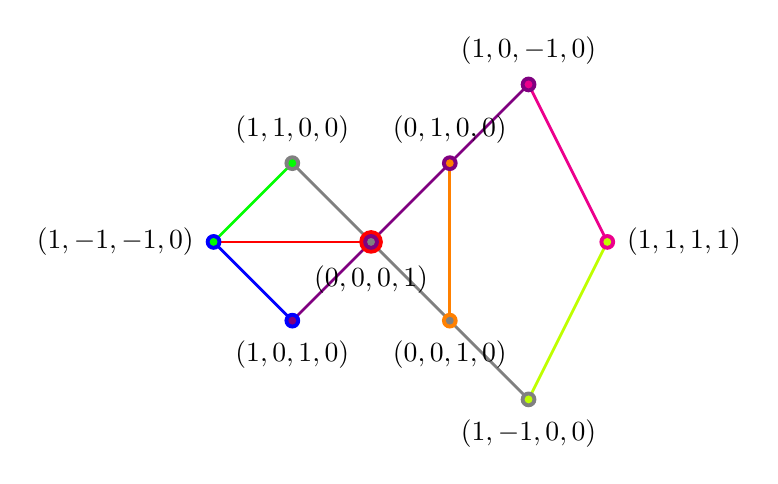
\begin{tikzpicture}  [scale=1]
\newdimen\ms
\ms=0.1cm

\tikzstyle{every path}=[line width=1pt]
\tikzstyle{c3}=[circle,inner sep={\ms/8},minimum size=3*\ms]
\tikzstyle{c2}=[circle,inner sep={\ms/8},minimum size=2*\ms]
\tikzstyle{c1}=[circle,inner sep={\ms/8},minimum size=1*\ms]

% Radius of regular polygons
\newdimen\R
\R=5cm
%\r= { \R * sqrt(3)/2}
\newdimen\S
\S=2.5cm

% Define positions of all observables
\path
  (0,0) coordinate(1)
  (1,1) coordinate(2)
  (1,-1) coordinate(3)
  (3,-1) coordinate(4)
  (3,1) coordinate(5)
  (4,-2) coordinate(6)
  (4,2) coordinate(7)
  (5,0) coordinate(8)
  (2,0) coordinate(9)
;

% draw contexts

\draw [color=green] (1) -- (2);
\draw [color=blue] (1) -- (3);
\draw [color=red] (1) -- (9)  ;
\draw [color=violet] (3) -- (9) -- (5) -- (7);
\draw [color=gray] (2) -- (9) -- (4) -- (6);
\draw [color=orange] (4) -- (5);
\draw [color=magenta] (7) -- (8);
\draw [color=lime] (6) -- (8);

%
%%
%% draw atoms
%%
%
  %\draw (1) coordinate[c3,fill=red];
 \draw (1) coordinate[c2,fill=blue,label=180:{$(1,-1,-1,0)$}];
 \draw (1) coordinate[c1,fill=green];
 %
  \draw (2) coordinate[c2,fill=gray,label=90:{$(1,1,0,0  )$}];
 \draw (2) coordinate[c1,fill=green];
 %
 \draw (3) coordinate[c2,fill=blue,label=270:{$(1,0,1,0  )$}];
 \draw (3) coordinate[c1,fill=violet];
 %
 \draw (4) coordinate[c2,fill=orange,label=270:{$(0,0,1,0 )$}];
 \draw (4) coordinate[c1,fill=gray];
 %
 \draw (5) coordinate[c2,fill=violet,label=90:{$(0,1,0,0 )$}];
 \draw (5) coordinate[c1,fill=orange];
 %
 \draw (6) coordinate[c2,fill=gray,label=270:{$(1,-1,0,0)$}];
 \draw (6) coordinate[c1,fill=lime];
 %
 %\draw (7) coordinate[c3,fill=orange];
 \draw (7) coordinate[c2,fill=violet,label=90:{$(1 , 0,-1,0)$}];
 \draw (7) coordinate[c1,fill=magenta];
 %
 %\draw (8) coordinate[c3,fill=brown];
 \draw (8) coordinate[c2,fill=magenta,label=0:{$(1,1,1,1)$}];
 \draw (8) coordinate[c1,fill=lime];

 %\draw (8) coordinate[c1,fill=red];
 %
 \draw (9) coordinate[c3,fill=red,label=270:{$(0,0,0,1)$}];
 \draw (9) coordinate[c2,fill=violet];
 \draw (9) coordinate[c1,fill=gray];
%%

\end{tikzpicture}
\caption{{B}ell-{K}ochen-{S}pecker theorem: A proof with 18 vectors~\cite{Cab96}}
\end{figure}

%\clearpage
%\newpage


\section{Dimension 5 - generalized Hardy bugs}

\jr{There are four TIFS with a minimum number of propositions in dimension $5$. They are shown in Fig~\ref{fig:d5}.}

\jr{TIPS: (a) The orthogonal representation il (almost) unique (b) Explain the four graphs}

\meil{For $d=5$, Minimum angle = $\arccos((1-\varepsilon^2)/3)$ for all graphs (a) and (b) in Fig.~\ref{fig:d4} except $\arccos(1/3)$ por graph (d)}
%\jr{REVIEWING THIS 2017-01-15}

%%%%%%%%%%%%%%%%%%%%%%%%%%%%%%%%%%%%%%%%%%%%%%%%%%%%%%%%%%%%%%%%%%%
% Fig. NN dim5
%%%%%%%%%%%%%%%%%%%%%%%%%%%%%%%%%%%%%%%%%%%%%%%%%%%%%%%%%%%%%%%%%%%
\begin{figure*}
\begin{center}
\begin{tabular}{cc}
%%%%%%%%%%%%%%%%%%%%%%%%%%%%%%%%%%%%%%%%%%%%%%%%%%%%%%%%%%%%%%%%%%%%%%%%%%%%
%%%%%%%%%%%%%%%%%%%%%%%%%%%%%%%%%%%%%%%%%%%%%%%%%%%%%%%%%%%%%%%%%%%%%%%%%%%
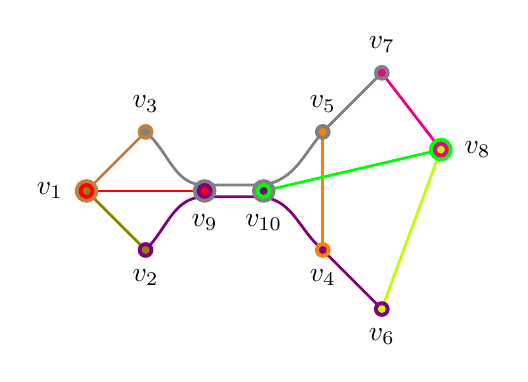
\begin{tikzpicture}  [scale=0.75]
\newdimen\ms
\ms=0.1cm

\tikzstyle{every path}=[line width=1pt]
\tikzstyle{c4}=[circle,inner sep={\ms/8},minimum size=4*\ms]
\tikzstyle{c3}=[circle,inner sep={\ms/8},minimum size=3*\ms]
\tikzstyle{c2}=[circle,inner sep={\ms/8},minimum size=2*\ms]
\tikzstyle{c1}=[circle,inner sep={\ms/8},minimum size=1*\ms]

% Radius of regular polygons
\newdimen\R
\R=5cm
%\r= { \R * sqrt(3)/2}
\newdimen\S
\S=2.5cm

% Define positions of all observables
\path
  (0,0) coordinate(1)
  (1,1) coordinate(3)
  (1,-1) coordinate(2)
  (4,-1) coordinate(4)
  (4,1) coordinate(5)
  (5,-2) coordinate(6)
  (5,2) coordinate(7)
  (6,0.7) coordinate(8)
  (2,0) coordinate(9)
  (3,0) coordinate(10)
  (3,0.1) coordinate(11)
  (2,0.1) coordinate(12)
  (3,-0.1) coordinate(13)
  (2,-0.1) coordinate(14)
;

% draw contexts

\draw [color=olive] (1) -- (2);
\draw [color=brown] (1) -- (3);
\draw [color=violet] (2)  to   [out=45,in=180] (14) -- (13) to [out=-10,in=140] (4) -- (6);
\draw [color=gray] (3)  to [out=320,in=180]  (12) -- (11)  to [out= 10,in=230]  (5) -- (7);
\draw [color=orange] (4) -- (5);
\draw [color=magenta] (7) -- (8);
\draw [color=lime] (6) -- (8);
\draw [color=red]  (9) -- (1);
\draw [color=green] (10) -- (8);
%\draw [color=green] (9) -- (8);

%
%%
%% draw atoms
%%
%
 \draw (1) coordinate[c3,fill=brown,label=180:$v_1$];
 \draw (1) coordinate[c2,fill=red];
 \draw (1) coordinate[c1,fill=olive];
 %
 \draw (2) coordinate[c2,fill=violet,label=270:$v_2$];
 \draw (2) coordinate[c1,fill=olive];
 %
 \draw (3) coordinate[c2,fill=brown,label=90:$v_3$];
 \draw (3) coordinate[c1,fill=gray];
 %
 \draw (4) coordinate[c2,fill=orange,label=270:$v_4$];
 \draw (4) coordinate[c1,fill=violet];
 %
 \draw (5) coordinate[c2,fill=gray,label=90:$v_5$];
 \draw (5) coordinate[c1,fill=orange];
 %
 \draw (6) coordinate[c2,fill=violet,label=270:$v_6$];
 \draw (6) coordinate[c1,fill=lime];
 %
 %\draw (7) coordinate[c3,fill=orange];
 \draw (7) coordinate[c2,fill=gray,label=90:$v_7$];
 \draw (7) coordinate[c1,fill=magenta];
 %
 \draw (8) coordinate[c3,fill=green,label=0:$v_8$];
 \draw (8) coordinate[c2,fill=magenta];
 \draw (8) coordinate[c1,fill=lime];

 %\draw (8) coordinate[c1,fill=red];
 %



  \draw (9) coordinate[c3,fill=gray,label=270:$v_9$];
 \draw (9) coordinate[c2,fill=violet];
 \draw (9) coordinate[c1,fill=red];

  \draw (10) coordinate[c3,fill=gray,label=270:$v_{10}$];
 % \draw (10) coordinate[c3,fill=red];
  \draw (10) coordinate[c2,fill=green];
 \draw (10) coordinate[c1,fill=violet];
%%
%\draw (10) coordinate[c2,fill=brown];
%\draw (10) coordinate[c1,fill=brown];
%%
%\draw (11) coordinate[c2,fill=brown];
%\draw (11) coordinate[c1,fill=red];
%%
%\draw (12) coordinate[c1,fill=red];
%%
%\draw (13) coordinate[c1,fill=lime];
%%
%\draw (14) coordinate[c2,fill=orange,label=0:$\quad 7$];
%\draw (14) coordinate[c1,fill=cyan];

\end{tikzpicture}
%%%%%%%%%%%%%%%%%%%%%%%%%%%%%%%%%%%%%%%%%%%%%%%%%%%%%%%%%%%%%%%%%%%%%%%%%%%%
%\\  (a) \\
&
%%%%%%%%%%%%%%%%%%%%%%%%%%%%%%%%%%%%%%%%%%%%%%%%%%%%%%%%%%%%%%%%%%%%%%%%%%%%%%%%%%%%%%%%%%%%%%%%%%%%%%%%%%%%%%%%%%%%%%%%%%%%%%%%%%%%%%%%%%%%%%%%%%%%%%%%
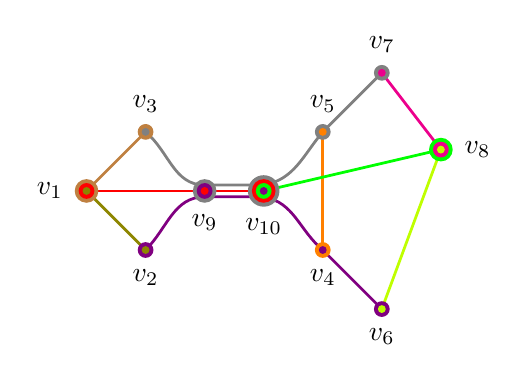
\begin{tikzpicture}  [scale=0.75]
\newdimen\ms
\ms=0.1cm

\tikzstyle{every path}=[line width=1pt]
\tikzstyle{c4}=[circle,inner sep={\ms/8},minimum size=4*\ms]
\tikzstyle{c3}=[circle,inner sep={\ms/8},minimum size=3*\ms]
\tikzstyle{c2}=[circle,inner sep={\ms/8},minimum size=2*\ms]
\tikzstyle{c1}=[circle,inner sep={\ms/8},minimum size=1*\ms]

% Radius of regular polygons
\newdimen\R
\R=5cm
%\r= { \R * sqrt(3)/2}
\newdimen\S
\S=2.5cm

% Define positions of all observables
\path
  (0,0) coordinate(1)
  (1,1) coordinate(3)
  (1,-1) coordinate(2)
  (4,-1) coordinate(4)
  (4,1) coordinate(5)
  (5,-2) coordinate(6)
  (5,2) coordinate(7)
  (6,0.7) coordinate(8)
  (2,0) coordinate(9)
  (3,0) coordinate(10)
  (3,0.1) coordinate(11)
  (2,0.1) coordinate(12)
  (3,-0.1) coordinate(13)
  (2,-0.1) coordinate(14)
;

% draw contexts

\draw [color=olive] (1) -- (2);
\draw [color=brown] (1) -- (3);
\draw [color=violet] (2)  to   [out=45,in=180] (14) -- (13) to [out=-10,in=140] (4) -- (6);
\draw [color=gray] (3)  to [out=320,in=180]  (12) -- (11)  to [out= 10,in=230]  (5) -- (7);
\draw [color=orange] (4) -- (5);
\draw [color=magenta] (7) -- (8);
\draw [color=lime] (6) -- (8);
\draw [color=red] (10) -- (9) -- (1);
\draw [color=green] (10) -- (8);
%\draw [color=green] (9) -- (8);

%
%%
%% draw atoms
%%
%
 \draw (1) coordinate[c3,fill=brown,label=180:$v_1$];
 \draw (1) coordinate[c2,fill=red];
 \draw (1) coordinate[c1,fill=olive];
 %
 \draw (2) coordinate[c2,fill=violet,label=270:$v_2$];
 \draw (2) coordinate[c1,fill=olive];
 %
 \draw (3) coordinate[c2,fill=brown,label=90:$v_3$];
 \draw (3) coordinate[c1,fill=gray];
 %
 \draw (4) coordinate[c2,fill=orange,label=270:$v_4$];
 \draw (4) coordinate[c1,fill=violet];
 %
 \draw (5) coordinate[c2,fill=gray,label=90:$v_5$];
 \draw (5) coordinate[c1,fill=orange];
 %
 \draw (6) coordinate[c2,fill=violet,label=270:$v_6$];
 \draw (6) coordinate[c1,fill=lime];
 %
 %\draw (7) coordinate[c3,fill=orange];
 \draw (7) coordinate[c2,fill=gray,label=90:$v_7$];
 \draw (7) coordinate[c1,fill=magenta];
 %
 \draw (8) coordinate[c3,fill=green,label=0:$v_8$];
 \draw (8) coordinate[c2,fill=magenta];
 \draw (8) coordinate[c1,fill=lime];

 %\draw (8) coordinate[c1,fill=red];
 %



  \draw (9) coordinate[c3,fill=gray,label=270:$v_9$];
 \draw (9) coordinate[c2,fill=violet];
 \draw (9) coordinate[c1,fill=red];

  \draw (10) coordinate[c4,fill=gray,label=270:$v_{10}$];
  \draw (10) coordinate[c3,fill=red];
  \draw (10) coordinate[c2,fill=green];
 \draw (10) coordinate[c1,fill=violet];
%%
%\draw (10) coordinate[c2,fill=brown];
%\draw (10) coordinate[c1,fill=brown];
%%
%\draw (11) coordinate[c2,fill=brown];
%\draw (11) coordinate[c1,fill=red];
%%
%\draw (12) coordinate[c1,fill=red];
%%
%\draw (13) coordinate[c1,fill=lime];
%%
%\draw (14) coordinate[c2,fill=orange,label=0:$\quad 7$];
%\draw (14) coordinate[c1,fill=cyan];

\end{tikzpicture}
%%%%%%%%%%%%%%%%%%%%%%%%%%%%%%%%%%%%%%%%%%%%%%%%%%%%%%%%%%%%%%%%%%%%%%%%%%%%
\\ (a) &  (b) \\
%%%%%%%%%%%%%%%%%%%%%%%%%%%%%%%%%%%%%%%%%%%%%%%%%%%%%%%%%%%%%%%%%%%%%%%%%%%%%%%%%%%%%%%%%%%%%%%%%%%%%%%%%%%%%%%%%%%%%%%%%%%%%%%%%%%%%%%%%%%%%%%%%%%%%%%%
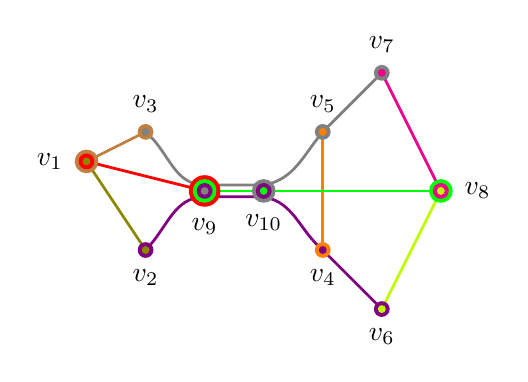
\begin{tikzpicture}  [scale=0.75]
\newdimen\ms
\ms=0.1cm

\tikzstyle{every path}=[line width=1pt]
\tikzstyle{c4}=[circle,inner sep={\ms/8},minimum size=4*\ms]
\tikzstyle{c3}=[circle,inner sep={\ms/8},minimum size=3*\ms]
\tikzstyle{c2}=[circle,inner sep={\ms/8},minimum size=2*\ms]
\tikzstyle{c1}=[circle,inner sep={\ms/8},minimum size=1*\ms]

% Radius of regular polygons
\newdimen\R
\R=5cm
%\r= { \R * sqrt(3)/2}
\newdimen\S
\S=2.5cm

% Define positions of all observables
\path
  (0,0.5) coordinate(1)
  (1,1) coordinate(3)
  (1,-1) coordinate(2)
  (4,-1) coordinate(4)
  (4,1) coordinate(5)
  (5,-2) coordinate(6)
  (5,2) coordinate(7)
  (6,0) coordinate(8)
  (2,0) coordinate(9)
  (3,0) coordinate(10)
  (3,0.1) coordinate(11)
  (2,0.1) coordinate(12)
  (3,-0.1) coordinate(13)
  (2,-0.1) coordinate(14)
;

% draw contexts

\draw [color=olive] (1) -- (2);
\draw [color=brown] (1) -- (3);
\draw [color=violet] (2)  to   [out=45,in=180] (14) -- (13) to [out=-10,in=140] (4) -- (6);
\draw [color=gray] (3)  to [out=320,in=180]  (12) -- (11)  to [out= 10,in=230]  (5) -- (7);
\draw [color=orange] (4) -- (5);
\draw [color=magenta] (7) -- (8);
\draw [color=lime] (6) -- (8);
\draw [color=red] (1) -- (9)  ;
\draw [color=green] (9) -- (10) -- (8);
%
%%
%% draw atoms
%%
%
 \draw (1) coordinate[c3,fill=brown,label=180:$v_1$];
 \draw (1) coordinate[c2,fill=red];
 \draw (1) coordinate[c1,fill=olive];
 %
 \draw (2) coordinate[c2,fill=violet,label=270:$v_2$];
 \draw (2) coordinate[c1,fill=olive];
 %
 \draw (3) coordinate[c2,fill=brown,label=90:$v_3$];
 \draw (3) coordinate[c1,fill=gray];
 %
 \draw (4) coordinate[c2,fill=orange,label=270:$v_4$];
 \draw (4) coordinate[c1,fill=violet];
 %
 \draw (5) coordinate[c2,fill=gray,label=90:$v_5$];
 \draw (5) coordinate[c1,fill=orange];
 %
 \draw (6) coordinate[c2,fill=violet,label=270:$v_6$];
 \draw (6) coordinate[c1,fill=lime];
 %
 %\draw (7) coordinate[c3,fill=orange];
 \draw (7) coordinate[c2,fill=gray,label=90:$v_7$];
 \draw (7) coordinate[c1,fill=magenta];
 %
\draw (8) coordinate[c3,fill=green,label=0:$v_8$];
 \draw (8) coordinate[c2,fill=magenta];
 \draw (8) coordinate[c1,fill=lime];

 %\draw (8) coordinate[c1,fill=red];
 %

 \draw (9) coordinate[c4,fill=red,label=270:$v_9$];
   \draw (9) coordinate[c3,fill=green];
 \draw (9) coordinate[c2,fill=violet];
 \draw (9) coordinate[c1,fill=gray];

  \draw (10) coordinate[c3,fill=gray,label=270:$v_{10}$];
 \draw (10) coordinate[c2,fill=violet];
 \draw (10) coordinate[c1,fill=green];


%%
%\draw (10) coordinate[c2,fill=brown];
%\draw (10) coordinate[c1,fill=brown];
%%
%\draw (11) coordinate[c2,fill=brown];
%\draw (11) coordinate[c1,fill=red];
%%
%\draw (12) coordinate[c1,fill=red];
%%
%\draw (13) coordinate[c1,fill=lime];
%%
%\draw (14) coordinate[c2,fill=orange,label=0:$\quad 7$];
%\draw (14) coordinate[c1,fill=cyan];

\end{tikzpicture}
%%%%%%%%%%%%%%%%%%%%%%%%%%%%%%%%%%%%%%%%%%%%%%%%%%%%%%%%%%%%%%%%%%%%%%%%%%%%
%\\  (c) \\
&
%%%%%%%%%%%%%%%%%%%%%%%%%%%%%%%%%%%%%%%%%%%%%%%%%%%%%%%%%%%%%%%%%%%%%%%%%%%%%%%%%%%%%%%%%%%%%%%%%%%%%%%%%%%%%%%%%%%%%%%%%%%%%%%%%%%%%%%%%%%%%%%%%%%%%%%%
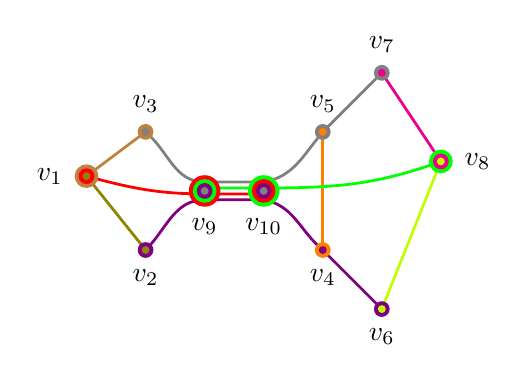
\begin{tikzpicture}  [scale=0.75]
\newdimen\ms
\ms=0.1cm

\tikzstyle{every path}=[line width=1pt]
\tikzstyle{c4}=[circle,inner sep={\ms/8},minimum size=4*\ms]
\tikzstyle{c3}=[circle,inner sep={\ms/8},minimum size=3*\ms]
\tikzstyle{c2}=[circle,inner sep={\ms/8},minimum size=2*\ms]
\tikzstyle{c1}=[circle,inner sep={\ms/8},minimum size=1*\ms]

% Radius of regular polygons
\newdimen\R
\R=5cm
%\r= { \R * sqrt(3)/2}
\newdimen\S
\S=2.5cm

% Define positions of all observables
\path
  (0,0.25) coordinate(1)
  (1,1) coordinate(3)
  (1,-1) coordinate(2)
  (4,-1) coordinate(4)
  (4,1) coordinate(5)
  (5,-2) coordinate(6)
  (5,2) coordinate(7)
  (6,0.5) coordinate(8)
%
  (2,0) coordinate(9)
  (2,-0.15) coordinate(14)
  (2,0.15) coordinate(12)
%
  (3,0) coordinate(10)
  (3,0.15) coordinate(11)
  (3,-0.15) coordinate(13)
%
  (3,0.05) coordinate(15)
  (2,-0.2) coordinate(16)
    (2,0.05) coordinate(19)
  (3,0.3) coordinate(20)
    (2,0.15) coordinate(29)
  (3,0.40) coordinate(30)
    (2,0.05) coordinate(39)
  (3,0.05) coordinate(40)
    (2,-0.05) coordinate(49)
  (3,-0.05) coordinate(50)
;

% draw contexts

\draw [color=olive] (1) -- (2);
\draw [color=brown] (1) -- (3);
\draw [color=violet] (2)  to   [out=45,in=180] (14) -- (13) to [out=-10,in=140] (4) -- (6);
\draw [color=gray] (3)  to [out=320,in=180]  (12) -- (11)  to [out= 10,in=230]  (5) -- (7);
\draw [color=orange] (4) -- (5);
\draw [color=magenta] (7) -- (8);
\draw [color=lime] (6) -- (8);
\draw [color=red] (1) to [out=-15,in=180] (49)  -- (50);
\draw [color=green] (39) -- (40) to [out=0,in=200]  (8);

%
%%
%% draw atoms
%%
%
 \draw (1) coordinate[c3,fill=brown,label=180:$v_1$];
 \draw (1) coordinate[c2,fill=red];
 \draw (1) coordinate[c1,fill=olive];
 %
 \draw (2) coordinate[c2,fill=violet,label=270:$v_2$];
 \draw (2) coordinate[c1,fill=olive];
 %
 \draw (3) coordinate[c2,fill=brown,label=90:$v_3$];
 \draw (3) coordinate[c1,fill=gray];
 %
 \draw (4) coordinate[c2,fill=orange,label=270:$v_4$];
 \draw (4) coordinate[c1,fill=violet];
 %
 \draw (5) coordinate[c2,fill=gray,label=90:$v_5$];
 \draw (5) coordinate[c1,fill=orange];
 %
 \draw (6) coordinate[c2,fill=violet,label=270:$v_6$];
 \draw (6) coordinate[c1,fill=lime];
 %
 %\draw (7) coordinate[c3,fill=orange];
 \draw (7) coordinate[c2,fill=gray,label=90:$v_7$];
 \draw (7) coordinate[c1,fill=magenta];
 %
 \draw (8) coordinate[c3,fill=green,label=0:$v_8$];
 \draw (8) coordinate[c2,fill=magenta];
 \draw (8) coordinate[c1,fill=lime];

 %\draw (8) coordinate[c1,fill=red];
 %
 \draw (10) coordinate[c4,fill=green,label=270:$v_{10}$];
  \draw (10) coordinate[c3,fill=red];
 \draw (10) coordinate[c2,fill=violet];
 \draw (10) coordinate[c1,fill=gray];

 \draw (9) coordinate[c4,fill=red,label=270:$v_9$];
   \draw (9) coordinate[c3,fill=green];
 \draw (9) coordinate[c2,fill=violet];
 \draw (9) coordinate[c1,fill=gray];
%%
%\draw (10) coordinate[c2,fill=brown];
%\draw (10) coordinate[c1,fill=brown];
%%
%\draw (11) coordinate[c2,fill=brown];
%\draw (11) coordinate[c1,fill=red];
%%
%\draw (12) coordinate[c1,fill=red];
%%
%\draw (13) coordinate[c1,fill=lime];
%%
%\draw (14) coordinate[c2,fill=orange,label=0:$\quad 7$];
%\draw (14) coordinate[c1,fill=cyan];

\end{tikzpicture}
%%%%%%%%%%%%%%%%%%%%%%%%%%%%%%%%%%%%%%%%%%%%%%%%%%%%%%%%%%%%%%%%%%%%%%%%%%%%
\\  (c) & (d) \\
%%%%%%%%%%%%%%%%%%%%%%%%%%%%%%%%%%%%%%%%%%%%%%%%%%%%%%%%%%%%%%%%%%%%%%%%%%%%
\end{tabular}
\end{center}
\caption{\label{fig:d5}
(Color online)
Orthogonality diagram of the  the four  simplest known~\cite{}
TIFS  in $d=5$, with 9 contexts and 10 atomic propositions.
It is realizable in  $S^4$ by taking,
for instance,
(a)
$v_1     =  (\sqrt{1-\varepsilon^2} / \sqrt{3})(  {0,-1,\sqrt{2},0,0}  )+\varepsilon({0,0,0,0,1})$,
$v_2     = (  {1,0,0,0,0}    )$,
$v_3     = (  {1,\sqrt{2},1,0,0}   )/ 2 $,
$v_4     = (  {0,1,0,0,0}    ) $,
$v_5     = (  {1,0,-1,0,0}     )/\sqrt{2}$,
$v_6     = (  {0,0,1,0,0}     ) $,
$v_7   = (     {-1,\sqrt{2},-1,0,0} )/ 2$,
$v_8   =      (\sqrt{1-\varepsilon^2} / \sqrt{3})  ({\sqrt{2},1,0,0,0})+\varepsilon({0,0,0,1,0})$,
$v_9     = (   {0,0,0,1,0} )$,
$v_{10}     = (   {0,0,0,0,1} )$,
(b)
$v_1     =   (  {0,-1,\sqrt{2},0,0,}  )/\sqrt{3}$,
$v_8   =  (\sqrt{1-\varepsilon^2} / \sqrt{3})  ({\sqrt{2},1,0,0,0})+\varepsilon({0,0,0,1,0})$,
(c)
$v_1     =   (\sqrt{1-\varepsilon^2} / \sqrt{3})(  {0,-1,\sqrt{2},0,0}  )+\varepsilon({0,0,0,1,0})$,
$v_8   =  (        {\sqrt{2},1,0,0,0} )/\sqrt{3}$,
(d)
$v_1     = (  {0,-1,\sqrt{2},0,0}  )/\sqrt{3}$,
$v_8   =  (        {\sqrt{2},1,0,0,0} ) /\sqrt{3}$.
Values on $v_1$ and $v_8$ cannot both be 1, as this would imply the values on $v_2=v_3=v_6=v_7=v_9=v_{10}=v_{11}$ to vanish,
which in turn would require both values $v_4=v_5$ to be 1; which contradicts exclusivity
because those observables belong to the same context and are orthogonal.
In QT, the proposition $v_i$ is represented by the projector $| v_i \rangle\langle v_i |$.
\jr{CORRECTED FIGURE (a) FOR SIMILAR COLORS TO OTHER FIGURES}}
\end{figure*}


\section{Dimension 6}


\jr{There are eight TIFS with a minimum number of propositions in dimension $6$. They are shown in Fig~\ref{fig:d6}.}

\jr{TIPS: (a) The orthogonal representation il (almost) unique (b) Explain the eight graphs and (c) generalize to higher dimensions}

\meil{\textsc{this paragraph can be full rewritten. wrong formulae. must be  $\binom{d-1}{2}=(d-1)(d-2)/2$-2 for $d\geq 5$} Para contar los grafos TITS con menor n\'umero de v\'ertices, basta con contar las posibles conexiones (excepto isomorfismos) entre los v\'ertices del $K_{d-3}$ interior
    y los v\'ertices  TRUE y FALSE. (NOTA: ?`se puede aprovechar alguna de las figuras?). Como cada v\'ertice del $K_{d-3}$ puede tener
    $3$ estados diferentes e incompatibles (adyacente s\'olo a TRUE, adyacente s\'olo a FALSE o adyacente a ambos), tenemos
    combinaciones con repetici\'on de 3 elementos tomados en grupos de $d-3$. F\'ormulas:
    $ \left(\!\!{3\choose {d-3}}\!\!\right)= \binom{d-1}{d-3} = \binom{d-1}{2}=(d-1)(d-2)/2$.}

%%%%%%%%%%%%%%%%%%%%%%%%%%%%%%%%%%%%%%%%%%%%%%%%%%%%%%%%%%%%%%%%%%%
% Fig. NN-28
%%%%%%%%%%%%%%%%%%%%%%%%%%%%%%%%%%%%%%%%%%%%%%%%%%%%%%%%%%%%%%%%%%%
\begin{figure*}
\begin{center}
\begin{tabular}{cc}
%%%%%%%%%%%%%%%%%%%%%%%%%%%%%%%%%%%%%%%%%%%%%%%%%%%%%%%%%%%%%%%%%%%%%%%%%%%%
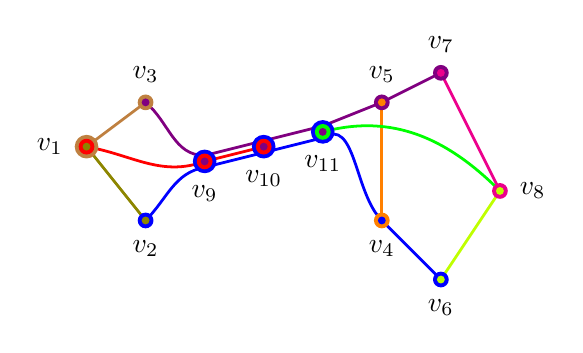
\begin{tikzpicture}  [scale=0.75]
\newdimen\ms
\ms=0.1cm

\tikzstyle{every path}=[line width=1pt]
\tikzstyle{c3}=[circle,inner sep={\ms/8},minimum size=3*\ms]
\tikzstyle{c2}=[circle,inner sep={\ms/8},minimum size=2*\ms]
\tikzstyle{c1}=[circle,inner sep={\ms/8},minimum size=1*\ms]

% Define positions of all observables
\path
  (0,0.25) coordinate(1)
  (1,1) coordinate(3)
  (1,-1) coordinate(2)
  (5,-1) coordinate(4)
  (5,1) coordinate(5)
  (6,-2) coordinate(6)
  (6,1.5) coordinate(7)
  (7,-0.5) coordinate(8)
  (2,0) coordinate(9)
  (3,0.25) coordinate(10)
  (4,0.5) coordinate(11)
  (3,0.35) coordinate(20)
  (2,0.1) coordinate (19)
    (4,0.6) coordinate(21)
  (3,0.15) coordinate(30)
  (2,-0.1) coordinate(29)
    (4,0.4) coordinate(31);

% draw contexts

\draw [color=olive] (1) -- (2);
\draw [color=brown] (1) -- (3);
\draw [color=violet] (3)  to [out=320,in=180] (19) -- (20) -- (21) -- (5) -- (7);
\draw [color=blue] (2)  to   [out=45,in=-170]  (29) -- (30) -- (31) to [out=33] (4) -- (6);
\draw [color=orange] (4) -- (5);
\draw [color=magenta] (7) -- (8);
\draw [color=red] (1) to [out=-10,in=-160] (9) --(10) ;
\draw [color=lime] (6) -- (8);
\draw [color=green] (11) to [out=15] (8);

%
%%
%% draw atoms
%%
%
 \draw (1) coordinate[c3,fill=brown,label=180:$v_1$];
 \draw (1) coordinate[c2,fill=red];
 \draw (1) coordinate[c1,fill=olive];
 %
 \draw (2) coordinate[c2,fill=blue,label=270:$v_2$];
 \draw (2) coordinate[c1,fill=olive];
 %
 \draw (3) coordinate[c2,fill=brown,label=90:$v_3$];
 \draw (3) coordinate[c1,fill=violet];
 %
 \draw (4) coordinate[c2,fill=orange,label=270:$v_4$];
 \draw (4) coordinate[c1,fill=blue];
 %
 \draw (5) coordinate[c2,fill=violet,label=90:$v_5$];
 \draw (5) coordinate[c1,fill=orange];
 %
 \draw (6) coordinate[c2,fill=blue,label=270:$v_6$];
 \draw (6) coordinate[c1,fill=lime];
 %
 %\draw (7) coordinate[c3,fill=orange];
 \draw (7) coordinate[c2,fill=violet,label=90:$v_7$];
 \draw (7) coordinate[c1,fill=magenta];
 %
 \draw (8) coordinate[c2,fill=magenta,label=0:$v_8$];
 \draw (8) coordinate[c1,fill=lime];

 %\draw (8) coordinate[c1,fill=red];
 %
 \draw (10) coordinate[c3,fill=blue,label=270:$v_{10}$];
 \draw (10) coordinate[c2,fill=red];
 \draw (10) coordinate[c1,fill=violet];

 \draw (9) coordinate[c3,fill=blue,label=270:$v_9$];
 \draw (9) coordinate[c2,fill=red];
 \draw (9) coordinate[c1,fill=violet];

  \draw (11) coordinate[c3,fill=blue,label=270:$v_{11}$];
 \draw (11) coordinate[c2,fill=green];
 \draw (11) coordinate[c1,fill=violet];
%%
%\draw (10) coordinate[c2,fill=brown];
%\draw (10) coordinate[c1,fill=brown];
%%
%\draw (29) coordinate[c2,fill=brown];
%\draw (29) coordinate[c1,fill=red];
%%
%\draw (30) coordinate[c1,fill=red];
%%
%\draw (20) coordinate[c1,fill=lime];
%%
%\draw (19) coordinate[c2,fill=orange,label=0:$\quad 7$];
%\draw (19) coordinate[c1,fill=cyan];

\end{tikzpicture}
%%%%%%%%%%%%%%%%%%%%%%%%%%%%%%%%%%%%%%%%%%%%%%%%%%%%%%%%%%%%%%%%%%%%%%%%%%%%
%\\  (a) \\
&
%%%%%%%%%%%%%%%%%%%%%%%%%%%%%%%%%%%%%%%%%%%%%%%%%%%%%%%%%%%%%%%%%%%%%%%%%%%%
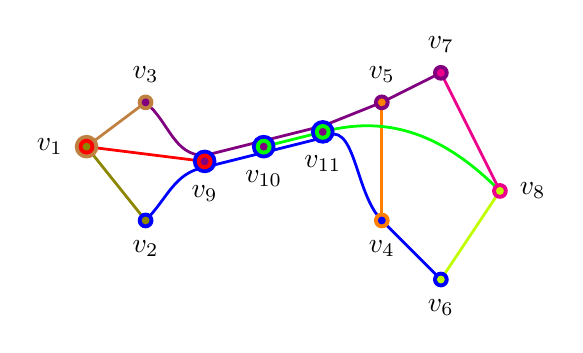
\begin{tikzpicture}  [scale=0.75]
\newdimen\ms
\ms=0.1cm

\tikzstyle{every path}=[line width=1pt]
\tikzstyle{c3}=[circle,inner sep={\ms/8},minimum size=3*\ms]
\tikzstyle{c2}=[circle,inner sep={\ms/8},minimum size=2*\ms]
\tikzstyle{c1}=[circle,inner sep={\ms/8},minimum size=1*\ms]

% Define positions of all observables
\path
  (0,0.25) coordinate(1)
  (1,1) coordinate(3)
  (1,-1) coordinate(2)
  (5,-1) coordinate(4)
  (5,1) coordinate(5)
  (6,-2) coordinate(6)
  (6,1.5) coordinate(7)
  (7,-0.5) coordinate(8)
  (2,0) coordinate(9)
  (3,0.25) coordinate(10)
  (4,0.5) coordinate(11)
  (3,0.35) coordinate(20)
  (2,0.1) coordinate (19)
    (4,0.6) coordinate(21)
  (3,0.15) coordinate(30)
  (2,-0.1) coordinate(29)
    (4,0.4) coordinate(31);

% draw contexts

\draw [color=olive] (1) -- (2);
\draw [color=brown] (1) -- (3);
\draw [color=violet] (3)  to [out=320,in=180] (19) -- (20) -- (21) -- (5) -- (7);
\draw [color=blue] (2)  to   [out=45,in=-170]  (29) -- (30) -- (31) to [out=33] (4) -- (6);
\draw [color=orange] (4) -- (5);
\draw [color=magenta] (7) -- (8);
\draw [color=red] (1) -- (9) ;
\draw [color=lime] (6) -- (8);
\draw [color=green] (10) -- (11) to [out=15] (8);

%
%%
%% draw atoms
%%
%
 \draw (1) coordinate[c3,fill=brown,label=180:$v_1$];
 \draw (1) coordinate[c2,fill=red];
 \draw (1) coordinate[c1,fill=olive];
 %
 \draw (2) coordinate[c2,fill=blue,label=270:$v_2$];
 \draw (2) coordinate[c1,fill=olive];
 %
 \draw (3) coordinate[c2,fill=brown,label=90:$v_3$];
 \draw (3) coordinate[c1,fill=violet];
 %
 \draw (4) coordinate[c2,fill=orange,label=270:$v_4$];
 \draw (4) coordinate[c1,fill=blue];
 %
 \draw (5) coordinate[c2,fill=violet,label=90:$v_5$];
 \draw (5) coordinate[c1,fill=orange];
 %
 \draw (6) coordinate[c2,fill=blue,label=270:$v_6$];
 \draw (6) coordinate[c1,fill=lime];
 %
 %\draw (7) coordinate[c3,fill=orange];
 \draw (7) coordinate[c2,fill=violet,label=90:$v_7$];
 \draw (7) coordinate[c1,fill=magenta];
 %
 \draw (8) coordinate[c2,fill=magenta,label=0:$v_8$];
 \draw (8) coordinate[c1,fill=lime];

 %\draw (8) coordinate[c1,fill=red];
 %
 \draw (10) coordinate[c3,fill=blue,label=270:$v_{10}$];
 \draw (10) coordinate[c2,fill=green];
 \draw (10) coordinate[c1,fill=violet];

 \draw (9) coordinate[c3,fill=blue,label=270:$v_9$];
 \draw (9) coordinate[c2,fill=red];
 \draw (9) coordinate[c1,fill=violet];

  \draw (11) coordinate[c3,fill=blue,label=270:$v_{11}$];
 \draw (11) coordinate[c2,fill=green];
 \draw (11) coordinate[c1,fill=violet];
%%
%\draw (10) coordinate[c2,fill=brown];
%\draw (10) coordinate[c1,fill=brown];
%%
%\draw (29) coordinate[c2,fill=brown];
%\draw (29) coordinate[c1,fill=red];
%%
%\draw (30) coordinate[c1,fill=red];
%%
%\draw (20) coordinate[c1,fill=lime];
%%
%\draw (19) coordinate[c2,fill=orange,label=0:$\quad 7$];
%\draw (19) coordinate[c1,fill=cyan];

\end{tikzpicture}
%%%%%%%%%%%%%%%%%%%%%%%%%%%%%%%%%%%%%%%%%%%%%%%%%%%%%%%%%%%%%%%%%%%%%%%%%%%%
\\ (a) &  (b) \\
% (b)
%%%%%%%%%%%%%%%%%%%%%%%%%%%%%%%%%%%%%%%%%%%%%%%%%%%%%%%%%%%%%%%%%%%%%%%%%%%%%%%%%%%%%%%%%%%%%%%%%%%%%%%%%%%%%%%%%%%%%%%%%%%%%%%%%%%%%%%%%%%%%%%%%%%%%%%%%
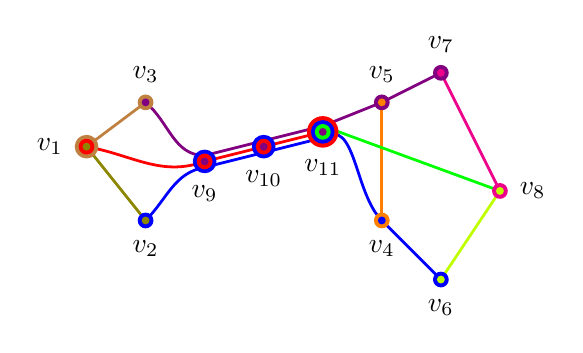
\begin{tikzpicture}  [scale=0.75]
\newdimen\ms
\ms=0.1cm

\tikzstyle{every path}=[line width=1pt]
\tikzstyle{c4}=[circle,inner sep={\ms/8},minimum size=4*\ms]
\tikzstyle{c3}=[circle,inner sep={\ms/8},minimum size=3*\ms]
\tikzstyle{c2}=[circle,inner sep={\ms/8},minimum size=2*\ms]
\tikzstyle{c1}=[circle,inner sep={\ms/8},minimum size=1*\ms]

% Define positions of all observables
\path
  (0,0.25) coordinate(1)
  (1,1) coordinate(3)
  (1,-1) coordinate(2)
  (5,-1) coordinate(4)
  (5,1) coordinate(5)
  (6,-2) coordinate(6)
  (6,1.5) coordinate(7)
  (7,-0.5) coordinate(8)
  (2,0) coordinate(9)
  (3,0.25) coordinate(10)
  (4,0.5) coordinate(11)
  (3,0.35) coordinate(20)
  (2,0.1) coordinate (19)
    (4,0.6) coordinate(21)
  (3,0.15) coordinate(30)
  (2,-0.1) coordinate(29)
    (4,0.4) coordinate(31);

% draw contexts

\draw [color=olive] (1) -- (2);
\draw [color=brown] (1) -- (3);
\draw [color=violet] (3)  to [out=320,in=180] (19) -- (20) -- (21) -- (5) -- (7);
\draw [color=blue] (2)  to   [out=45,in=-170]  (29) -- (30) -- (31)  to [out=33] (4) -- (6);
\draw [color=orange] (4) -- (5);
\draw [color=magenta] (7) -- (8);
\draw [color=red] (1) to [out=-10,in=-160] (9) --(10) -- (11) ;
\draw [color=lime] (6) -- (8);
\draw [color=green] (21) -- (8);

%
%%
%% draw atoms
%%
%
 \draw (1) coordinate[c3,fill=brown,label=180:$v_1$];
 \draw (1) coordinate[c2,fill=red];
 \draw (1) coordinate[c1,fill=olive];
 %
 \draw (2) coordinate[c2,fill=blue,label=270:$v_2$];
 \draw (2) coordinate[c1,fill=olive];
 %
 \draw (3) coordinate[c2,fill=brown,label=90:$v_3$];
 \draw (3) coordinate[c1,fill=violet];
 %
 \draw (4) coordinate[c2,fill=orange,label=270:$v_4$];
 \draw (4) coordinate[c1,fill=blue];
 %
 \draw (5) coordinate[c2,fill=violet,label=90:$v_5$];
 \draw (5) coordinate[c1,fill=orange];
 %
 \draw (6) coordinate[c2,fill=blue,label=270:$v_6$];
 \draw (6) coordinate[c1,fill=lime];
 %
 %\draw (7) coordinate[c3,fill=orange];
 \draw (7) coordinate[c2,fill=violet,label=90:$v_7$];
 \draw (7) coordinate[c1,fill=magenta];
 %
 \draw (8) coordinate[c2,fill=magenta,label=0:$v_8$];
 \draw (8) coordinate[c1,fill=lime];

 %\draw (8) coordinate[c1,fill=red];
 %

 \draw (9) coordinate[c3,fill=blue,label=270:$v_9$];
 \draw (9) coordinate[c2,fill=red];
 \draw (9) coordinate[c1,fill=violet];

  \draw (10) coordinate[c3,fill=blue,label=270:$v_{10}$];
 \draw (10) coordinate[c2,fill=red];
 \draw (10) coordinate[c1,fill=violet];

  \draw (11) coordinate[c4,fill=red,label=270:$v_{11}$];
 \draw (11) coordinate[c3,fill=blue];
 \draw (11) coordinate[c2,fill=green];
 \draw (11) coordinate[c1,fill=violet];
%%
%\draw (10) coordinate[c2,fill=brown];
%\draw (10) coordinate[c1,fill=brown];
%%
%\draw (29) coordinate[c2,fill=brown];
%\draw (29) coordinate[c1,fill=red];
%%
%\draw (30) coordinate[c1,fill=red];
%%
%\draw (20) coordinate[c1,fill=lime];
%%
%\draw (19) coordinate[c2,fill=orange,label=0:$\quad 7$];
%\draw (19) coordinate[c1,fill=cyan];

\end{tikzpicture}
%%%%%%%%%%%%%%%%%%%%%%%%%%%%%%%%%%%%%%%%%%%%%%%%%%%%%%%%%%%%%%%%%%%%%%%%%%%%
%\\  (c) \\
&
%%%%%%%%%%%%%%%%%%%%%%%%%%%%%%%%%%%%%%%%%%%%%%%%%%%%%%%%%%%%%%%%%%%%%%%%%%%%
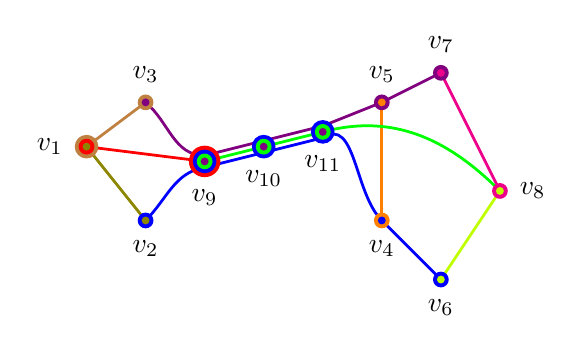
\begin{tikzpicture}  [scale=0.75]
\newdimen\ms
\ms=0.1cm

\tikzstyle{every path}=[line width=1pt]
\tikzstyle{c4}=[circle,inner sep={\ms/8},minimum size=4*\ms]
\tikzstyle{c3}=[circle,inner sep={\ms/8},minimum size=3*\ms]
\tikzstyle{c2}=[circle,inner sep={\ms/8},minimum size=2*\ms]
\tikzstyle{c1}=[circle,inner sep={\ms/8},minimum size=1*\ms]

% Define positions of all observables
\path
  (0,0.25) coordinate(1)
  (1,1) coordinate(3)
  (1,-1) coordinate(2)
  (5,-1) coordinate(4)
  (5,1) coordinate(5)
  (6,-2) coordinate(6)
  (6,1.5) coordinate(7)
  (7,-0.5) coordinate(8)
  (2,0) coordinate(9)
  (3,0.25) coordinate(10)
  (4,0.5) coordinate(11)
  (3,0.35) coordinate(20)
  (2,0.1) coordinate (19)
    (4,0.6) coordinate(21)
  (3,0.15) coordinate(30)
  (2,-0.1) coordinate(29)
    (4,0.4) coordinate(31);

% draw contexts

\draw [color=olive] (1) -- (2);
\draw [color=brown] (1) -- (3);
\draw [color=violet] (3)  to [out=320,in=180] (19) -- (20) -- (21) -- (5) -- (7);
\draw [color=blue] (2)  to   [out=45,in=-170]  (29) -- (30) -- (31) to [out=33] (4) -- (6);
\draw [color=orange] (4) -- (5);
\draw [color=magenta] (7) -- (8);
\draw [color=red] (1) -- (9) ;
\draw [color=lime] (6) -- (8);
\draw [color=green] (9) -- (10) -- (11) to [out=15] (8);

%
%%
%% draw atoms
%%
%
 \draw (1) coordinate[c3,fill=brown,label=180:$v_1$];
 \draw (1) coordinate[c2,fill=red];
 \draw (1) coordinate[c1,fill=olive];
 %
 \draw (2) coordinate[c2,fill=blue,label=270:$v_2$];
 \draw (2) coordinate[c1,fill=olive];
 %
 \draw (3) coordinate[c2,fill=brown,label=90:$v_3$];
 \draw (3) coordinate[c1,fill=violet];
 %
 \draw (4) coordinate[c2,fill=orange,label=270:$v_4$];
 \draw (4) coordinate[c1,fill=blue];
 %
 \draw (5) coordinate[c2,fill=violet,label=90:$v_5$];
 \draw (5) coordinate[c1,fill=orange];
 %
 \draw (6) coordinate[c2,fill=blue,label=270:$v_6$];
 \draw (6) coordinate[c1,fill=lime];
 %
 %\draw (7) coordinate[c3,fill=orange];
 \draw (7) coordinate[c2,fill=violet,label=90:$v_7$];
 \draw (7) coordinate[c1,fill=magenta];
 %
 \draw (8) coordinate[c2,fill=magenta,label=0:$v_8$];
 \draw (8) coordinate[c1,fill=lime];

 %\draw (8) coordinate[c1,fill=red];
 %

  \draw (9) coordinate[c4,fill=red,label=270:$v_9$];
 \draw (9) coordinate[c3,fill=blue];
 \draw (9) coordinate[c2,fill=green];
 \draw (9) coordinate[c1,fill=violet];

  \draw (10) coordinate[c3,fill=blue,label=270:$v_{10}$];
 \draw (10) coordinate[c2,fill=green];
 \draw (10) coordinate[c1,fill=violet];


  \draw (11) coordinate[c3,fill=blue,label=270:$v_{11}$];
 \draw (11) coordinate[c2,fill=green];
 \draw (11) coordinate[c1,fill=violet];
%%
%\draw (10) coordinate[c2,fill=brown];
%\draw (10) coordinate[c1,fill=brown];
%%
%\draw (29) coordinate[c2,fill=brown];
%\draw (29) coordinate[c1,fill=red];
%%
%\draw (30) coordinate[c1,fill=red];
%%
%\draw (20) coordinate[c1,fill=lime];
%%
%\draw (19) coordinate[c2,fill=orange,label=0:$\quad 7$];
%\draw (19) coordinate[c1,fill=cyan];

\end{tikzpicture}
%%%%%%%%%%%%%%%%%%%%%%%%%%%%%%%%%%%%%%%%%%%%%%%%%%%%%%%%%%%%%%%%%%%%%%%%%%%%
\\  (c) & (d) \\
%%%%%%%%%%%%%%%%%%%%%%%%%%%%%%%%%%%%%%%%%%%%%%%%%%%%%%%%%%%%%%%%%%%%%%%%%%%%%%%%%%%%%%%%%%%%%%%%%%%%%%%%%%%%%%%%%%%%%%%%%%%%%%%%%%%%%%%%%%%%%%%%%%%%%%%%
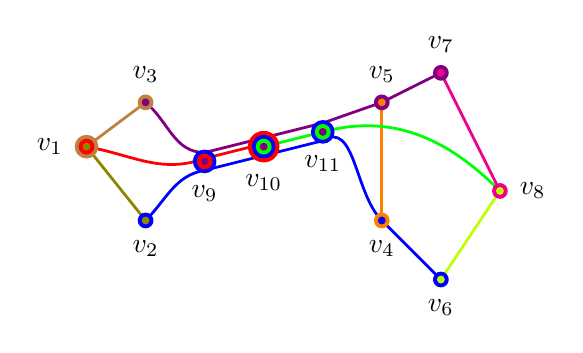
\begin{tikzpicture}  [scale=0.75]
\newdimen\ms
\ms=0.1cm

\tikzstyle{every path}=[line width=1pt]
\tikzstyle{c4}=[circle,inner sep={\ms/8},minimum size=4*\ms]
\tikzstyle{c3}=[circle,inner sep={\ms/8},minimum size=3*\ms]
\tikzstyle{c2}=[circle,inner sep={\ms/8},minimum size=2*\ms]
\tikzstyle{c1}=[circle,inner sep={\ms/8},minimum size=1*\ms]

% Define positions of all observables
\path
  (0,0.25) coordinate(1)
  (1,1) coordinate(3)
  (1,-1) coordinate(2)
  (5,-1) coordinate(4)
  (5,1) coordinate(5)
  (6,-2) coordinate(6)
  (6,1.5) coordinate(7)
  (7,-0.5) coordinate(8)
  (2,0) coordinate(9)
  (3,0.25) coordinate(10)
  (4,0.5) coordinate(11)
  (2,0.05) coordinate(19)
  (3,0.30) coordinate(20)
  (4,0.55) coordinate(21)
  (2,0.15) coordinate(29)
  (3,0.4) coordinate(30)
  (4,0.65) coordinate(31)
  (2,-0.05) coordinate(39)
  (3,0.2) coordinate(40)
  (4,0.45) coordinate(41)
  (2,-0.15) coordinate(49)
  (3,0.1) coordinate(50)
  (4,0.35) coordinate(51);

% draw contexts

\draw [color=olive] (1) -- (2);
\draw [color=brown] (1) -- (3);
\draw [color=violet] (3)  to [out=320,in=180]  (29) --(30) -- (31) -- (5) -- (7);
\draw [color=blue] (2)  to   [out=45,in=-170]   (49) -- (50) -- (51) to [out=33] (4) -- (6);
\draw [color=orange] (4) -- (5);
\draw [color=magenta] (7) -- (8);
\draw [color=red] (1) to [out=-10,in=-160] (19) -- (20);
\draw [color=lime] (6) -- (8);
\draw [color=green] (10) -- (11) to [out=15] (8);

%
%%
%% draw atoms
%%
%
 \draw (1) coordinate[c3,fill=brown,label=180:$v_1$];
 \draw (1) coordinate[c2,fill=red];
 \draw (1) coordinate[c1,fill=olive];
 %
 \draw (2) coordinate[c2,fill=blue,label=270:$v_2$];
 \draw (2) coordinate[c1,fill=olive];
 %
 \draw (3) coordinate[c2,fill=brown,label=90:$v_3$];
 \draw (3) coordinate[c1,fill=violet];
 %
 \draw (4) coordinate[c2,fill=orange,label=270:$v_4$];
 \draw (4) coordinate[c1,fill=blue];
 %
 \draw (5) coordinate[c2,fill=violet,label=90:$v_5$];
 \draw (5) coordinate[c1,fill=orange];
 %
 \draw (6) coordinate[c2,fill=blue,label=270:$v_6$];
 \draw (6) coordinate[c1,fill=lime];
 %
 %\draw (7) coordinate[c3,fill=orange];
 \draw (7) coordinate[c2,fill=violet,label=90:$v_7$];
 \draw (7) coordinate[c1,fill=magenta];
 %
 \draw (8) coordinate[c2,fill=magenta,label=0:$v_8$];
 \draw (8) coordinate[c1,fill=lime];

 %\draw (8) coordinate[c1,fill=red];
 %


  \draw (9) coordinate[c3,fill=blue,label=270:$v_9$];
 \draw (9) coordinate[c2,fill=red];
 \draw (9) coordinate[c1,fill=violet];

   \draw (10) coordinate[c4,fill=red,label=270:$v_{10}$];
    \draw (10) coordinate[c3,fill=blue];
 \draw (10) coordinate[c2,fill=green];
 \draw (10) coordinate[c1,fill=violet];

 \draw (11) coordinate[c3,fill=blue,label=270:$v_{11}$];
 \draw (11) coordinate[c2,fill=green];
 \draw (11) coordinate[c1,fill=violet];
%%
%\draw (10) coordinate[c2,fill=brown];
%\draw (10) coordinate[c1,fill=brown];
%%
%\draw (29) coordinate[c2,fill=brown];
%\draw (29) coordinate[c1,fill=red];
%%
%\draw (30) coordinate[c1,fill=red];
%%
%\draw (20) coordinate[c1,fill=lime];
%%
%\draw (19) coordinate[c2,fill=orange,label=0:$\quad 7$];
%\draw (19) coordinate[c1,fill=cyan];

\end{tikzpicture}
%%%%%%%%%%%%%%%%%%%%%%%%%%%%%%%%%%%%%%%%%%%%%%%%%%%%%%%%%%%%%%%%%%%%%%%%%%%%
& %(e) \\
%%%%%%%%%%%%%%%%%%%%%%%%%%%%%%%%%%%%%%%%%%%%%%%%%%%%%%%%%%%%%%%%%%%%%%%%%%%%%%%%%%%%%%%%%%%%%%%%%%%%%%%%%%%%%%%%%%%%%%%%%%%%%%%%%%%%%%%%%%%%%%%%%%%%%%%%
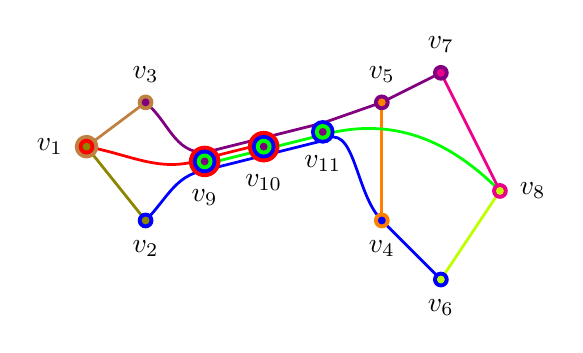
\begin{tikzpicture}  [scale=0.75]
\newdimen\ms
\ms=0.1cm

\tikzstyle{every path}=[line width=1pt]
\tikzstyle{c4}=[circle,inner sep={\ms/8},minimum size=4*\ms]
\tikzstyle{c3}=[circle,inner sep={\ms/8},minimum size=3*\ms]
\tikzstyle{c2}=[circle,inner sep={\ms/8},minimum size=2*\ms]
\tikzstyle{c1}=[circle,inner sep={\ms/8},minimum size=1*\ms]

% Define positions of all observables
\path
  (0,0.25) coordinate(1)
  (1,1) coordinate(3)
  (1,-1) coordinate(2)
  (5,-1) coordinate(4)
  (5,1) coordinate(5)
  (6,-2) coordinate(6)
  (6,1.5) coordinate(7)
  (7,-0.5) coordinate(8)
  (2,0) coordinate(9)
  (3,0.25) coordinate(10)
  (4,0.5) coordinate(11)
  (2,0.05) coordinate(19)
  (3,0.30) coordinate(20)
  (4,0.55) coordinate(21)
  (2,0.15) coordinate(29)
  (3,0.4) coordinate(30)
  (4,0.65) coordinate(31)
  (2,-0.05) coordinate(39)
  (3,0.2) coordinate(40)
  (4,0.45) coordinate(41)
  (2,-0.15) coordinate(49)
  (3,0.1) coordinate(50)
  (4,0.35) coordinate(51);

% draw contexts

\draw [color=olive] (1) -- (2);
\draw [color=brown] (1) -- (3);
\draw [color=violet] (3)  to [out=320,in=180]  (29) --(30) -- (31) -- (5) -- (7);
\draw [color=blue] (2)  to   [out=45,in=-170]  (49) -- (50) -- (51) to [out=33] (4) -- (6);
\draw [color=orange] (4) -- (5);
\draw [color=magenta] (7) -- (8);
\draw [color=red] (1) to [out=-10,in=-160] (19) -- (20);
\draw [color=lime] (6) -- (8);
\draw [color=green] (39) -- (40) -- (41) to [out=15] (8);

%
%%
%% draw atoms
%%
%
 \draw (1) coordinate[c3,fill=brown,label=180:$v_1$];
 \draw (1) coordinate[c2,fill=red];
 \draw (1) coordinate[c1,fill=olive];
 %
 \draw (2) coordinate[c2,fill=blue,label=270:$v_2$];
 \draw (2) coordinate[c1,fill=olive];
 %
 \draw (3) coordinate[c2,fill=brown,label=90:$v_3$];
 \draw (3) coordinate[c1,fill=violet];
 %
 \draw (4) coordinate[c2,fill=orange,label=270:$v_4$];
 \draw (4) coordinate[c1,fill=blue];
 %
 \draw (5) coordinate[c2,fill=violet,label=90:$v_5$];
 \draw (5) coordinate[c1,fill=orange];
 %
 \draw (6) coordinate[c2,fill=blue,label=270:$v_6$];
 \draw (6) coordinate[c1,fill=lime];
 %
 %\draw (7) coordinate[c3,fill=orange];
 \draw (7) coordinate[c2,fill=violet,label=90:$v_7$];
 \draw (7) coordinate[c1,fill=magenta];
 %
 \draw (8) coordinate[c2,fill=magenta,label=0:$v_8$];
 \draw (8) coordinate[c1,fill=lime];

 %\draw (8) coordinate[c1,fill=red];
 %


 \draw (9) coordinate[c4,fill=red,label=270:$v_{9}$];
 \draw (9) coordinate[c3,fill=blue];
 \draw (9) coordinate[c2,fill=green];
 \draw (9) coordinate[c1,fill=violet];

   \draw (10) coordinate[c4,fill=red,label=270:$v_{10}$];
    \draw (10) coordinate[c3,fill=blue];
 \draw (10) coordinate[c2,fill=green];
 \draw (10) coordinate[c1,fill=violet];

 \draw (11) coordinate[c3,fill=blue,label=270:$v_{11}$];
 \draw (11) coordinate[c2,fill=green];
 \draw (11) coordinate[c1,fill=violet];
%%
%\draw (10) coordinate[c2,fill=brown];
%\draw (10) coordinate[c1,fill=brown];
%%
%\draw (29) coordinate[c2,fill=brown];
%\draw (29) coordinate[c1,fill=red];
%%
%\draw (30) coordinate[c1,fill=red];
%%
%\draw (20) coordinate[c1,fill=lime];
%%
%\draw (19) coordinate[c2,fill=orange,label=0:$\quad 7$];
%\draw (19) coordinate[c1,fill=cyan];

\end{tikzpicture}
%%%%%%%%%%%%%%%%%%%%%%%%%%%%%%%%%%%%%%%%%%%%%%%%%%%%%%%%%%%%%%%%%%%%%%%%%%%
\\ (e) & (f) \\
%%%%%%%%%%%%%%%%%%%%%%%%%%%%%%%%%%%%%%%%%%%%%%%%%%%%%%%%%%%%%%%%%%%%%%%%%%%%
%%%%%%%%%%%%%%%%%%%%%%%%%%%%%%%%%%%%%%%%%%%%%%%%%%%%%%%%%%%%%%%%%%%%%%%%%%%
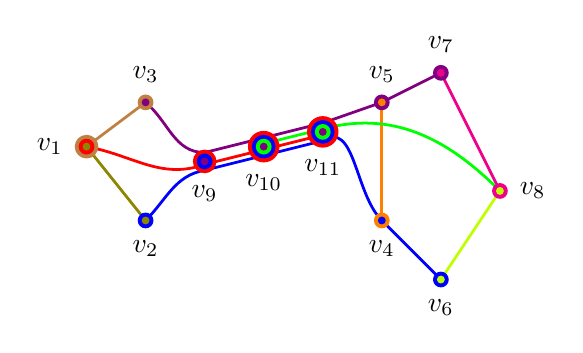
\begin{tikzpicture}  [scale=0.75]
\newdimen\ms
\ms=0.1cm

\tikzstyle{every path}=[line width=1pt]
\tikzstyle{c4}=[circle,inner sep={\ms/8},minimum size=4*\ms]
\tikzstyle{c3}=[circle,inner sep={\ms/8},minimum size=3*\ms]
\tikzstyle{c2}=[circle,inner sep={\ms/8},minimum size=2*\ms]
\tikzstyle{c1}=[circle,inner sep={\ms/8},minimum size=1*\ms]

% Define positions of all observables
\path
  (0,0.25) coordinate(1)
  (1,1) coordinate(3)
  (1,-1) coordinate(2)
  (5,-1) coordinate(4)
  (5,1) coordinate(5)
  (6,-2) coordinate(6)
  (6,1.5) coordinate(7)
  (7,-0.5) coordinate(8)
  (2,0) coordinate(9)
  (3,0.25) coordinate(10)
  (4,0.5) coordinate(11)
  (2,0.05) coordinate(19)
  (3,0.30) coordinate(20)
  (4,0.55) coordinate(21)
  (2,0.15) coordinate(29)
  (3,0.4) coordinate(30)
  (4,0.65) coordinate(31)
  (2,-0.05) coordinate(39)
  (3,0.2) coordinate(40)
  (4,0.45) coordinate(41)
  (2,-0.15) coordinate(49)
  (3,0.1) coordinate(50)
  (4,0.35) coordinate(51);

% draw contexts

\draw [color=olive] (1) -- (2);
\draw [color=brown] (1) -- (3);
\draw [color=violet] (3)  to [out=320,in=180]  (29) --(30) -- (31)  -- (5) -- (7);
\draw [color=blue] (2)  to   [out=45,in=-170]  (49) -- (50) -- (51) to [out=33] (4) -- (6);
\draw [color=orange] (4) -- (5);
\draw [color=magenta] (7) -- (8);
\draw [color=red] (1) to [out=-10,in=-160] (39) --(40) -- (41);
\draw [color=lime] (6) -- (8);
\draw [color=green] (20) -- (21) to [out=15] (8);

%
%%
%% draw atoms
%%
%
 \draw (1) coordinate[c3,fill=brown,label=180:$v_1$];
 \draw (1) coordinate[c2,fill=red];
 \draw (1) coordinate[c1,fill=olive];
 %
 \draw (2) coordinate[c2,fill=blue,label=270:$v_2$];
 \draw (2) coordinate[c1,fill=olive];
 %
 \draw (3) coordinate[c2,fill=brown,label=90:$v_3$];
 \draw (3) coordinate[c1,fill=violet];
 %
 \draw (4) coordinate[c2,fill=orange,label=270:$v_4$];
 \draw (4) coordinate[c1,fill=blue];
 %
 \draw (5) coordinate[c2,fill=violet,label=90:$v_5$];
 \draw (5) coordinate[c1,fill=orange];
 %
 \draw (6) coordinate[c2,fill=blue,label=270:$v_6$];
 \draw (6) coordinate[c1,fill=lime];
 %
 %\draw (7) coordinate[c3,fill=orange];
 \draw (7) coordinate[c2,fill=violet,label=90:$v_7$];
 \draw (7) coordinate[c1,fill=magenta];
 %
 \draw (8) coordinate[c2,fill=magenta,label=0:$v_8$];
 \draw (8) coordinate[c1,fill=lime];

 %\draw (8) coordinate[c1,fill=red];
 %


 \draw (9) coordinate[c3,fill=red,label=270:$v_{9}$];
 \draw (9) coordinate[c2,fill=blue];
 \draw (9) coordinate[c1,fill=violet];

   \draw (10) coordinate[c4,fill=red,label=270:$v_{10}$];
    \draw (10) coordinate[c3,fill=blue];
 \draw (10) coordinate[c2,fill=green];
 \draw (10) coordinate[c1,fill=violet];

   \draw (11) coordinate[c4,fill=red,label=270:$v_{11}$];
    \draw (11) coordinate[c3,fill=blue];
 \draw (11) coordinate[c2,fill=green];
 \draw (11) coordinate[c1,fill=violet];
%%
%\draw (10) coordinate[c2,fill=brown];
%\draw (10) coordinate[c1,fill=brown];
%%
%\draw (29) coordinate[c2,fill=brown];
%\draw (29) coordinate[c1,fill=red];
%%
%\draw (30) coordinate[c1,fill=red];
%%
%\draw (20) coordinate[c1,fill=lime];
%%
%\draw (19) coordinate[c2,fill=orange,label=0:$\quad 7$];
%\draw (19) coordinate[c1,fill=cyan];

\end{tikzpicture}
%%%%%%%%%%%%%%%%%%%%%%%%%%%%%%%%%%%%%%%%%%%%%%%%%%%%%%%%%%%%%%%%%%%%%%%%%%%%
& %(g) \\
%%%%%%%%%%%%%%%%%%%%%%%%%%%%%%%%%%%%%%%%%%%%%%%%%%%%%%%%%%%%%%%%%%%%%%%%%%%%%%%%%%%%%%%%%%%%%%%%%%%%%%%%%%%%%%%%%%%%%%%%%%%%%%%%%%%%%%%%%%%%%%%%%%%%%%%%
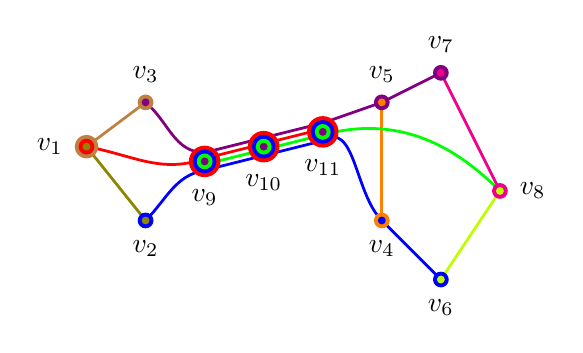
\begin{tikzpicture}  [scale=0.75]
\newdimen\ms
\ms=0.1cm

\tikzstyle{every path}=[line width=1pt]
\tikzstyle{c4}=[circle,inner sep={\ms/8},minimum size=4*\ms]
\tikzstyle{c3}=[circle,inner sep={\ms/8},minimum size=3*\ms]
\tikzstyle{c2}=[circle,inner sep={\ms/8},minimum size=2*\ms]
\tikzstyle{c1}=[circle,inner sep={\ms/8},minimum size=1*\ms]

% Define positions of all observables
\path
  (0,0.25) coordinate(1)
  (1,1) coordinate(3)
  (1,-1) coordinate(2)
  (5,-1) coordinate(4)
  (5,1) coordinate(5)
  (6,-2) coordinate(6)
  (6,1.5) coordinate(7)
  (7,-0.5) coordinate(8)
  (2,0) coordinate(9)
  (3,0.25) coordinate(10)
  (4,0.5) coordinate(11)
  (2,0.05) coordinate(19)
  (3,0.30) coordinate(20)
  (4,0.55) coordinate(21)
  (2,0.15) coordinate(29)
  (3,0.4) coordinate(30)
  (4,0.65) coordinate(31)
  (2,-0.05) coordinate(39)
  (3,0.2) coordinate(40)
  (4,0.45) coordinate(41)
  (2,-0.15) coordinate(49)
  (3,0.1) coordinate(50)
  (4,0.35) coordinate(51);

% draw contexts

\draw [color=olive] (1) -- (2);
\draw [color=brown] (1) -- (3);
\draw [color=violet] (3)  to [out=320,in=180] (29) --(30) -- (31) -- (5) -- (7);
\draw [color=blue] (2)  to   [out=45,in=-170]  (49) -- (50) -- (51) to [out=33] (4) -- (6);
\draw [color=orange] (4) -- (5);
\draw [color=magenta] (7) -- (8);
\draw [color=red] (1) to [out=-10,in=-160] (19) -- (20) -- (21);
\draw [color=lime] (6) -- (8);
\draw [color=green] (39) -- (40) -- (41) to [out=15] (8);

%
%%
%% draw atoms
%%
%
 \draw (1) coordinate[c3,fill=brown,label=180:$v_1$];
 \draw (1) coordinate[c2,fill=red];
 \draw (1) coordinate[c1,fill=olive];
 %
 \draw (2) coordinate[c2,fill=blue,label=270:$v_2$];
 \draw (2) coordinate[c1,fill=olive];
 %
 \draw (3) coordinate[c2,fill=brown,label=90:$v_3$];
 \draw (3) coordinate[c1,fill=violet];
 %
 \draw (4) coordinate[c2,fill=orange,label=270:$v_4$];
 \draw (4) coordinate[c1,fill=blue];
 %
 \draw (5) coordinate[c2,fill=violet,label=90:$v_5$];
 \draw (5) coordinate[c1,fill=orange];
 %
 \draw (6) coordinate[c2,fill=blue,label=270:$v_6$];
 \draw (6) coordinate[c1,fill=lime];
 %
 %\draw (7) coordinate[c3,fill=orange];
 \draw (7) coordinate[c2,fill=violet,label=90:$v_7$];
 \draw (7) coordinate[c1,fill=magenta];
 %
 \draw (8) coordinate[c2,fill=magenta,label=0:$v_8$];
 \draw (8) coordinate[c1,fill=lime];

 %\draw (8) coordinate[c1,fill=red];
 %


\draw (9) coordinate[c4,fill=red,label=270:$v_{9}$];
\draw (9) coordinate[c3,fill=blue];
\draw (9) coordinate[c2,fill=green];
\draw (9) coordinate[c1,fill=violet];

\draw (10) coordinate[c4,fill=red,label=270:$v_{10}$];
\draw (10) coordinate[c3,fill=blue];
\draw (10) coordinate[c2,fill=green];
\draw (10) coordinate[c1,fill=violet];

\draw (11) coordinate[c4,fill=red,label=270:$v_{11}$];
\draw (11) coordinate[c3,fill=blue];
\draw (11) coordinate[c2,fill=green];
\draw (11) coordinate[c1,fill=violet];
%%
%\draw (10) coordinate[c2,fill=brown];
%\draw (10) coordinate[c1,fill=brown];
%%
%\draw (29) coordinate[c2,fill=brown];
%\draw (29) coordinate[c1,fill=red];
%%
%\draw (30) coordinate[c1,fill=red];
%%
%\draw (20) coordinate[c1,fill=lime];
%%
%\draw (19) coordinate[c2,fill=orange,label=0:$\quad 7$];
%\draw (19) coordinate[c1,fill=cyan];

\end{tikzpicture}
\\ (g) & (h) \\
%%%%%%%%%%%%%%%%%%%%%%%%%%%%%%%%%%%%%%%%%%%%%%%%%%%%%%%%%%%%%%%%%%%%%%%%%%%%
\\
%%%%%%%%%%%%%%%%%%%%%%%%%%%%%%%%%%%%%%%%%%%%%%%%%%%%%%%%%%%%%%%%%%%%%%%%%%%%
\end{tabular}
\end{center}
\caption{\label{fig:d6}
(Color online)
see text}

\end{figure*}

%\clearpage

Orthogonality diagram of the  the four  simplest known~\cite{}
TIFS  in $d=6$, with 9 contexts and 11 atomic propositions.
It is realizable in  $S^5$ by taking,
for instance,
(a)
$v_1     =  (\sqrt{1-\varepsilon^2} / \sqrt{3})(  {0,-1,\sqrt{2},0,0,0}  )+\varepsilon({0,0,0,0,0.1})$,
$v_2     = (  {1,0,0,0,0,0}    )$,
$v_3     = (  {1,\sqrt{2},1,0,0,0}   )/ 2 $,
$v_4     = (  {0,1,0,0,0,0}    ) $,
$v_5     = (  {1,0,-1,0,0,0}     )/\sqrt{2}$,
$v_6     = (  {0,0,1,0,0,0}     ) $,
$v_7   = (     {-1,\sqrt{2},-1,0,0,0} )/ 2$,
$v_8   =      (\sqrt{1-\varepsilon^2} / \sqrt{3})  ({\sqrt{2},1,0,0,0,0})+(\varepsilon/\sqrt{2})({0,0,0,1,1,0})$,
$v_9     = (   {0,0,0,1,0,0} )$,
$v_{10}     = (   {0,0,0,0,1,0} )$,
$v_{10}     = (   {0,0,0,0,0,1} )$,
(b)
$v_1   =  (\sqrt{1-\varepsilon^2} / \sqrt{3})  ({0,-1,\sqrt{2},0,0,0})+(\varepsilon/\sqrt{2})({0,0,0,0,1,1})$,
$v_8   =  (\sqrt{1-\varepsilon^2} / \sqrt{3})  ( {\sqrt{2},1,0,0,0,0})+\varepsilon({0,0,0,1,0,0})$,
(c)
$v_1   = ({0,-1,\sqrt{2},0,0,0})/ \sqrt{3}$,
$v_8   =  (\sqrt{1-\varepsilon^2} / \sqrt{3})  ( {\sqrt{2},1,0,0,0,0})+(\varepsilon/\sqrt{2})({0,0,0,1,1,0})$,
(d)
$v_1   =  (\sqrt{1-\varepsilon^2} / \sqrt{3})  ({0,-1,\sqrt{2},0,0,0})+(\varepsilon/\sqrt{2})({0,0,0,0,1,1})$,
$v_8   =  ( {\sqrt{2},1,0,0,0,0})/ \sqrt{3}$,
(e)
$v_1   =  (\sqrt{1-\varepsilon^2} / \sqrt{3})  ({0,-1,\sqrt{2},0,0,0})+\varepsilon({0,0,0,0,0,1})$,
$v_8   =  (\sqrt{1-\varepsilon^2} / \sqrt{3})  ( {\sqrt{2},1,0,0,0,0})+\varepsilon({0,0,0,1,0,0})$,
(f)
$v_1   =  (\sqrt{1-\varepsilon^2} / \sqrt{3})  ({0,-1,\sqrt{2},0,0,0})+\varepsilon({0,0,0,0,0,1})$,
$v_8   =  ( {\sqrt{2},1,0,0,0,0})/ \sqrt{3}$,
(g)
$v_1   = ({0,-1,\sqrt{2},0,0,0})/ \sqrt{3}$,
$v_8   =  (\sqrt{1-\varepsilon^2} / \sqrt{3})  ( {\sqrt{2},1,0,0,0,0})+\varepsilon({0,0,0,1,0,0})$,
(h)
$v_1   = ({0,-1,\sqrt{2},0,0,0})/ \sqrt{3}$,
$v_8   =  ( {\sqrt{2},1,0,0,0,0})/ \sqrt{3}$.
Values on $v_1$ and $v_8$ cannot both be 1, as this would imply the values on $v_2=v_3=v_6=v_7=v_9=v_{10}=v_{11}$ to vanish,
which in turn would require both values $v_4=v_5$ to be 1; which contradicts exclusivity
because those observables belong to the same context and are orthogonal.
In QT, the proposition $v_i$ is represented by the projector $| v_i \rangle\langle v_i |$.

\meil{For $d=6$, Minimum angle = $\arccos((1-\varepsilon^2)/3)$ for all graphs (a) and (b) in Fig.~\ref{fig:d4} except $\arccos(1/3)$ for graph (h).
\textsc{generalize for higher dimensions}}

























%%%%%%%%%%%%%%%%%%%%%%%%%%%%%%%%%%%%%%%%%%%%%%%%%%%%%%%%%%%%%%%%%%%

\section{Conclusions and open problems}

Peres conjetured that the simplest posible state-independet proof is one in \cite{code17}, which requires 18 propositions in $d=4$ \cite{code19}. The method we have developed in this article, and the obtained minimal TITS, can be helped to prove Peres' conjecture \cite{code20}. Other related open problem which can benefit from these results is which is the simplest state-independent proof in $d=3$.

%%%%%%%%%%%%%%%%%%%%%%%%%%%%%%%%%%%%%%%%%%%%%%%%%%%%%%%%%%%%%%%%%%%
%\vfil

\begin{acknowledgments}
 This work was supported by the Project No.\ FIS2011-29400 (MINECO, Spain) with FEDER funds, the FQXi large grant project ``The Nature of Information in Sequential Quantum Measurements,'' and the Brazilian program Science without Borders.
\end{acknowledgments}

%%%%%%%%%%%%%%%%%%%%%%%%%%%%%%%%%%%%%%%%%%%%%%%%%%%%%%%%%%%%%%%%%%%

 \bibliography{svozil,CNLG}
 \bibliographystyle{apsrev}
\end{document}

\begin{thebibliography}{99}

\bibitem{code1}
 E. P. Specker,
 %Die Logik nicht gleichzeitig entscheidbarer Aussagen.
 \href{http://onlinelibrary.wiley.com/doi/10.1111/j.1746-8361.1960.tb00422.x/abstract}{Dialectica \textbf{14}, 239 (1960).}
 English version: \href{http://arxiv.org/abs/1103.4537}{\eprint{arXiv:1103.4537}.}

\bibitem{code2}
 S. Kochen and E. P. Specker,
 in {\it Symposium on the Theory of Models}, edited by J. W. Addison, L. Henkin, and A. Tarski
 (North-Holland, Amsterdam, Holland, 1965), p. 177.

\bibitem{code3}
 J. S. Bell,
 \href{http://journals.aps.org/rmp/abstract/10.1103/RevModPhys.38.447}{Rev. Mod. Phys. \textbf{38}, 447 (1966).}

\bibitem{code4}
 S. Kochen and E. P. Specker,
 %The problem of hidden variables in quantum mechanics.
 J. Math. Mech. \textbf{17}, 59 (1967).

%%%%%%%%%%%%%%%%%%%%%%%%%%%%%%%%%%%%%%%%%%%%%%%%%%%%%%%%%%%%%%%%%%%

\bibitem{code5}
 A. Stairs,
 %Quantum Logic, Realism, and Value Definiteness.
 \href{http://www.jstor.org/discover/10.2307/187557?uid=3737952&uid=2&uid=4&sid=21103727445967}{Phil. Sci. \textbf{50}, 578 (1983).}

\bibitem{code6}
 R. Clifton,
 \href{http://scitation.aip.org/content/aapt/journal/ajp/61/5/10.1119/1.17239}{Am. J. Phys. \textbf{61}, 443 (1993);}
 H. Bechmann Johansen,
 \href{http://scitation.aip.org/content/aapt/journal/ajp/62/5/10.1119/1.17551}{Am. J. Phys. \textbf{62}, 471 (1994);}
 P. E. Vermaas,
 \href{http://scitation.aip.org/content/aapt/journal/ajp/62/7/10.1119/1.17488}{Am. J. Phys. \textbf{62}, 658 (1994).}

\bibitem{code7}
 A. Cabello and G. Garc\'{\i}a-Alcaine,
 %A hidden-variables versus quantum mechanics experiment
 \href{http://iopscience.iop.org/0305-4470/28/13/016/}{J. Phys. A \textbf{28}, 3719 (1995).}

\bibitem{code7b}
 A. Cabello, P. Badzi{\c a}g, M. Terra Cunha, and M. Bourennane,
 %Simple Hardy-like proof of quantum contextuality.
 \href{http://dx.doi.org/10.1103/PhysRevLett.111.180404 }{Phys. Rev. Lett. \textbf{111}, 180404 (2013).}

\bibitem{code8}
 A. Cabello and M. Terra Cunha,
 %Proposal of a Two-Qutrit Contextuality Test Free of the Finite Precision and Compatibility Loopholes.
 \href{http://dx.doi.org/10.1103/PhysRevLett.106.190401}{Phys. Rev. Lett. \textbf{106}, 190401 (2011).}

\bibitem{code9}
 A. Cabello and G. Garc\'{\i}a-Alcaine,
 %Bell-Kochen-Specker theorem for any finite dimension $n \ge 3$.
 \href{http://iopscience.iop.org/0305-4470/29/5/016/}{J. Phys. A \textbf{29}, 1025 (1996).}

\bibitem{code10}
 A. Cabello,
 %Experimentally Testable State-Independent Quantum Contextuality.
 \href{http://journals.aps.org/prl/abstract/10.1103/PhysRevLett.101.210401}{Phys. Rev. Lett. \textbf{101}, 210401 (2008).}

\bibitem{code11}
 P. Badzi{\c a}g, I. Bengtsson, A. Cabello, and I. Pitowsky,
 %Universality of State-Independent Violation of Correlation Inequalities for Noncontextual Theories.
 \href{http://journals.aps.org/prl/abstract/10.1103/PhysRevLett.103.050401}{Phys. Rev. Lett. \textbf{103}, 050401 (2009).}

\bibitem{code12}
 G. Kirchmair, F. Z\"{a}hringer, R. Gerritsma, M. Kleinmann, O. G\"{u}hne, A. Cabello, R. Blatt, and C. F. Roos,
 %State-independent experimental test of quantum contextuality
 \href{http://www.nature.com/nature/journal/v460/n7254/full/nature08172.html}{Nature (London) \textbf{460}, 494 (2009).}

\bibitem{code13}
 %E. Amselem, M. R{\aa}dmark, M. Bourennane, and A. Cabello,
 E. Amselem, M. R{a}dmark, M. Bourennane, and A. Cabello,
 %State-Independent Quantum Contextuality with Single Photons.
 \href{http://journals.aps.org/prl/abstract/10.1103/PhysRevLett.103.160405}{Phys. Rev. Lett. \textbf{103}, 160405 (2009).}

\bibitem{code14}
 A. Cabello,
 %Proposal for revealing quantum nonlocality via local contextuality.
 \href{http://journals.aps.org/prl/abstract/10.1103/PhysRevLett.104.220401}{Phys. Rev. Lett. \textbf{104}, 220401 (2010).}

\bibitem{code14b}
 X. Zhang, M. Um, J. Zhang, S. An, Y. Wang, D.-L. Deng, C. Shen, L.-M. Duan, and K. Kim,
 %State-Independent Experimental Test of Quantum Contextuality with a Single Trapped Ion.
 \href{http://prl.aps.org/abstract/PRL/v110/i7/e070401}{Phys. Rev. Lett. \textbf{110}, 070401 (2013).}

\bibitem{code14c}
 V. D'Ambrosio, I. Herbauts, E. Amselem, E. Nagali, M. Bourennane, F. Sciarrino, and A. Cabello,
 %Experimental Implementation of a Kochen-Specker Set of Quantum Tests.
 \href{http://prx.aps.org/abstract/PRX/v3/i1/e011012}{Phys. Rev. X \textbf{3}, 011012 (2013).}

\bibitem{code14d}
 L. Hardy,
 %``Quantum mechanics, local realistic theories, and Lorentz-invariant realistic theories'',
 \href{http://prl.aps.org/abstract/PRL/v68/i20/p2981_1}{Phys. Rev. Lett. \textbf{68}, 2981 (1992).}
 %2981-2984

\bibitem{code14e}
 L. Hardy,
 %``Nonlocality for two particles without inequalities for almost all entangled states'',
 \href{http://dx.doi.org/10.1103/PhysRevLett.71.1665}{Phys. Rev. Lett. \textbf{71}, 1665 (1993).}
 %1665--1668

\bibitem{code14f}
 A. Cabello, J. M. Estebaranz and G. Garc\'{\i}a Alcaine,
 %Bell-Kochen-Specker theorem: A proof with 18 vectors.
 \href{http://dx.doi.org/10.1016/0375-9601(96)00134-X}{Phys. Lett. A \textbf{212}, 183 (1996).}

\bibitem{code14g}
 %P. Badzi{\c a}g, I. Bengtsson, A. Cabello, H. Granstr\"om and J.-\AA. Larsson,
 P. Badzi{\c a}g, I. Bengtsson, A. Cabello, H. Granstr\"om and J.-A. Larsson,
 %Pentagrams and paradoxes.
 \href{http://link.springer.com/article/10.1007%2Fs10701-010-9433-3}{Found. Phys. \textbf{41}, 414 (2011).}

\bibitem{code15}
 B. D. MacKay,
 \href{http://cs.anu.edu.au/~Brendan.McKay/nauty/nug.pdf}{\texttt{nauty} User's Guide (Version 2.4)}
 (Departament of Computer Science, Australian National University, Canberra, Australia, 2007).

\bibitem{code16}
 A. Peres, \emph{Quantum Theory: Concepts and Methods} (Kluwer, Dordrecht, 1993), p. 209.

\bibitem{code17}
 A. Cabello, J. M. Estebaranz and G. Garc\'{\i}a-Alcaine, \href{http://www.sciencedirect.com/science/article/pii/037596019600134X?via=ihub}{Phys. Rev. Lett. A \textbf{212}, 183 (1996).}

\bibitem{code18}
 A. Cabello,
 \emph{Pruebas Algebraicas de Imposibilidad de Variables Ocultas en Mec{\'a}nica Cu{\'a}ntica}, Ph. D. Thesis, Universidad Complutense de Madrid, 1996, p. 201.

\bibitem{code19}
 A. Peres,
 %What's Wrong with these Observables?
\href{http://link.springer.com/article/10.1023\%2FA\%3A1026000614638}{Found. Phys. \textbf{33}, 1543 (2003).}

\bibitem{code20}
 A. Cabello, J. R. Portillo, and G. Potel (unpublished).

\bibitem{code21}
 A. Cabello, L. E. Danielsen, A. J. L\'opez-Tarrida, and J. R. Portillo,
 %Basic exclusivity graphs in quantum correlations
 \href{http://dx.doi.org/10.1103/PhysRevA.88.032104}{Phys. Rev. A \textbf{88}, 032104 (2013).}

 \bibitem{SP15}
A. Solís, and J.R. Portillo,
%Orthogonal representation of graphs
arXiv:1504.03662 (2015)

%%%%%%%%%%%%%%%%%%%%%%%%%%%%%%%%%%%%%%%%%%%%%%%%%%%%%%%%%%%%%%%%%%%

\end{thebibliography}

%%%%%%%%%%%%%%%%%%%%%%%%%%%%%%%%%%%%%%%%%%%%%%%%%%%%%%%%%%%%%%%%%%%

\end{document}

%%%%%%%%%%%%%%%%%%%%%%%%%%%%%%%%%%%%%%%%%%%%%%%%%%%%%%%%%%%%%%%%%%%
